\documentclass[a4paper]{article}

% Options possibles : 10pt, 11pt, 12pt (taille de la fonte)
%                     oneside, twoside (recto simple, recto-verso)
%                     draft, final (stade de développement)

\usepackage[latin1]{inputenc} % LaTeX, comprends les accents !
\usepackage[T1]{fontenc}      % Police contenant les caractères français

\usepackage{geometry}         % Définir les marges
\geometry{hmargin=2.5cm, vmargin=2.5cm}

\usepackage[francais]{babel}  % Placez ici une liste de langues, la dernière étant la langue principale
\usepackage{graphicx}					% Permet d'inclure des graphiques dans le document
\usepackage{multirow}					% Pour gérer les colonnes enveloppant des lignes multiples
\usepackage{textcomp}					% Pour avoir un meilleur symbole °
\usepackage{float}						% Pour mettre les objets en flottant
\usepackage{listings}					% Pour mettre en forme les codes sources
\usepackage{color}						% Pour la gestion des couleurs
\usepackage[official]{eurosym}					% Pour avoir le symbole euro
\usepackage{acronym}					% Pour avoir gérer les acronym
\usepackage{colortbl}					% Pour colorier des cellules de tableau
\usepackage[pdftex,
	bookmarks,										% Signets
	bookmarksnumbered,						% Signets numérotés
%	pdfpagemode = UseOutlines,		% Signets/vignettes
	pdfstartview = FitH,					% La page prend toute la largeur
%	pdfpagelayout = SinglePage,		% Vue par page
	colorlinks,										% Liens en couleur
	citecolor=black,
	filecolor=black,
	linkcolor=black,
	urlcolor=blue,								% Couleur des liens externes
	pdfborder={0 0 0}							% Style de bordure : ici, pas de bordure
]{hyperref}										% Pour les liens et le sommaire PDF
\usepackage[nottoc, notlof, notlot]{tocbibind}		% Pour inclure les références dans le sommaire
\usepackage[toc, style=long, number=none]{glossary}
% Pour générer le glossaire :
% "makeindex -s Cours.ist -t Cours.glg -o Cours.gls Cours.glo"
\usepackage[french]{keystroke}
%\usepackage{epstopdf}						% Conversion EPS vers PDF, nécessite l'argument "-enable-write18" pour pdflatex.exe avec MikTeX

\pagestyle{headings}					% Pour mettre des entêtes avec les titres des sections en haut de page

% Liste des acronymes utilisés dans le document
\acrodef{CMOS}{Complementary Metal Oxide Semi-conductor}
\acrodef{EIA}{Electronic Industries Alliance}
\acrodef{LED}{Light Emitting Diode}
\acrodef{TTL}{Transistor Transistor Logic}
\acrodef{PCB}{Printed Circuit Boards}
\acrodef{IDE}{Integrated Development Environment}
\acrodef{DRC}{Design Rules Check}

% Définition des couleurs utilisées dans le document
\definecolor{marron}{rgb}{0.6, 0.25, 0.1}
\definecolor{orange}{rgb}{1, 0.6, 0}
\definecolor{green}{rgb}{0, 0.8, 0}
\definecolor{purple}{rgb}{0.8, 0, 0.8}
\definecolor{gray}{rgb}{0.75, 0.75, 0.75}

% Style pour les listings
\definecolor{listing_background_color}{rgb}{0.9, 0.9, 0.9}
\definecolor{listing_comment_color}{rgb}{0, 0.5, 0}

\lstset{
	numbers=left,
	numberstyle=\sffamily\scriptsize,
	tabsize=2,
	breaklines=true,
	basicstyle=\sffamily\footnotesize,	
	backgroundcolor=\color{listing_background_color},
	keywordstyle=\color{blue},
	commentstyle={\itshape\color{listing_comment_color}},
	frame=lines	
}

\NoAutoSpaceBeforeFDP

\makeglossary

% Les paramètres du titre : titre, auteur, date
\title{De la conception à la réalisation d'un robot}
\author{Olivier Bichler\footnote{École Normale Supérieure de Cachan. E-mail : \href{mailto:olivier.bichler@ens-cachan.fr}{olivier.bichler@ens-cachan.fr}.}}
% \date{}		% La date n'est pas requise (la date du jour de compilation est utilisée en son absence)

\begin{document}

\maketitle		% Faire un titre utilisant les données passées à \title, \author et \date

\begin{figure}[H]
	\centering
	
\includegraphics[scale=0.75]{Images/Logo.png}
\end{figure}

\begin{abstract}		% Résumé de l'article
Le guide officiel du club de robotique de l'ENS de Cachan !\\
Les bases pour concevoir des circuits électroniques analogiques et numériques, les réaliser en utilisant les logiciels de la suite Cadence OrCAD et les tester, avec un seul objectif : concevoir un robot qui fonctionne...
\end{abstract}

\newpage

\tableofcontents		% Table des matières
\newpage

% \listoftables			% Liste des tableaux

\part{Composants et théorie}

\section{Les résistances}

Les résistances de base ont une puissance de 1/4 W et une tolérance de 5\% (bague or).\\
Bien que les résistances n'ont pas de sens, il est bien de les souder dans le sens de la lecture afin de faciliter le décodage de leur valeur.

\subsection{Code des couleurs}

Parce qu'il est toujours utile de savoir lire rapidement la valeur d'une résistance !

\begin{figure}[H]
	\centering
	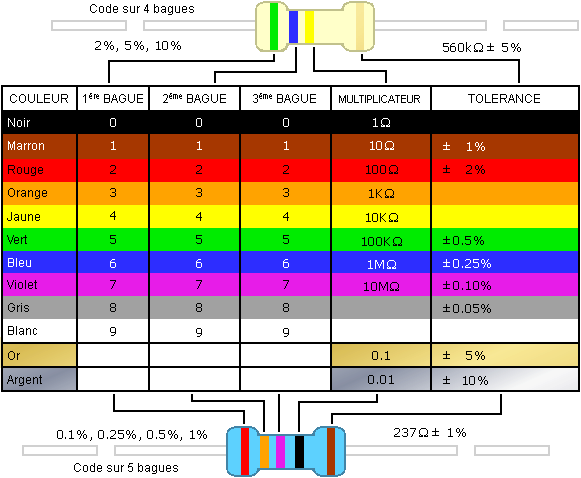
\includegraphics[scale=0.75]{Images/Code_couleur_resistance.png}
	\caption{Code des couleurs des résistances
		\label{Code_couleur_resistance}}
\end{figure}

La première bague est celle au ras du boitier, les autres bagues étant accolées à celle-ci.\\
Et voici une petite astuce mnémotechnique pour se rappeler de l'ordre des couleurs : \og{}Ne Manger Rien Ou Jeuner Voilà Bien Votre Grande Bêtise\fg{}.

\subsection{Séries normalisées}

Les valeurs des résistances sont standardisées et plusieurs séries de valeur existent :

\begin{itemize}
	\item E6 : 10, 15, 22, 33, 47, 68 ;
	\item E12 : 10, 12, 15, 18, 22, 27, 33, 39, 47, 56, 68, 82 ;
	\item E24 : 10, 11, 12, 13, 15, 16, 18, 20, 22, 24, 27, 30, 33, 36, 39, 43, 47, 51, 56, 62, 68, 75, 82, 91 ;
	\item E48 ...
\end{itemize}

\textit{Remarque :} pour un meilleur étalement, les séries sont telles que le rapport entre deux valeurs successives est identique. Par exemple, dans la série E6, ce rapport est égal à 1,47 environ (10 à la puissance 1/6).\\
Il est intéressant de se limiter à de petites séries, si possible E6, ce qui permet de faire des économies et être assuré d'avoir ces résistances de disponibles.

\subsection{La résistance de tirage}

% http://www.seattlerobotics.org/encoder/mar97/basics.html

La fonction de base d'une résistance de tirage est d'assurer que le circuit prenne une valeur logique par défaut en entrée, lorsque celle-ci n'est pas fixée par ailleurs. On parle de résistance pull-up (\textit{tirage vers le haut}), ainsi que de résistance pull-down (\textit{tirage vers le bas}), selon que l'entrée est fixée à l'état haut ou à l'état bas respectivement.

\begin{figure}[H]
	\centering
	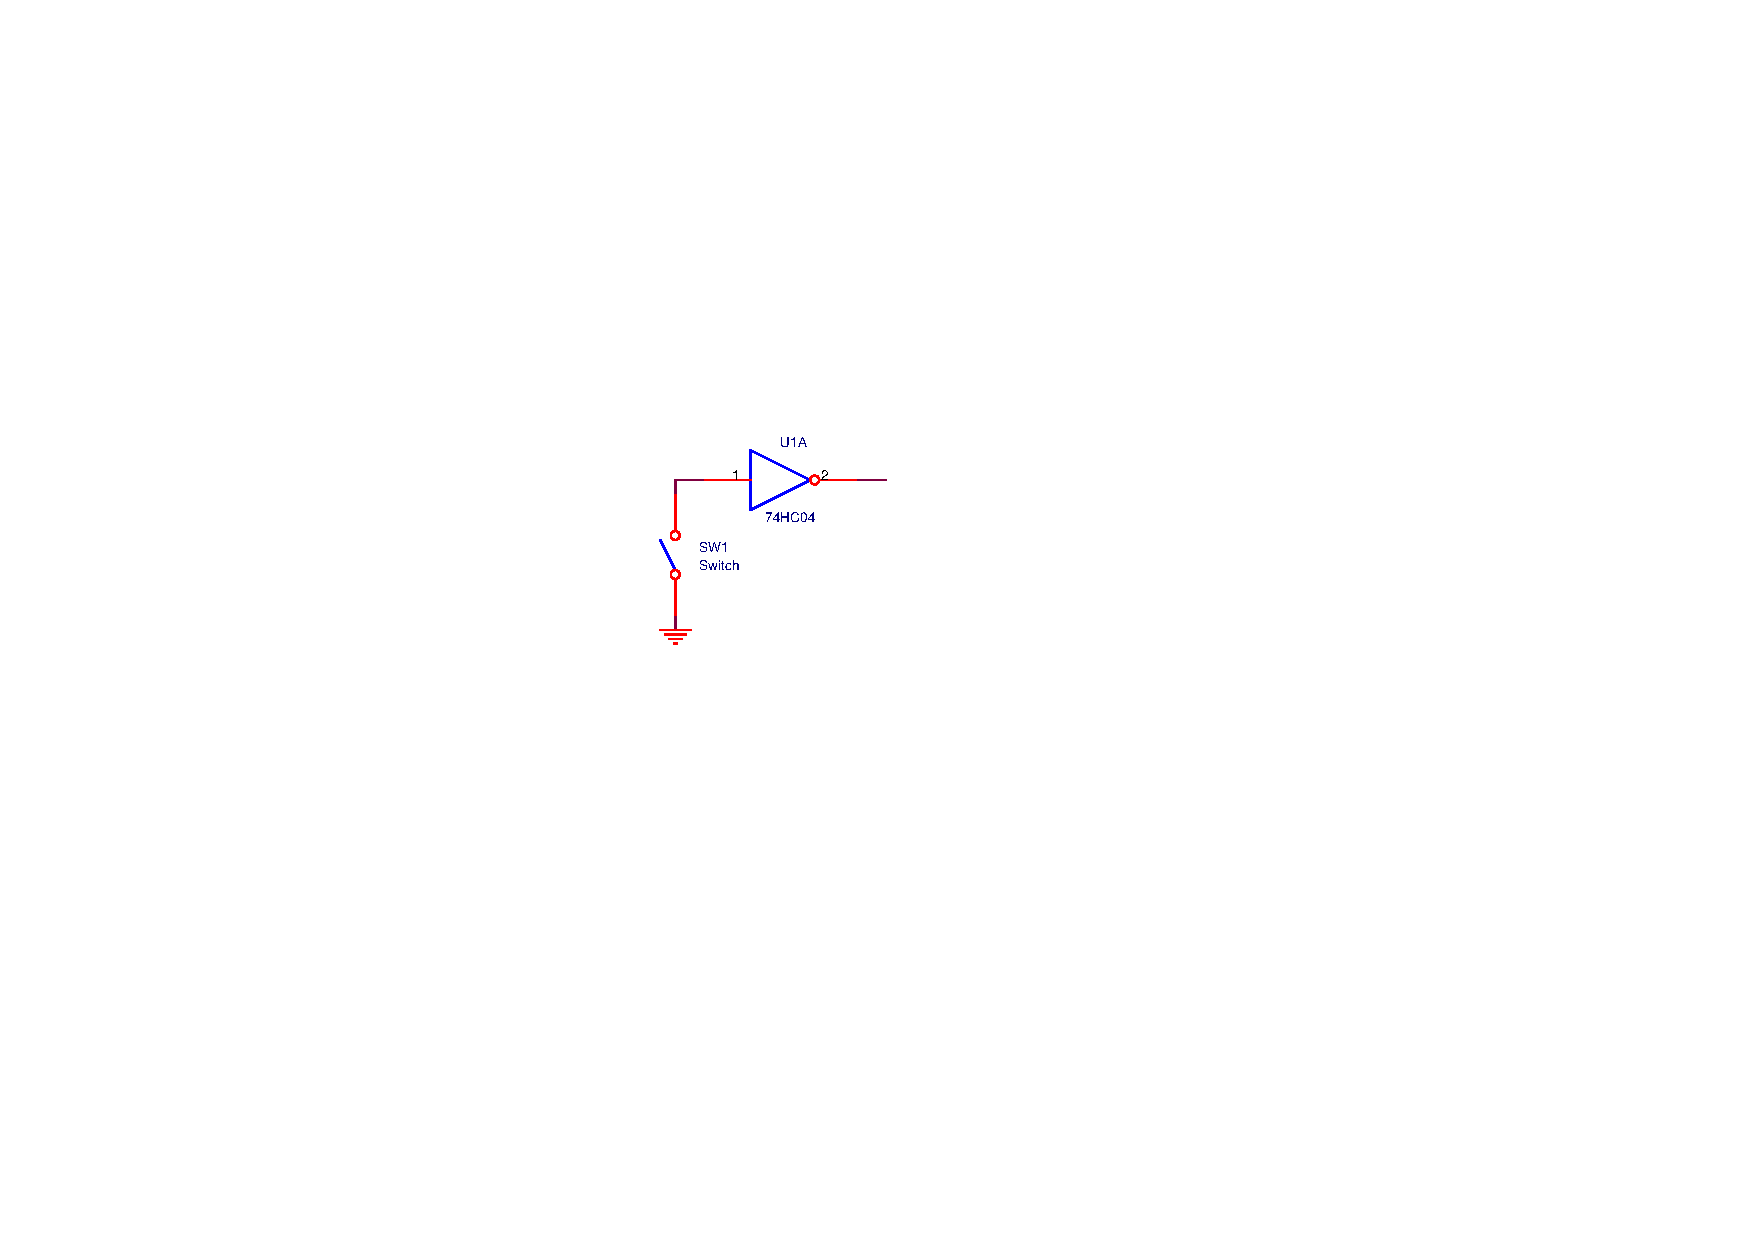
\includegraphics[scale=1.00]{Images/Switch_sans_pull-up}
	\caption{Switch sans pull-up
		\label{Switch_sans_pull-up}}
\end{figure}

Sur le schéma de la figure \ref{Switch_sans_pull-up}, la porte U1A a une entrée (pin 1) et une sortie (pin 2). La plupart des circuits logiques ont leurs entrées en état de haute impédance, ce qui signifie que si rien n'est connecté à la pin 1 du circuit logique précédent (ce qui est le cas lorsque l'interrupteur est ouvert), le potentiel à cette broche est flottant. Un potentiel flottant peut être considéré comme étant un 1 logique par la porte (par exemple, sachant que c'est généralement le cas), mais le moindre bruit électronique peut l'amener tantôt à l'état haut, tantôt à l'état bas. Ainsi, un simple bout de piste peut faire antenne et engendrer des perturbations suffisantes pour faire changer l'état du circuit logique.\\
Afin de fixer le potentiel même lorsque l'interrupteur est ouvert, il faut ajouter une résistance de tirage, comme illustré sur la figure \ref{Switch_avec_pull-up}.

\begin{figure}[H]
	\centering
	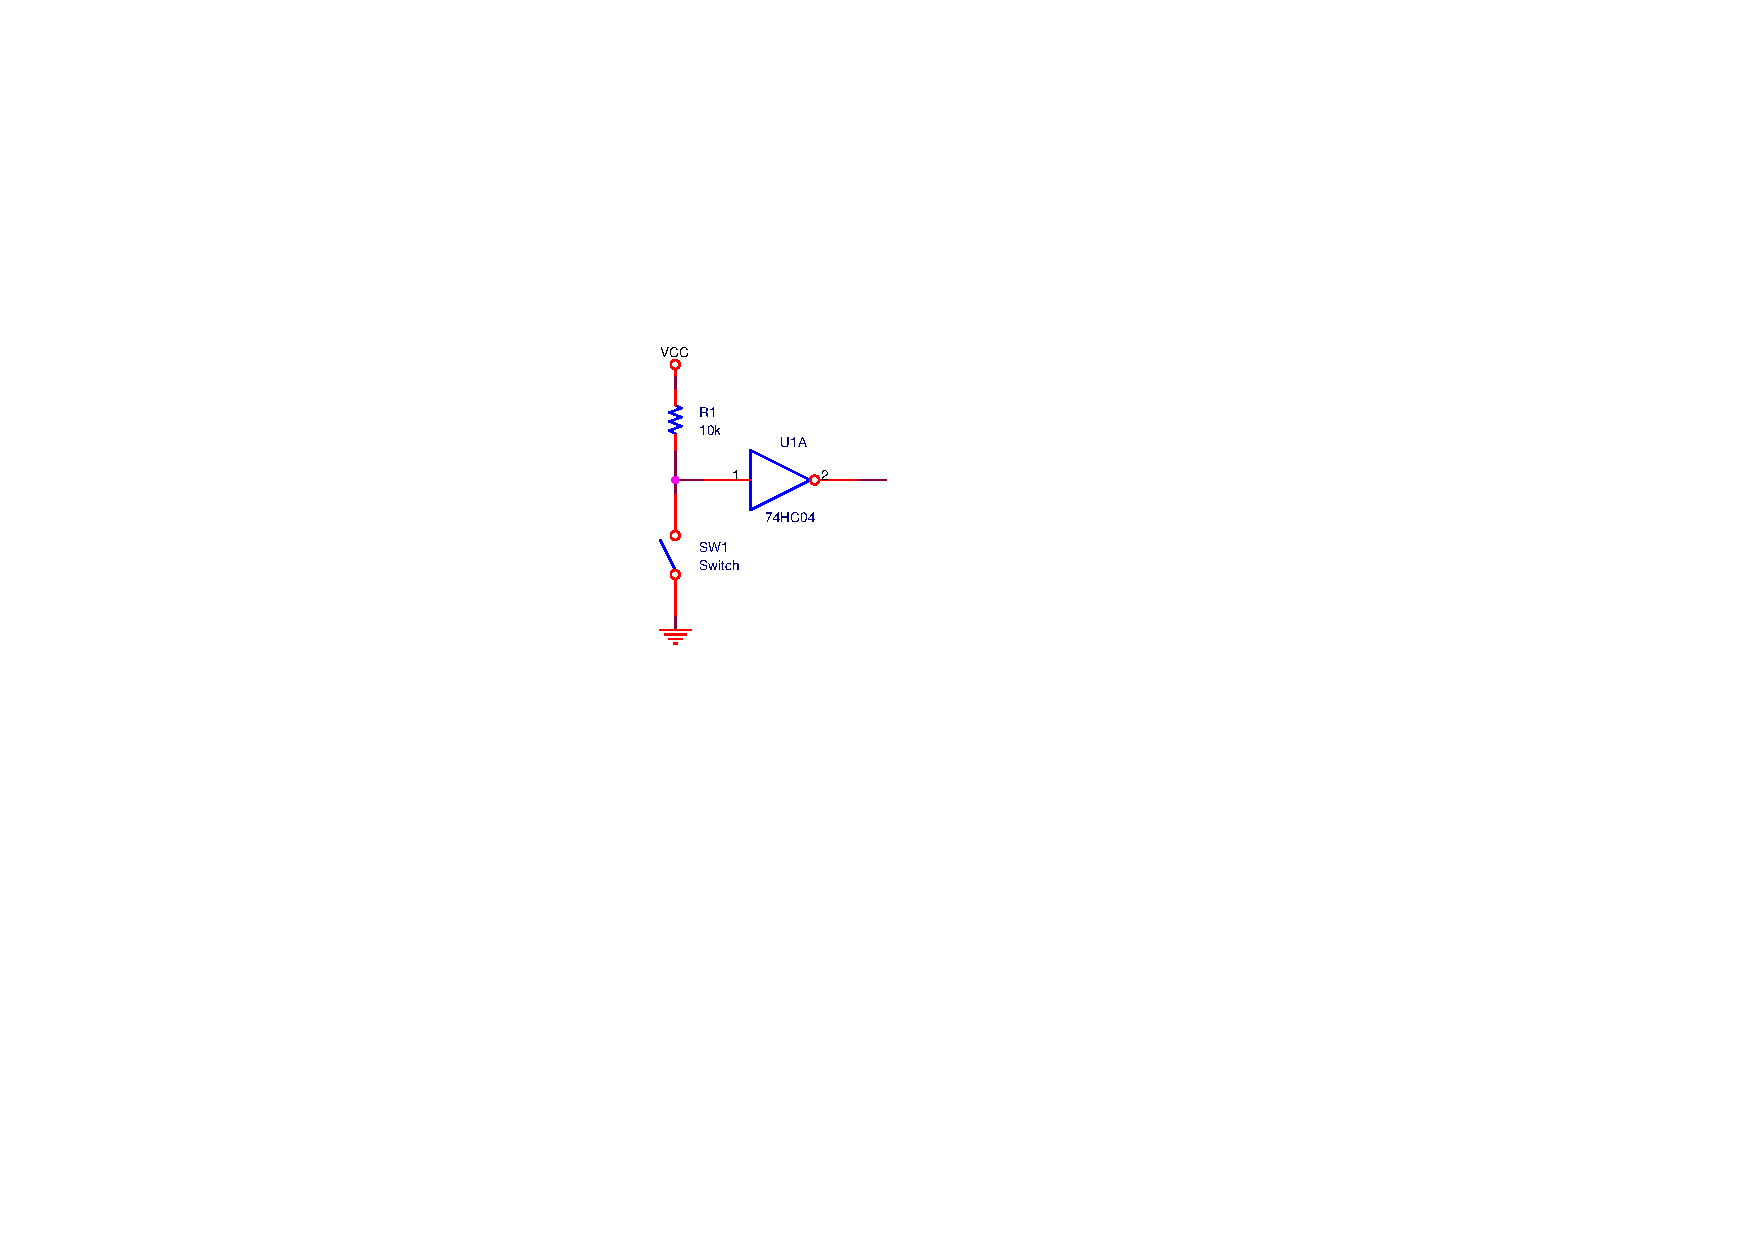
\includegraphics[scale=1.00]{Images/Switch_avec_pull-up}
	\caption{Switch avec pull-up
		\label{Switch_avec_pull-up}}
\end{figure}

Sans résistance on aurait un court-circuit franc lors de la fermeture de l'interrupteur, ce qui peut engendrer un courant très important de VCC à la masse susceptible de faire chauffer et bruler les pistes (qui font alors office de fusibles) ainsi que les composants. De plus, VCC serait ramené à un potentiel quasiment nul ce qui empêchera le circuit logique de fonctionner !\\
La résistance permet donc de limiter le courant lorsque l'interrupteur est fermé, tout en assurant la mise à 0 de la pin 1 du circuit logique sans perturbation du potentiel de VCC.\\
Une rapide loi d'Ohm permet de calculer le courant circulant alors dans la résistance :
\[I = \frac{VCC}{R1} = \frac{5 V}{10 k\Omega} = 0,5 mA\]
Lorsque l'interrupteur est ouvert, la pin 1 est mise à l'état haut au travers de la résistance de tirage.

\par
Il est clair que plus la résistance de tirage est grande, plus le courant la traversant sera faible et moins elle consommera :
\[P = \frac{VCC^{2}}{R1} = \frac{5^{2}}{10000} = 2,5 mW\]
Cependant, les circuits logiques ont généralement besoin d'un courant minimum en entrée pour fixer leur niveau logique (courant certes très faible et souvent approximé à 0), si bien qu'une résistance trop importante ne fonctionnera pas. Le courant minimum à fournir en entrée varie d'un circuit logique à l'autre et est en général indiqué dans sa datasheet, cependant des résistances de 10 k$\Omega$ à 47 k$\Omega$ peuvent être utilisées sans risque avec la grande majorité des circuits logiques (10 k$\Omega$ étant la valeur la plus courante).

\begin{figure}[H]
	\centering
	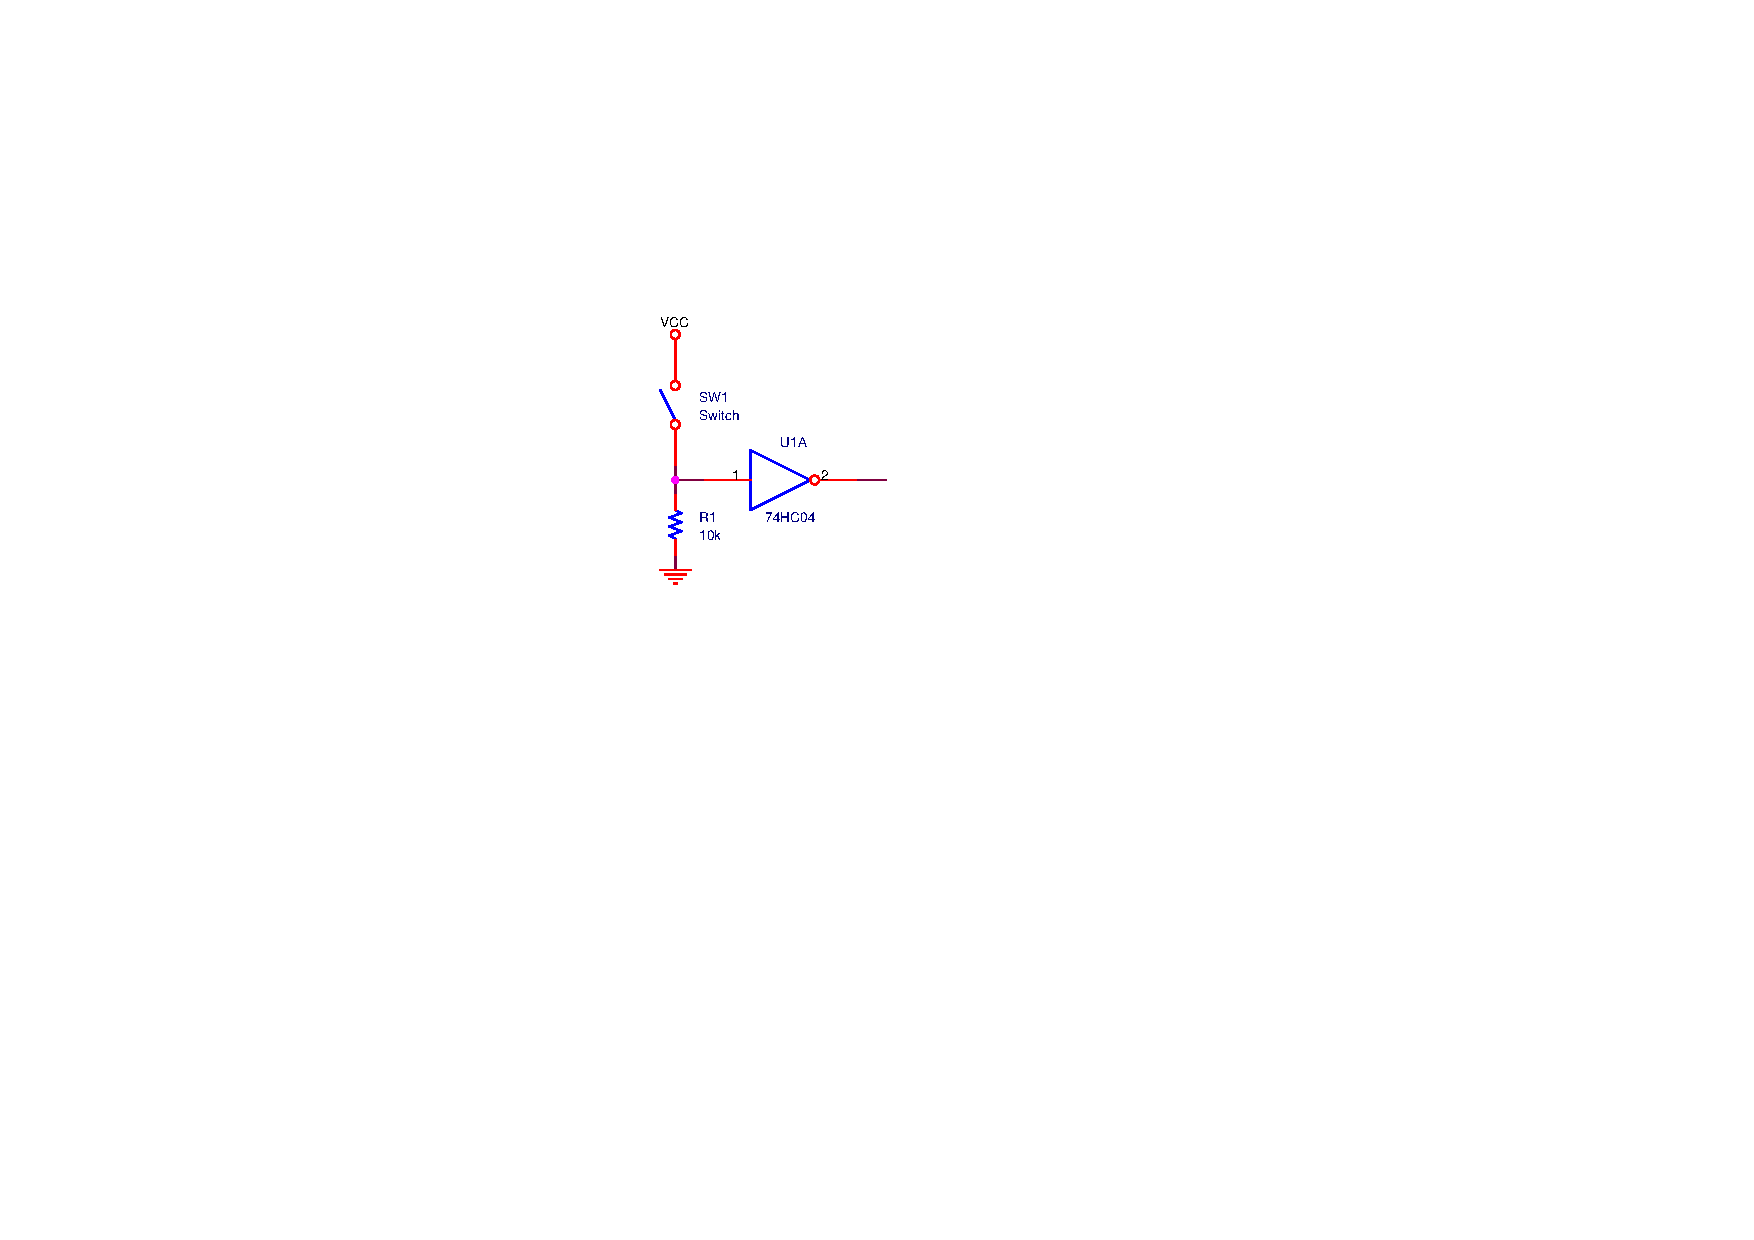
\includegraphics[scale=1.00]{Images/Switch_avec_pull-down}
	\caption{Switch avec pull-down
		\label{Switch_avec_pull-down}}
\end{figure}

La figure \ref{Switch_avec_pull-down} présente sur le même principe une résistance pull-down, qui permet d'imposer un niveau bas par défaut contrairement à la pull-up qui impose par défaut un niveau haut. Bien que moins courante, la résistance de pull-down est tout à fait valable, par exemple dans le cas où une pin non inverseuse d'un circuit logique doit être mise à 0 par défaut.

\subsection{La résistance de limitation de courant}

Dans cette section, nous allons voir un exemple simple d'utilisation d'une résistance de limitation de courant avec une broche de sortie d'un circuit logique et une \ac{LED}. Contrairement à une broche d'entrée, qui est en haute impédance, une broche de sortie a toujours au moins deux états possibles : état haut et état bas.

\subsubsection{Structure interne des sorties des circuits logiques}

Afin de comprendre pourquoi on utilise des résistances de limitation de courant, nous allons d'abord voir ce qui se passe lorsque l'on connecte une sortie d'un circuit logique sur une entrée d'un circuit logique. Pour cela, prenons l'exemple du 74HC04, qui n'est q'une simple porte inverseuse. On peut voir figure \ref{Structure_interne_74HC04} la structure interne, très simplifiée, mais tout à fait valide sur le principe, du circuit 74HC04. Quand un courant est appliqué sur la pin 1, le transistor devient passant et la pin 2 se retrouve au potentiel 0. Le transistor joue ici le rôle d'un interrupteur commandé.

\begin{figure}[H]
	\centering
	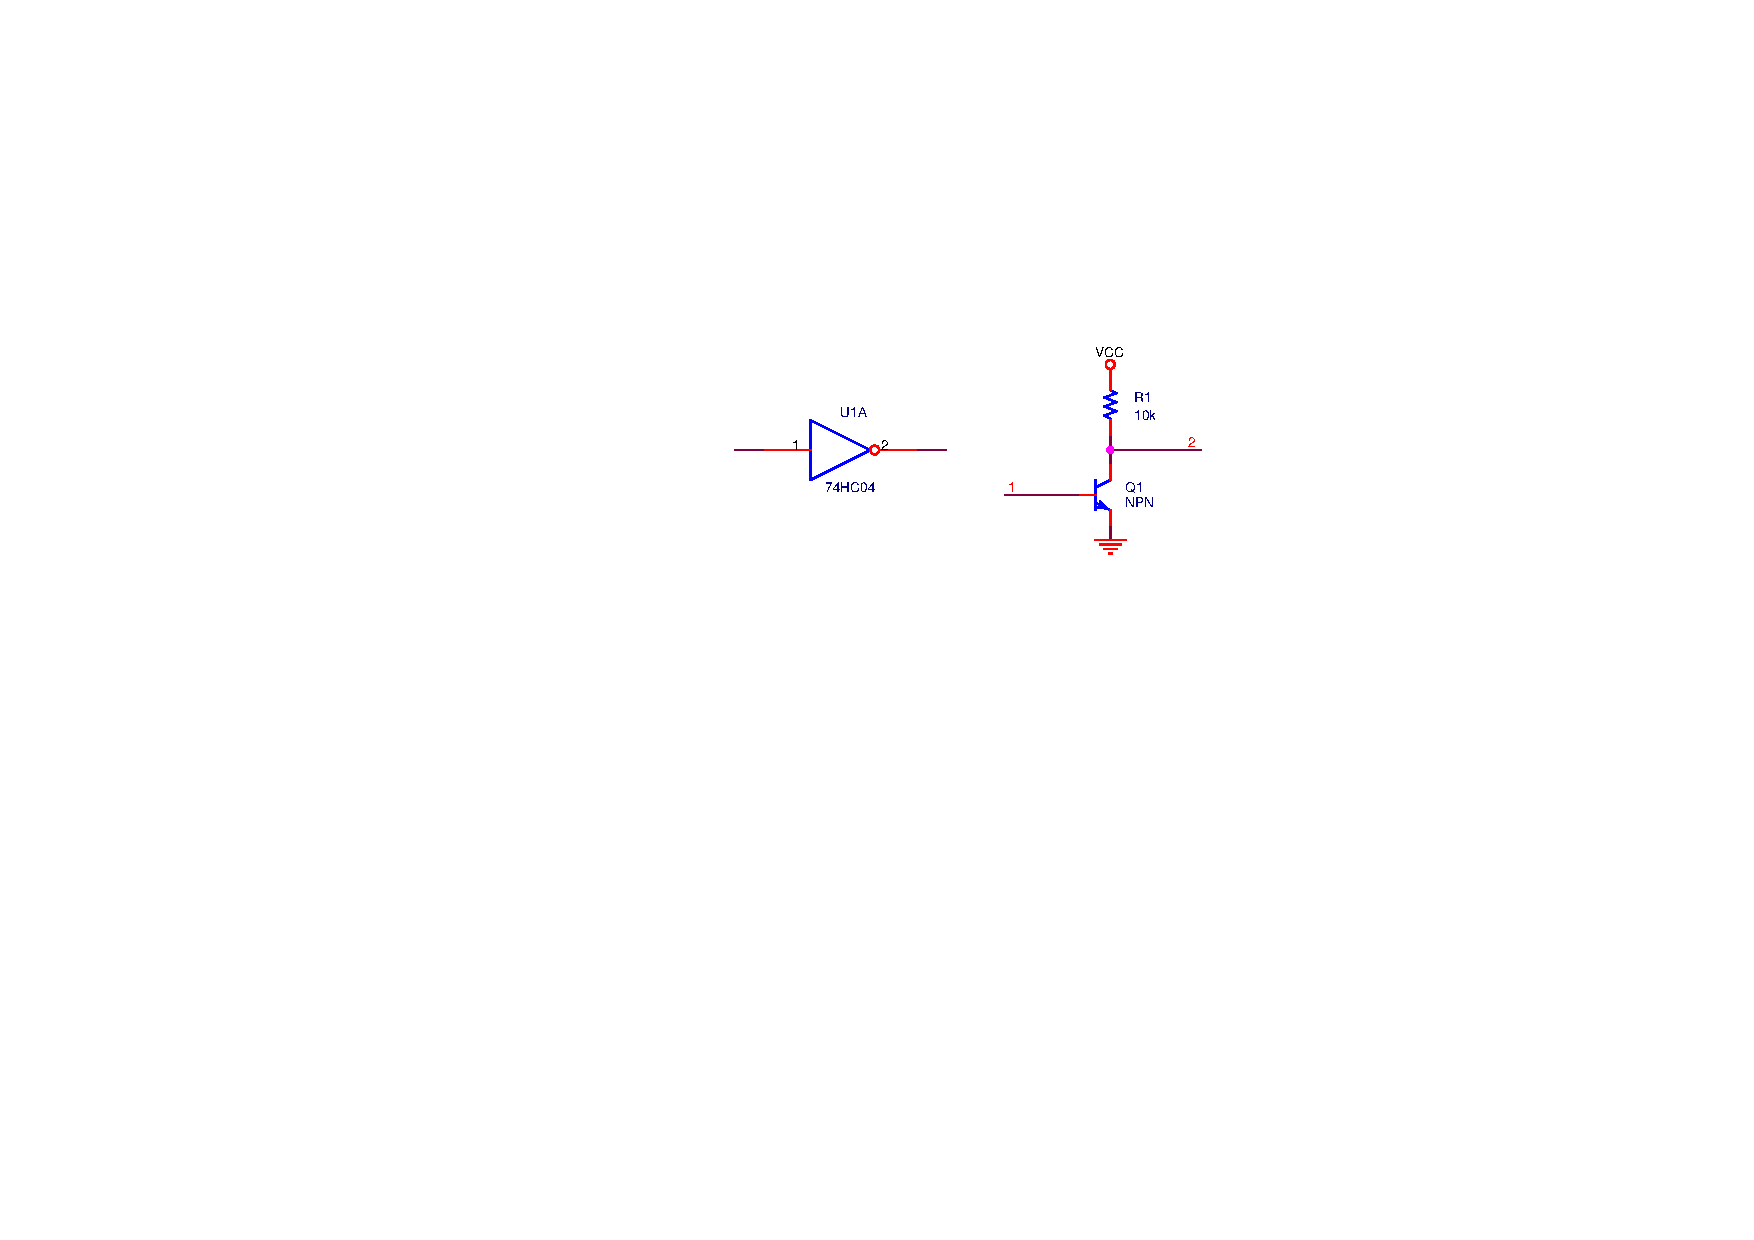
\includegraphics[scale=1.00]{Images/Structure_interne_74HC04}
	\caption{Structure interne du 74HC04
		\label{Structure_interne_74HC04}}
\end{figure}

Cette structure est intéressante, car elle représente également la structure interne de base des sorties (2 états) de n'importe quel circuit logique, qui sont en fait des interrupteurs commandés par des transistors. On constate donc que les broches de sortie utilisent une résistance pull-up.

\begin{figure}[H]
	\centering
	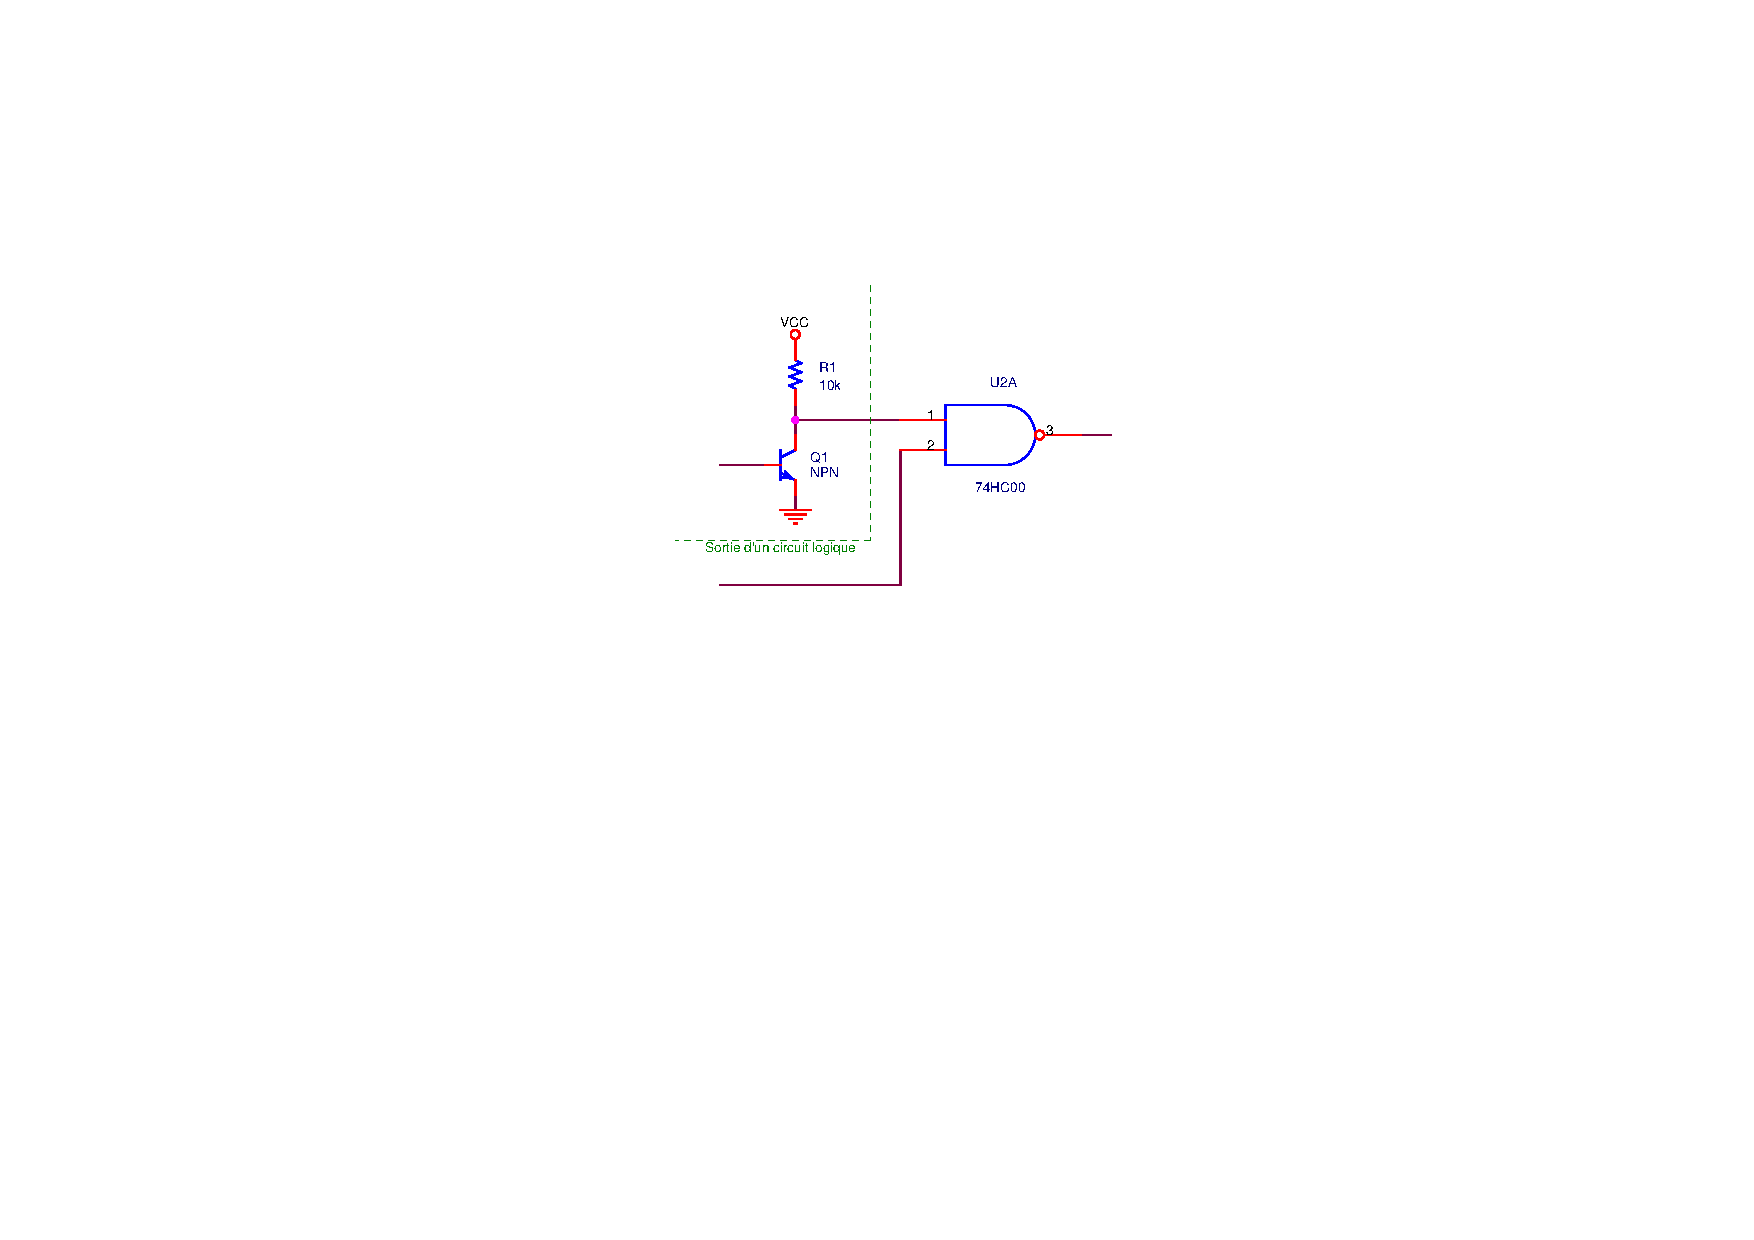
\includegraphics[scale=1.00]{Images/Montage_sortie_circuit_logique}
	\caption{Structure interne d'une sortie d'un circuit logique
		\label{Montage_sortie_circuit_logique}}
\end{figure}

Si l'on branche une sortie sur une entrée d'un deuxième circuit logique, comme illustré figure \ref{Montage_sortie_circuit_logique}, lorsque Q1 est bloqué, R1 assure le niveau logique haut sur l'entrée de U2A, tandis que lorsque Q1 est passant, l'entrée d'U2A est mise à 0. La résistance pull-up R1 (qui est rappelons-le une résistance interne) assure le passage d'un courant suffisant pour imposer les bons niveaux logiques au circuit U2A, sans avoir à ajouter de résistance de pull-up supplémentaire. Ainsi, pour la plupart des circuits logiques, on peut directement connecter une sortie sur une entrée d'un autre circuit.

\subsubsection{Montage d'une LED sur la sortie d'un circuit logique}

Considérons désormais le cas où la sortie d'un circuit logique n'est pas une entrée d'un autre circuit logique. Par exemple, on aimerait commander une \ac{LED} avec cette sortie. Il est alors nécessaire de prendre certaines précautions et de considérer le cas où la sortie est mise à l'état bas, ce qui équivaut à une connexion directe avec la masse. Dans ce cas, il est important de contrôler le courant qui va circuler dans la sortie du circuit logique. La plupart des circuit logiques peuvent supporter sur leurs sorties un courant allant jusqu'à 20 mA (par broche).

Il faut savoir qu'une \ac{LED} par exemple, a une résistance interne très faible. Lorsqu'elle est passante, elle ne va donc pas limiter le courant et risque de fondre si celui-ci est trop important. De même, si l'on connecte directement cette \ac{LED} entre VCC et la sortie du circuit logique, la mise à l'état bas de celle-ci équivaudrait pratiquement à court-circuiter VCC avec la masse, ce qui pourrait provoquer la destruction du circuit logique en plus de la \ac{LED}. Avant de connecter la \ac{LED} sur une sortie d'un circuit logique, il faut donc connaitre le courant maximum admissible par celle-ci, sachant qu'il ne faut de toute manière pas dépasser les 20 mA que peut supporter la sortie.

\begin{figure}[H]
	\centering
	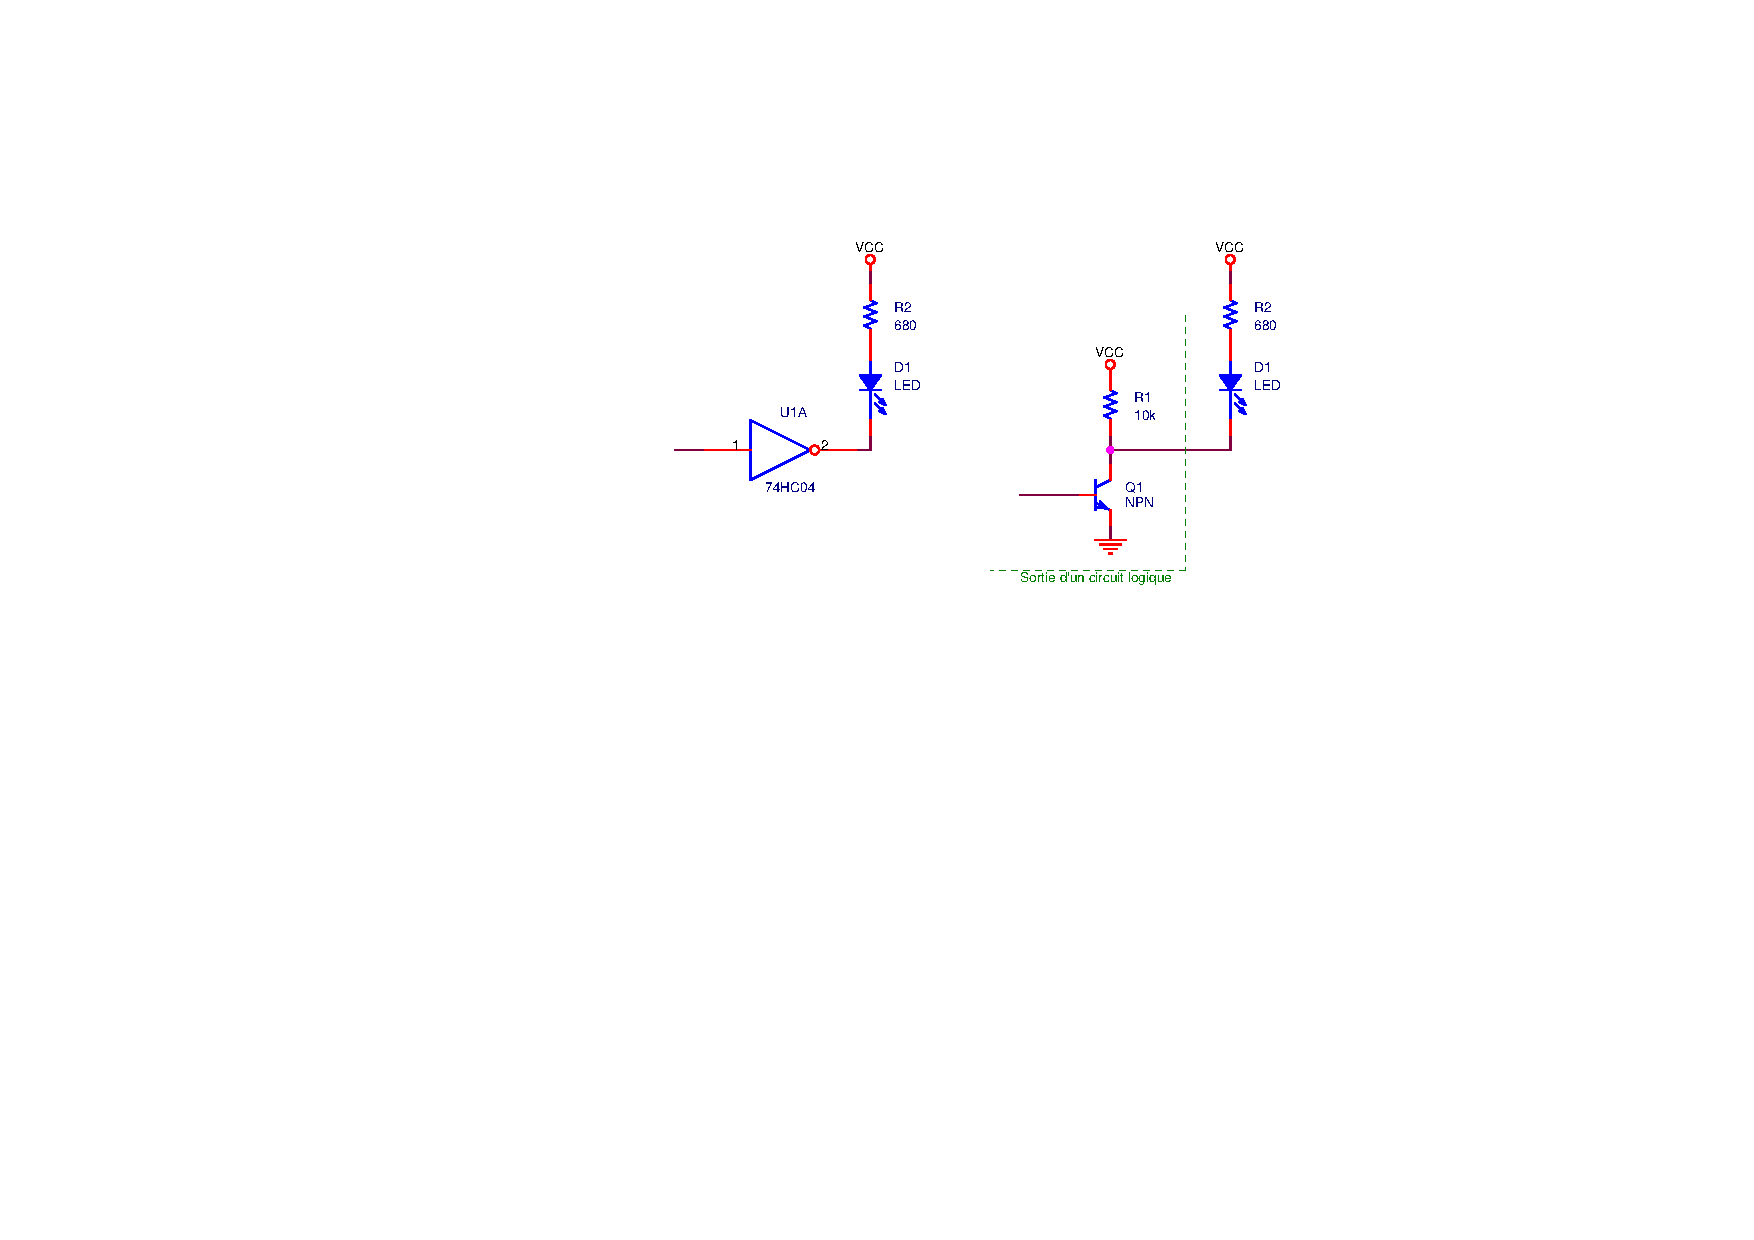
\includegraphics[scale=1.00]{Images/Montage_LED_resistance_limitation}
	\caption{Montage d'une \ac{LED} avec résistance de limitation
		\label{Montage_LED_resistance_limitation}}
\end{figure}

Le courant maximal est fixé avec une résistance de limitation de courant. En considérant que la plupart des \acp{LED} supportent au moins 15 mA, si VCC = 5V, la loi d'Ohm nous donne la valeur minimum de la résistance à utiliser :
\[R = \frac{VCC}{I} = \frac{5 V}{15 mA} = 333 \Omega\]

On peut se donner une marge et limiter la puissance consommée en prenant une valeur de résistance plus importante (mais pas trop quand même pour ne pas trop diminuer la luminosité de la \ac{LED}). Une valeur couramment utilisée pour une \ac{LED} de base est 680 $\Omega$.

Le montage avec résistance de limitation est donné figure \ref{Montage_LED_resistance_limitation} : quand la broche de sortie est à l'état haut, la \ac{LED} est bloquée (différence de potentiel à ses bornes nulle) et lorsque la broche de sortie est à l'état bas, la \ac{LED} est passante et tout se passe comme si la pin 2 du circuit logique était directement connecté à la masse.

\subsection{Les résistances de puissance}

La figure \ref{Resistances_puissance} montre quelques résistances de puissance, rangées dans l'ordre croissant de puissance, de gauche à droite. Parce qu'il n'est pas toujours évident de deviner qu'il s'agit de résistances...

\begin{figure}[H]
	\centering
	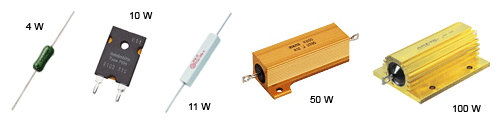
\includegraphics[scale=0.75]{Images/Resistances_puissance.png}
	\caption{Quelques résistances de puissance
		\label{Resistances_puissance}}
\end{figure}

\subsection{Les réseaux de résistances}

Les réseaux de résistances sont très pratiques pour des résistances de tirage, entre un switch et un circuit logique par exemple, ou lorsqu'on a besoin de plusieurs résistances identiques et que l'on veut gagner de la place.

Il y a deux types principaux de réseaux de résistances : plusieurs résistances indépendantes (schéma de gauche figure \ref{Reseaux_resistances_schema}), ou des résistances avec un commun (schéma de droite).

\begin{figure}[H]
	\centering
	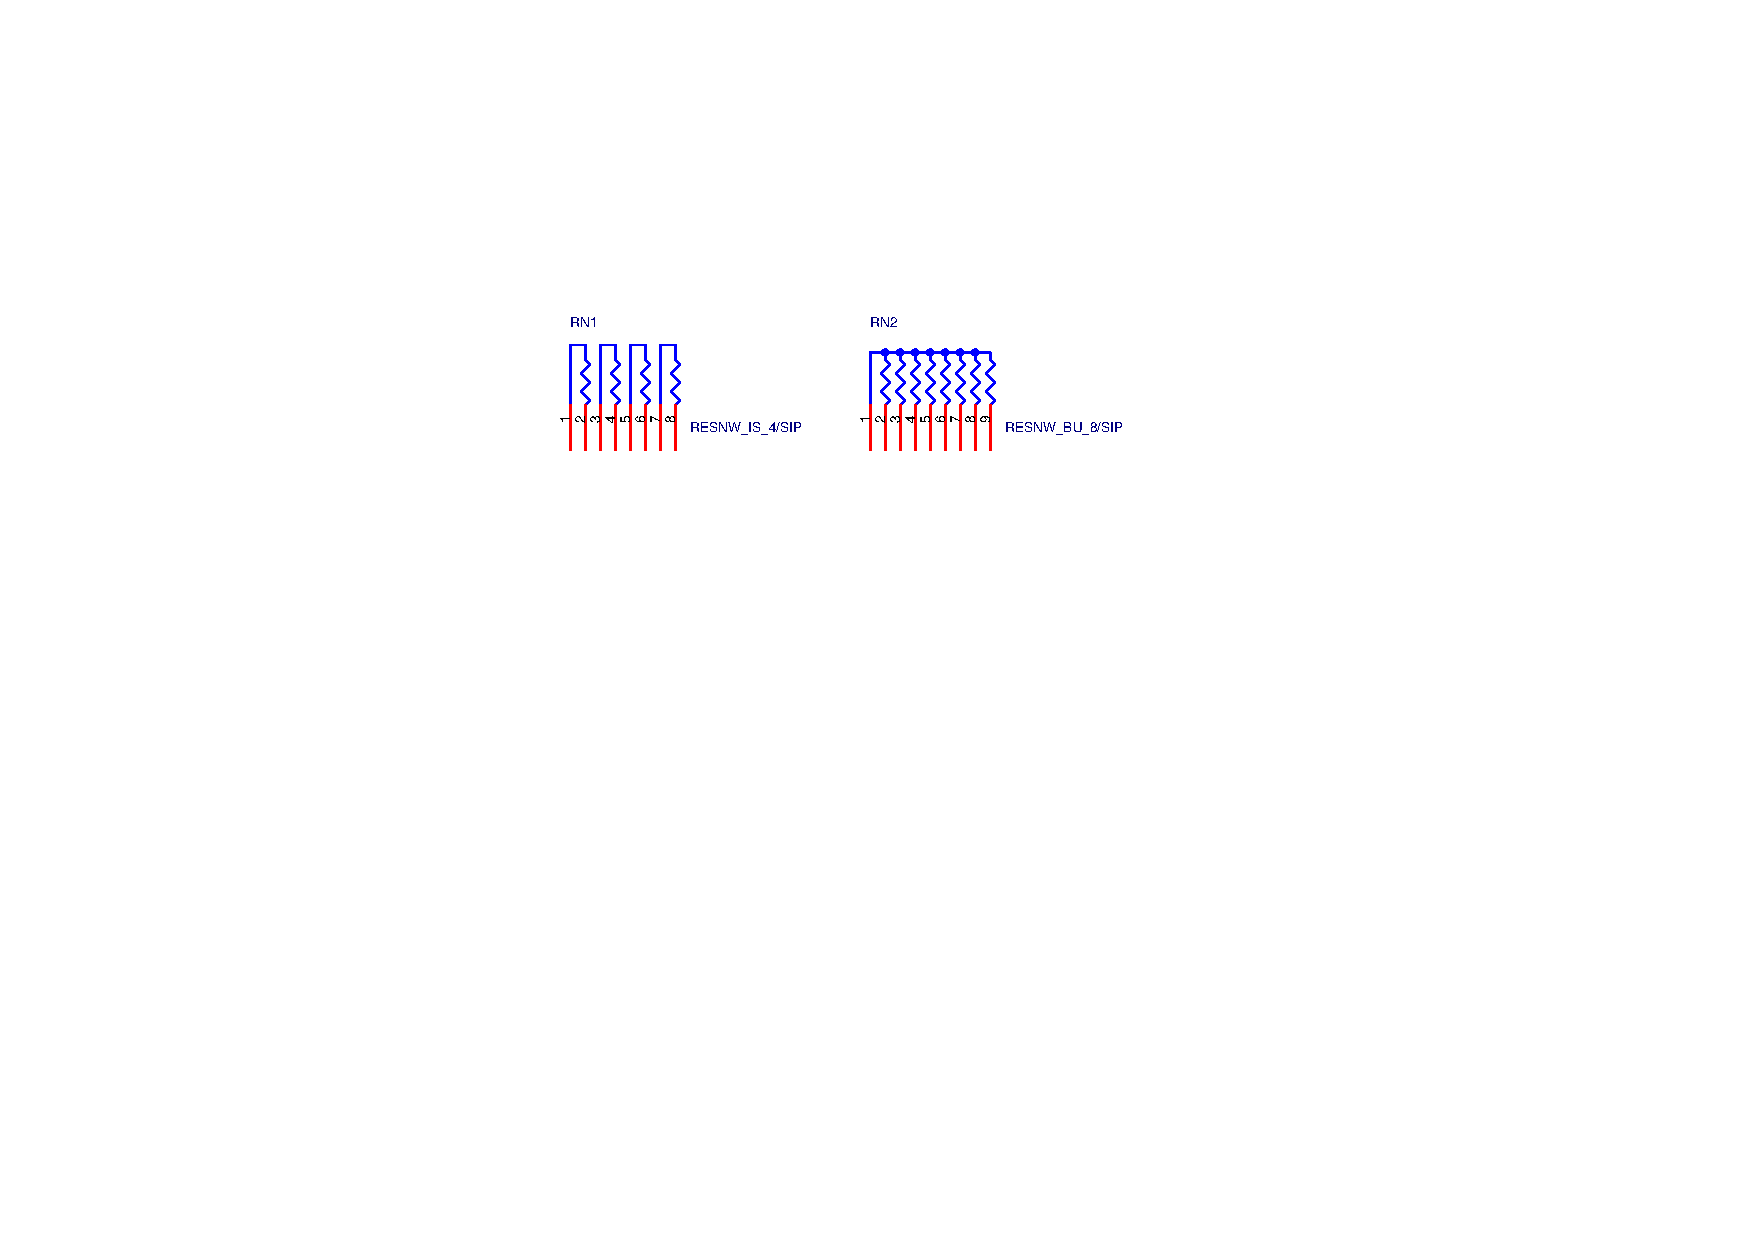
\includegraphics[scale=1.00]{Images/Reseaux_resistances_schema}
	\caption{Schéma de réseaux de résistances
		\label{Reseaux_resistances_schema}}
\end{figure}

Le point sur le réseau permet de repérer la première broche (le commun, s'il s'agit du deuxième type de réseau), figure \ref{Reseaux_resistances}.

\begin{figure}[H]
	\centering
	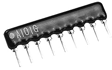
\includegraphics[scale=0.75]{Images/Reseaux_resistances.png}
	\caption{Un réseau de résistances
		\label{Reseaux_resistances}}
\end{figure}

\section{Les condensateurs}

% http://www.planete-sciences.org/robot/wikibot/index.php/Condensateur
% http://licencer.free.fr/condos.html
% http://www.chez.com/xizard/Cours/Condensateur_index.htm
% http://perso.orange.fr/f5zv/RADIO/RM/RM24/RM24G/RM24G.HTM
% http://www.interq.or.jp/japan/se-inoue/e_capa.htm
% http://www.uoguelph.ca/~antoon/gadgets/caps/caps.html
% http://my.execpc.com/~endlr/markings.html

\subsection{Principales caractéristiques}

\begin{itemize}
	\item \textbf{La capacité}, exprimée en farads (F) ;
	\item \textbf{La tension nominale} en courant continu : exprimée en volts continus, il s'agit de la tension maximale que peut supporter en permanence le condensateur à ses bornes. Une tension supérieure peut provoquer l'explosion du composant ;
	\item \textbf{La tolérance}, qui indique les écarts de valeur maximum que peut avoir la capacité du condensateur, exprimée en \% par rapport à sa valeur idéale ;
	\item \textbf{Déviation en température} : la capacité des condensateurs varie avec la température. Cette variation peut être positive (augmentation de la capacité), ou négative (diminution). Elle s'exprime en ppm/°C (pour rappel, 1 ppm = une partie par million = 0,000\,1\%) ;
	\item \textbf{Courant de fuite} : le condensateur, même isolé, se décharge au cours du temps, via un courant de fuite circulant entre ses deux broches, qui peut être de l'ordre du mA ;
	\item \textbf{Résistance série} : les condensateurs n'étant pas parfaits, on associe en série à la capacité une résistance, de très faible valeur (généralement très inférieur à l'ohm).
\end{itemize}

\subsection{Les types de condensateurs}

\subsubsection{Céramiques}

\begin{figure}[H]
	\centering
	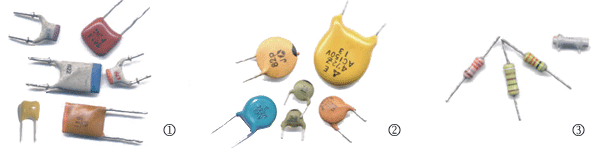
\includegraphics[scale=0.75]{Images/Condensateurs_ceramique.png}
	\caption{Condensateurs céramique
		\label{Condensateurs_ceramique}}
\end{figure}

\begin{enumerate}
	\item A plaquette ;
	\item A disque ;
	\item Tubulaire (pas courant).
\end{enumerate}

\begin{table}[H]
	\centering
		\begin{tabular}{|l|l|l|l|l|}\hline
				Classe & Capacité & Série & Tolérance & Tension supportée\\\hline\hline
				I & 1 pF à 100 nF & E12 & $\pm$5 à $\pm$10\% & 50 V à 100 V\\\hline
				II & 100 pF à 4,7 $\mu$F & E6 & $\pm$10\% & 50 V à 100 V\\\hline
				III & 1 nF à 4,7 $\mu$F & E3 & $\pm$20\% ou plus & 50 V à 100 V\\\hline
		\end{tabular}
		\caption{Caractéristiques typiques des condensateurs céramique
			\label{Caracteristiques_des_condensateurs_ceramique}}
\end{table}

Il existe en tout 4 classes de condensateurs céramique, dans la classification de l'\ac{EIA}. Plus la classe est petite, meilleur sont les caractéristiques du condensateur.

\paragraph{Emploi}

L'utilisation des condensateurs céramique est très large, voici plutôt les cas où l'on utilise de préférence d'autres types de condensateurs :

\begin{itemize}
	\item dans les oscillateurs où une grande stabilité de capacité est requise, on préfère les condensateurs au mica, au polystyrène ou au polycarbonate ;
	\item dans les circuits de filtrage et de découplage où une très grande capacité est requise, on utilise les condensateurs électrolytiques (aluminium et tantale) ;
	\item dans les circuits à basse fréquence car leur capacité est généralement trop faible.
\end{itemize}

\subsubsection{A film plastique (MK)}

\begin{figure}[H]
	\centering
	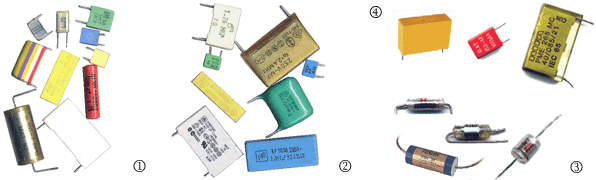
\includegraphics[scale=0.75]{Images/Condensateurs_plastique.png}
	\caption{Condensateurs plastique
		\label{Condensateurs_plastique}}
\end{figure}

\begin{enumerate}
	\item (M)KT : polyester (polyéthylène ou mylar) ;
	\item (M)KP : polypropylène ;
	\item (M)KS : polystyrène (styroflex) ;
	\item (M)KC : polycarbonate.
\end{enumerate}

La présence d'un \og{}M\fg{} signifie que le condensateur est à film métallisé.

\begin{table}[H]
	\centering
		\begin{tabular}{|l|l|l|l|l|}\hline
				Type & Capacité & Série & Tolérance & Tension supportée\\\hline\hline
				Polyester & 1 nF à 15 $\mu$F & E12 & 10\% & 50 V à 1\,500 V\\\hline
				Polypropylène & 100 pF à 10 $\mu$F & E12 & 10\% & 63 V à 2\,000 V\\\hline
				Polystyrène & 10 pF à 47 nF & E12 & 10\% & 30 V à 630 V\\\hline
				Polycarbonate & 100 pF à 15 $\mu$F & E12 & 10\% & 63 V à 1\,000 V\\\hline
		\end{tabular}
		\caption{Caractéristiques typiques des condensateurs plastique
			\label{Caracteristiques_des_condensateurs_plastique}}
\end{table}

\paragraph{Emploi}

\begin{itemize}
	\item Polyester (caractéristiques plutôt médiocres) : circuits BF, découplage, filtrage et applications où les rapports performances / prix et capacité / encombrement doivent être grands ;
	\item Polypropylène (ses propriétés se dégradent en HF) : circuits accordés, alimentations, BF ;
	\item Polystyrène (bonnes caractéristiques, peu de pertes) : circuits accordés HF, alimentations, BF, timer, filtres ;
	\item Polycarbonate (très stable) : circuits BF, découplage, filtrage.
\end{itemize}

Pris ensembles, les condensateurs à film plastique satisfont à la plupart des usages de l'électronique courant.

\subsubsection{Électrolytiques}

\paragraph{Électrolytiques aluminium (chimique)}

Ce type de condensateur est polarisé dans la plupart des cas.

\begin{figure}[H]
	\centering
	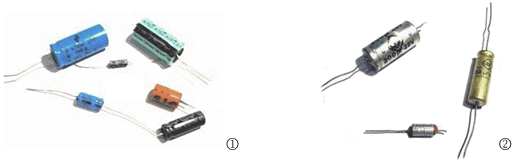
\includegraphics[scale=0.75]{Images/Condensateurs_chimique.png}
	\caption{Condensateurs chimique
		\label{Condensateurs_chimique}}
\end{figure}

\begin{enumerate}
	\item Polarisé ;
	\item Non polarisé.
\end{enumerate}

\begin{table}[H]
	\centering
		\begin{tabular}{|l|l|l|l|l|}\hline
				Capacité & Série & Tolérance & Tension supportée\\\hline
				0,1 $\mu$F à 68 mF & E6 & 20\% & jusqu'à 450 V\\\hline
		\end{tabular}
		\caption{Caractéristiques typiques des condensateurs chimique
			\label{Caracteristiques_des_condensateurs_chimique}}
\end{table}

\subparagraph{Emploi}

Partout où une forte valeur est exigée, filtrage, découplage, lissage, ligne de retard...

\subparagraph{Problèmes connus}

Ce type de condensateur vieilli (la capacité diminue au fil du temps) et il faut se méfier particulièrement des récupérations, surtout si le montage à effectuer requiert de la précision, d'autant plus qu'un condensateur récent de ce type sera plus petit qu'un vieux aux caractéristiques identiques, comme le montre la figure \ref{Condensateur_chimique_age}.

\begin{figure}[H]
	\centering
	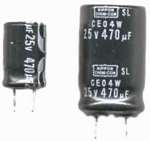
\includegraphics[scale=0.75]{Images/Condensateur_chimique_age.png}
	\caption{Comparaison entre un ancien et un condensateur chimique récent, aux caractéristiques identiques (25 V, 470 $\mu$F)
		\label{Condensateur_chimique_age}}
\end{figure}

Un autre problème qui peut survenir avec ce type de condensateur, est son gonflement, dû à une fabrication défectueuse. Il s'en suit une perte significative de la capacité, qui a tendance à provoquer des instabilité par exemple sur des cartes de PC, où l'on rencontre parfois ce problème. Un condensateur ayant \og{}gonflé\fg{} ne peut plus être utilisé et doit être remplacé (voir figure \ref{Condensateurs_gonfles}).

\begin{figure}[H]
	\centering
	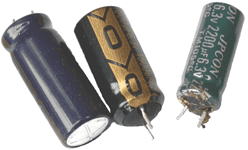
\includegraphics[scale=0.75]{Images/Condensateurs_gonfles.png}
	\caption{Condensateurs électrolytiques aluminium ayant gonflés (le 1\ier{} par dessus, le 2\ieme{} par dessous et du liquide électrolytique s'est échappé du 3\ieme{})
		\label{Condensateurs_gonfles}}
\end{figure}

\paragraph{Électrolytiques tantale}

Ces condensateurs sont également polarisés. La plus est généralement indiqué par un signe \og{}+\fg{} du coté de la broche correspondante.

\begin{figure}[H]
	\centering
	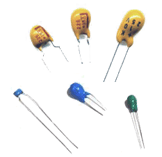
\includegraphics[scale=0.75]{Images/Condensateurs_tantale.png}
	\caption{Condensateurs tantale
		\label{Condensateurs_tantale}}
\end{figure}

\begin{table}[H]
	\centering
		\begin{tabular}{|l|l|l|l|l|}\hline
				Capacité & Série & Tolérance & Tension supportée\\\hline
				0,1 $\mu$F à 150 $\mu$F & E6 & 20\% & 6,3 V à 35 V\\\hline
		\end{tabular}
		\caption{Caractéristiques typiques des condensateurs tantale
			\label{Caracteristiques_des_condensateurs_tantale}}
\end{table}

\subparagraph{Emploi}

Temporisateurs de longue durée. Inconvénient : leur prix assez élevé.

\subsubsection{Au mica}

\begin{table}[H]
	\centering
		\begin{tabular}{|l|l|l|l|}\hline
				Capacité & Tolérance & Tension supportée\\\hline
				1 pF à 100 nF & 1 à 20\% & 300 V à plus de 2\,500 V\\\hline
		\end{tabular}
		\caption{Caractéristiques typiques des condensateurs au mica
			\label{Caracteristiques_des_condensateurs_au_mica}}
\end{table}

Les condensateurs au mica sont réservés à des applications nécessitant une grande stabilité, peu de pertes ou des tensions élevées, en raison de leur cout élevé.

\subsubsection{Au papier}

\begin{table}[H]
	\centering
		\begin{tabular}{|l|l|l|l|}\hline
				Capacité & Tolérance & Tension supportée\\\hline
				500 pF à 0,5 $\mu$F & 20\% & 125 V à 1\,000 V\\\hline
		\end{tabular}
		\caption{Caractéristiques typiques des condensateurs au papier
			\label{Caracteristiques_des_condensateurs_au_papier}}
\end{table}

Les condensateurs au papier ne s'utilisent plus que rarement, mais on le rencontre encore notamment dans les applications à haute tension où un condensateur non polarisé est nécessaire.

\subsection{Marquage des condensateurs}

Lorsque la taille le permet, la valeur des capacités est généralement clairement indiquée, comme sur les condensateurs électrolytiques par exemple. Sinon, il existe une large variété de codes, utilisant des caractères alphanumériques ou des couleurs, dont voici les principaux :

\subsubsection{Indication de la capacité}

\paragraph{Valeur sur 2 chiffres}

Il s'agit directement de la valeur du condensateur, en pico-farads (pF).

\paragraph{Valeur sur 3 chiffres}

Les 2 premiers chiffres indiquent une valeur en pico-farads (pF), tandis que le troisième est le multiplicateur (qui correspond dans la plupart des cas, mais pas toujours, au nombre de 0 à ajouter pour obtenir la valeur du condensateur, voir tableau \ref{Chiffre_multiplicateur}).

\begin{table}[H]
	\centering
		\begin{tabular}{|l|l|}\hline
				Chiffre & Multiplicateur\\\hline\hline
				0 & $\times$1\\\hline
				1 & $\times$10\\\hline
				2 & $\times$100\\\hline
				3 & $\times$1\,000\\\hline
				4 & $\times$10\,000\\\hline
				5 & $\times$100\,000\\\hline
				6 (non utilisé) & \\\hline
				7 (non utilisé) & \\\hline
				8 & $\times$0,01\\\hline
				9 & $\times$0,1\\\hline
		\end{tabular}
	\caption{Chiffre multiplicateur
		\label{Chiffre_multiplicateur}}
\end{table}

Il y a ambiguïté lorsque le 3\ieme{} chiffre est 0. Par exemple, \og{}560\fg{} pourrait signifier 560 pF, ou 56$\times$1 = 56 pF. En l'absence d'autre indication, il s'agit généralement de la première valeur qui est la bonne, le 3\ieme{} chiffre étant alors le dernier chiffre significatif, mais ce n'est pas certain.

\paragraph{Autres indications de la valeur}

Une lettre correspondant à un certain multiple du pico-farad (pF) est à la place de la virgule décimale (marquage européen).

\begin{table}[H]
	\centering
		\begin{tabular}{|l|l|}\hline
				Lettre & Multiplicateur\\\hline\hline
				p (pico) ou R (virgule décimale) & $\times$1\\\hline
				n (nano) & $\times$1\,000\\\hline
				$\mu$ ou u (micro) & $\times$1\,000\,000\\\hline
				m (milli) & $\times$1\,000\,000\,000\\\hline
		\end{tabular}
	\caption{Symbole multiplicateur
		\label{Symbole_multiplicateur}}
\end{table}

Par exemple, \og{}4n7\fg{} signifie 4,7 nF, ou encore, \og{}R47\fg{} signifie 0,47 pF.

\subsubsection{Indication de la tolérance}

Lorsque celle-ci n'est pas indiquée, la tolérance est généralement de $\pm$20\%.

\paragraph{Code tolérance}

Une lettre supplémentaire, juste après la valeur, indique en plus la tolérance, voir tableau \ref{Lettre_de_tolerance}.

\begin{table}[H]
	\centering
		\begin{tabular}{|l|l|}\hline
				Lettre & Tolérance\\\hline\hline
				A	& $\pm$0,05 pF\\\hline
				B	& $\pm$0,1 pF\\\hline
				C	& $\pm$0,25 pF\\\hline
				D	& $\pm$0,5 pF\\\hline
				E	& $\pm$0,5\%\\\hline
				F	& $\pm$1\%\\\hline
				G	& $\pm$2\%\\\hline
				H	& $\pm$3\%\\\hline
				J	& $\pm$5\%\\\hline
				K	& $\pm$10\%\\\hline
				M	& $\pm$20\%\\\hline
				N	& $\pm$30\%\\\hline
				P	& -0\% à +100\%\\\hline
				S	& -20\% à +50\%\\\hline
				W	& -0\% à +200\%\\\hline
				X	& -20\% à +40\%\\\hline
				Z	& -20\% à +80\%\\\hline
		\end{tabular}
	\caption{Lettre de tolérance
		\label{Lettre_de_tolerance}}
\end{table}

\paragraph{Autres indications de la tolérance}

Elle peut être directement exprimée en \%. \og{}5\%\fg{} correspondra donc à une tolérance de $\pm$5\%.\\
On l'a trouve également sans le symbole \%, séparée de la valeur de la capacité par un \og{}/\fg{}, quand il ne s'agit pas de la tension nominale, si elle n'est pas indiquée ailleurs (le nombre étant alors généralement un peu élevé pour une tolérance).

\subsubsection{Indication de la tension nominale}

La tension est généralement indiquée après le code de tolérance lorsque celui-ci est présent, ou directement après la valeur de la capacité. Lorsqu'il n'y a pas d'unité de précisée, il s'agit de volts (V). On l'a trouve également séparée du code de tolérance ou de la valeur de la capacité par un \og{}/\fg{}.

Lorsque le signe \og{}\~\fg{} est présent, il s'agit de la tension nominale alternative.

\subsubsection{Indication de la dérive de la capacité}

\paragraph{Codification EIA condensateurs céramique classe I}

La dérive de la capacité des condensateurs céramique de classe I est codifiée à l'aide de 3 caractères alphanumériques. Les deux premiers caractères indiquent la dérive (positive ou négative) et le troisième la tolérance applicable sur cette dérive entre +25 et +85°C. Voir le tableau \ref{Codification_EIA_condensateurs_céramique_classe_I}.

\begin{table}[H]
	\centering
		\begin{tabular}{|l|l||l|l||l|l|}\hline
				1\ier{} symbole & Dérive en ppm/°C & 2\ieme{} symbole & Dérive en ppm/°C & 3\ieme{} symbole & Tolérance\\
				(lettre) & chiffre significatif & (chiffre) & multiplicateur & (lettre) & en ppm/°C\\\hline\hline
				C	& 0,0 & 1 & $\times$(-1) & G & $\pm$30\\\hline
				B	& 0,3 & 2 & $\times$(-10) & H & $\pm$60\\\hline
				L	& 0,8 & 3 & $\times$(-100) & J & $\pm$120\\\hline
				A & 0,9 & 4 & $\times$(-1\,000) & K & $\pm$250\\\hline
				M & 1,0 & 5 & $\times$1 & L & $\pm$500\\\hline
				P & 1,5 & 6 & $\times$10 & M & $\pm$1\,000\\\hline
				R & 2,2 & 7 & $\times$100 & N & $\pm$2\,500\\\hline
				S & 3,3 & 8 & $\times$1\,000 & & \\\hline
				T & 4,7 & & & & \\\hline
				V & 5,6 & & & & \\\hline
				U & 7,5 & & & & \\\hline
		\end{tabular}
	\caption{Codification \ac{EIA} condensateurs céramique classe I
		\label{Codification_EIA_condensateurs_céramique_classe_I}}
\end{table}

\paragraph{Équivalences code Industry-Standards et code couleur}

Le code Industry-Standards est composé d'une lettre : N (coefficient de température négatif) ou P (positif), suivie d'un nombre représentant la dérive en ppm/°C.

\begin{table}[H]
	\centering
		\begin{tabular}{|l||l|l|l|l|l|}\hline
				Dérive en ppm/°C & Code \ac{EIA} & Code Industry-Standards & Code couleur\\\hline\hline
				0 ppm/°C & C0G & NP0 & \cellcolor{black}\color{white}Noir\\\hline
				-33 ppm/°C & S1G & N033 & \cellcolor{marron}\color{white}Marron\\\hline
				-75 ppm/°C & U1G & N075 & \cellcolor{red}Rouge\\\hline
				-150 ppm/°C & P2G & N150 & \cellcolor{orange}Orange\\\hline
				-220 ppm/°C & R2G & N220 & \cellcolor{yellow}Jaune\\\hline
				-330 ppm/°C & S2H & N330 & \cellcolor{green}Vert\\\hline
				-470 ppm/°C & T2H & N470 & \cellcolor{blue}\color{white}Bleu\\\hline
				-750 ppm/°C & U2J & N750 & \cellcolor{purple}Violet	\\\hline
				100 ppm/°C & M7G & P100 & \\\hline
		\end{tabular}
	\caption{Equivalences code Industry-Standards et code couleur, dérive de la capacité
		\label{Equivalences_code_Industry-Standards_et_code_couleur_derive_de_la_capacite}}
\end{table}

\begin{figure}[H]
	\centering
	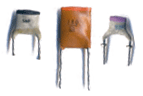
\includegraphics[scale=0.75]{Images/Code_couleur_derive_condensateurs.png}
	\caption{Code couleur dérive de la capacité
		\label{Code_couleur_derive_condensateurs}}
\end{figure}

L'unique bague de couleur au sommet des condensateurs céramiques code la dérive de la tolérance. Sur la figure \ref{Code_couleur_derive_condensateurs}, les condensateurs céramiques ont respectivement une dérive de 0 ppm/°C, -150 ppm/°C et -750 ppm/°C (de gauche à droite).

\paragraph{Codification \ac{EIA} condensateurs céramique classe II et supérieur}

Ce code indique la variation maximale de la capacité à l'intérieur de la plage de température. La capacité de référence est celle mesurée à 25°C. Voir le tableau \ref{Codification_EIA_condensateurs_céramique_classe_II}.

\begin{table}[H]
	\centering
		\begin{tabular}{|l|l||l|l||l|l|}\hline
				1\ier{} symbole & Température & 2\ieme{} symbole & Température & 3\ieme{} symbole & Variation max. de la\\
				(lettre) & minimale & (chiffre) & maximale & (lettre) & capacité sur la plage\\
				 & & & & & de température\\\hline\hline
				Z	& 10°C & 2 & 45°C & A & +1,0\%\\\hline
				Y	& -30°C & 4 & 65°C & B & $\pm$1,5\%\\\hline
				X	& -55°C & 5 & 85°C & C & $\pm$2,2\%\\\hline
				 & & 6 & 105°C & D & $\pm$3,3\%\\\hline
				 & & 7 & 125°C & E & $\pm$4,7\%\\\hline
				 & & & & F & $\pm$7,5\%\\\hline
				 & & & & P & $\pm$10\%\\\hline
				 & & & & R & $\pm$15\%\\\hline
				 & & & & S & $\pm$22\%\\\hline
				 & & & & T & +22\%, -33\%\\\hline
				 & & & & U & +22\%, -56\%\\\hline
				 & & & & V & +22\%, -82\%\\\hline
		\end{tabular}
	\caption{Codification \ac{EIA} condensateurs céramique classe II
		\label{Codification_EIA_condensateurs_céramique_classe_II}}
\end{table}

\subsubsection{Codification couleur des condensateurs céramique et plastique}

Le marquage à l'aide de couleurs sur les condensateurs est passé en désuétude, et ne se trouve plus que sur certains anciens condensateurs. Ce codage ne sera donc pas détaillé ici.

\subsubsection{Codification des condensateurs au mica}

\paragraph{Code \ac{EIA}}

Ce code est facilement identifiable car il commence par la lettre \og{}R\fg{}. Il se lit comme suit :

\begin{itemize}
	\item \textbf{R} : préfixe \ac{EIA} ;
	\item \textbf{CM/DM} : forme du composant (moulé/plongé) ;
	\item \textbf{XX} : nombre codant la taille du composant ;
	\item \textbf{X} : dérive de la capacité et coefficient de la température (voir tableau \ref{Derive_capacite_et_temperature_code_EIA}) ;
	\item \textbf{XXX} : valeur sur 3 chiffres (le 3\ieme{} chiffre étant le multiplicateur, correspondant au nombre de 0 à ajouter, la valeur étant exprimée en pico-farads) ;
	\item (\textbf{R}) : point décimal (facultatif) ;
	\item \textbf{X} : lettre codant la tolérance (voir tableau \ref{Lettre_de_tolerance}) ;
	\item \textbf{X} : chiffre indiquant la tension de service, en centaines de volt ;
	\item \textbf{X} : lettre indiquant la gamme de température (voir tableau \ref{Gamme_de_temperature_code_EIA}) ;
	\item \textbf{S/C} : connexions droites/pliées.
\end{itemize}

\begin{table}[H]
	\centering
		\begin{tabular}{|l|l|l|}\hline
				Lettre & Dérive max. en capacité & Coefficient de température\\\hline\hline
				B	& Non spécifié & Non spécifié\\\hline
				C	& $\pm$(0,5\% + 0,1 pF) & $\pm$200 ppm/°C\\\hline
				D	& $\pm$(0,3\% + 0,1 pF) & $\pm$100 ppm/°C\\\hline
				E	& $\pm$(0,1\% + 0,1 pF) & -20 à +100 ppm/°C\\\hline
				F	& $\pm$(0,05\% + 0,1 pF) & -0 à +70 ppm/°C\\\hline
		\end{tabular}
	\caption{Dérive capacité et température, code \ac{EIA}
		\label{Derive_capacite_et_temperature_code_EIA}}
\end{table}

\begin{table}[H]
	\centering
		\begin{tabular}{|l|l|}\hline
				Lettre & Gamme de température\\\hline\hline
				M	& -55 à 70°C\\\hline
				N	& -55 à 85°C\\\hline
				O	& -55 à 125°C\\\hline
				P	& -55 à 150°C\\\hline
		\end{tabular}
	\caption{Gamme de température, code \ac{EIA}
		\label{Gamme_de_temperature_code_EIA}}
\end{table}

Exemple, lecture de \og{}RCM05E391RJ5OS\fg{} :

\begin{itemize}
	\item \textbf{R} : préfixe \ac{EIA} ;
	\item \textbf{CM05} : forme et taille du composant ;
	\item \textbf{E} : dérive de capacité de $\pm$(0,1\% + 0,1 pF) et coefficient de température de -20 à +100 ppm/°C ;
	\item \textbf{39} : capacité (1\ier{} et 2\ieme{} chiffres significatifs) ;
	\item \textbf{1} : capacité (nombre de zéros à ajouter aux chiffres ci-dessus) ;
	\item \textbf{R} : point décimal (facultatif).\\
	La capacité du condensateur est donc ici de 390 pF ;
	\item \textbf{J} : tolérance de 5\% ;
	\item \textbf{5} : tension de service de 500 V ;
	\item \textbf{O} : température de -55 à +125°C ;
	\item \textbf{S} : connexions droites.
\end{itemize}

\paragraph{Military code}

Ce code est destiné aux composants à usage militaire. Il est proche du code \ac{EIA}, qui l'utilise en partie, mais ne commence pas par la lettre \og{}R\fg{}. Les principales différences concernent la tension de service et la résistance aux vibrations.

\paragraph{Marquage par points de couleur}

Ce marquage n'est plus guère utilisé est ne sera pas détaillé ici.

\subsection{Les condensateurs de découplage}

% http://bicmos.chez-alice.fr/questionMOS.html#30

On parle également couramment, par abus de langage, de capacités de découplage.

Lors de la transition d'un circuit logique (passage d'une broche d'un état à l'autre), un courant transitoire $\Delta$I circule dans le circuit d'alimentation (voir figure  \ref{Alimentation_circuit_sans_capa_decouplage}). Cela provoque une chute de tension aux bornes de son inductance équivalente, qui existe toujours, la ligne d'alimentation étant un fil, mais qui est généralement négligée. Cette chute de tension peut être relativement importante (plusieurs volts), au point de perturber le fonctionnement des circuits logiques. De plus, l'inductance du circuit d'alimentation a tendance à s'opposer aux brusques variations de courant ce qui a pour conséquence un allongement du temps de transition du circuit logique, comme illustré figure \ref{Tensions_circuit_sans_decouplage}.

\begin{figure}[H]
	\centering
	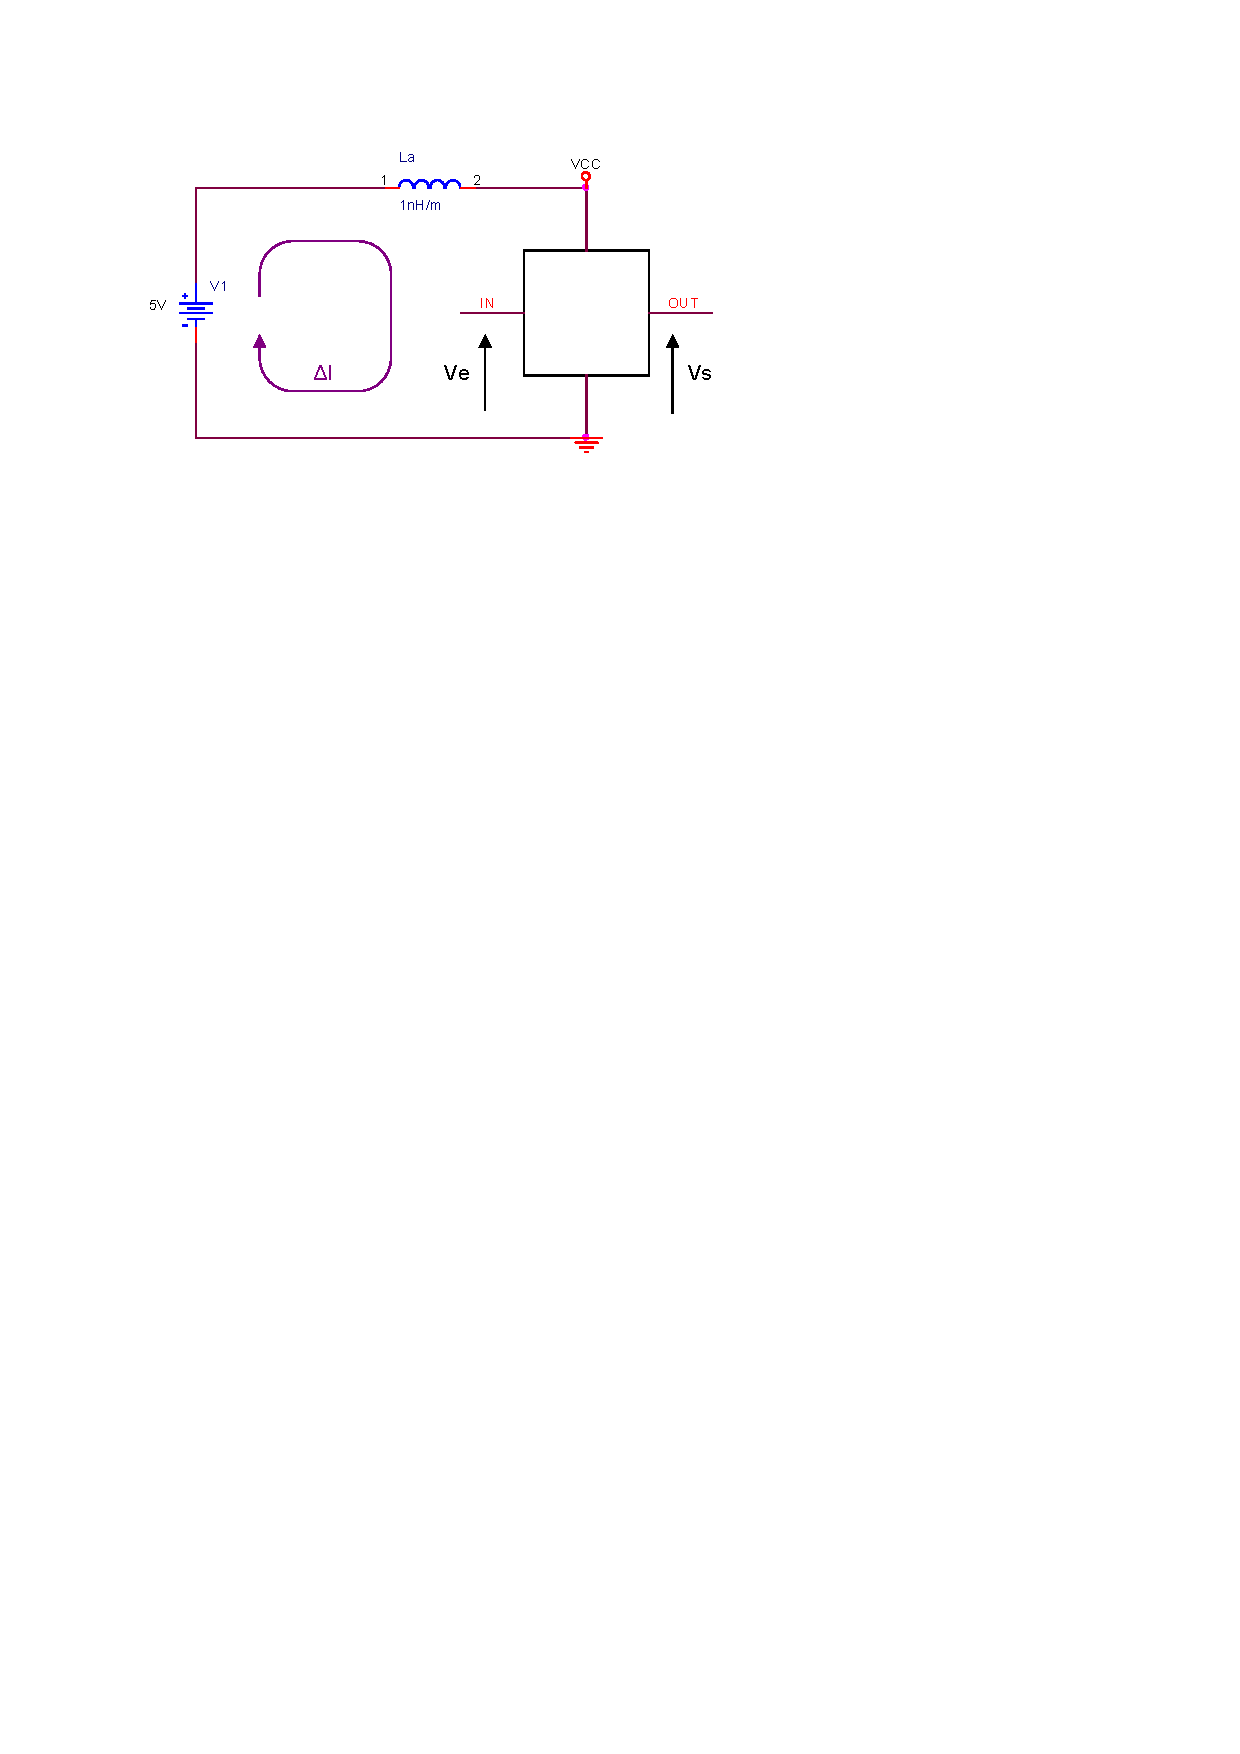
\includegraphics[scale=1.00]{Images/Alimentation_circuit_sans_capa_decouplage}
	\caption{Alimentation d'un circuit sans capacité de découplage
		\label{Alimentation_circuit_sans_capa_decouplage}}
\end{figure}

\begin{figure}[H]
	\centering
	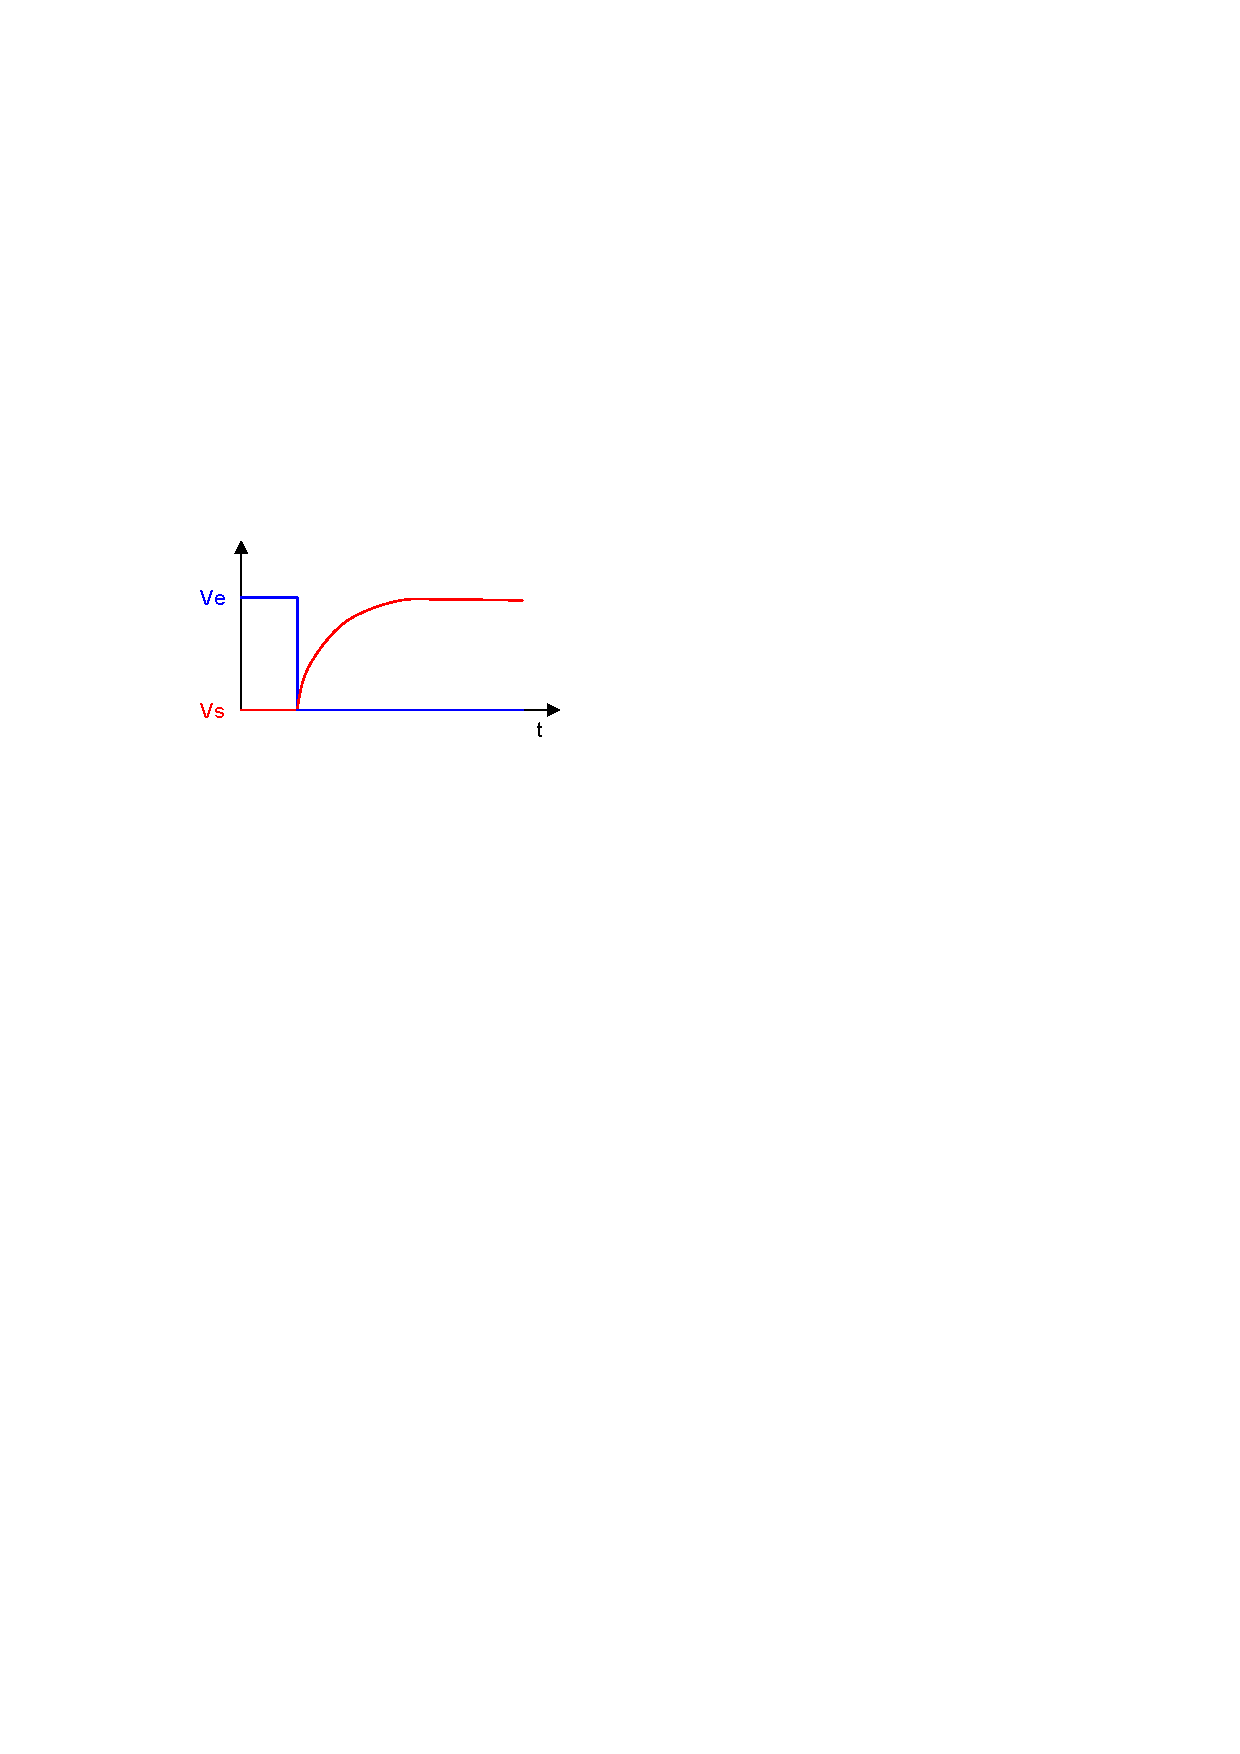
\includegraphics[scale=1.00]{Images/Tensions_circuit_sans_decouplage}
	\caption{Tensions aux bornes d'un circuit logique sans découplage
		\label{Tensions_circuit_sans_decouplage}}
\end{figure}

L'ajout d'une capacité de découplage aux bornes de l'alimentation du circuit logique permet de limiter ces phénomènes, en agissant comme une source locale de charge et en diminuant l'impédance équivalente, sur la figure \ref{Alimentation_circuit_avec_capa_decouplage}. Elle joue alors le rôle de stabilisateur de tension et contribue à réduire la boucle de circulation du courant transitoire $\Delta$I, également à l'origine de rayonnement électromagnétique.

\begin{figure}[H]
	\centering
	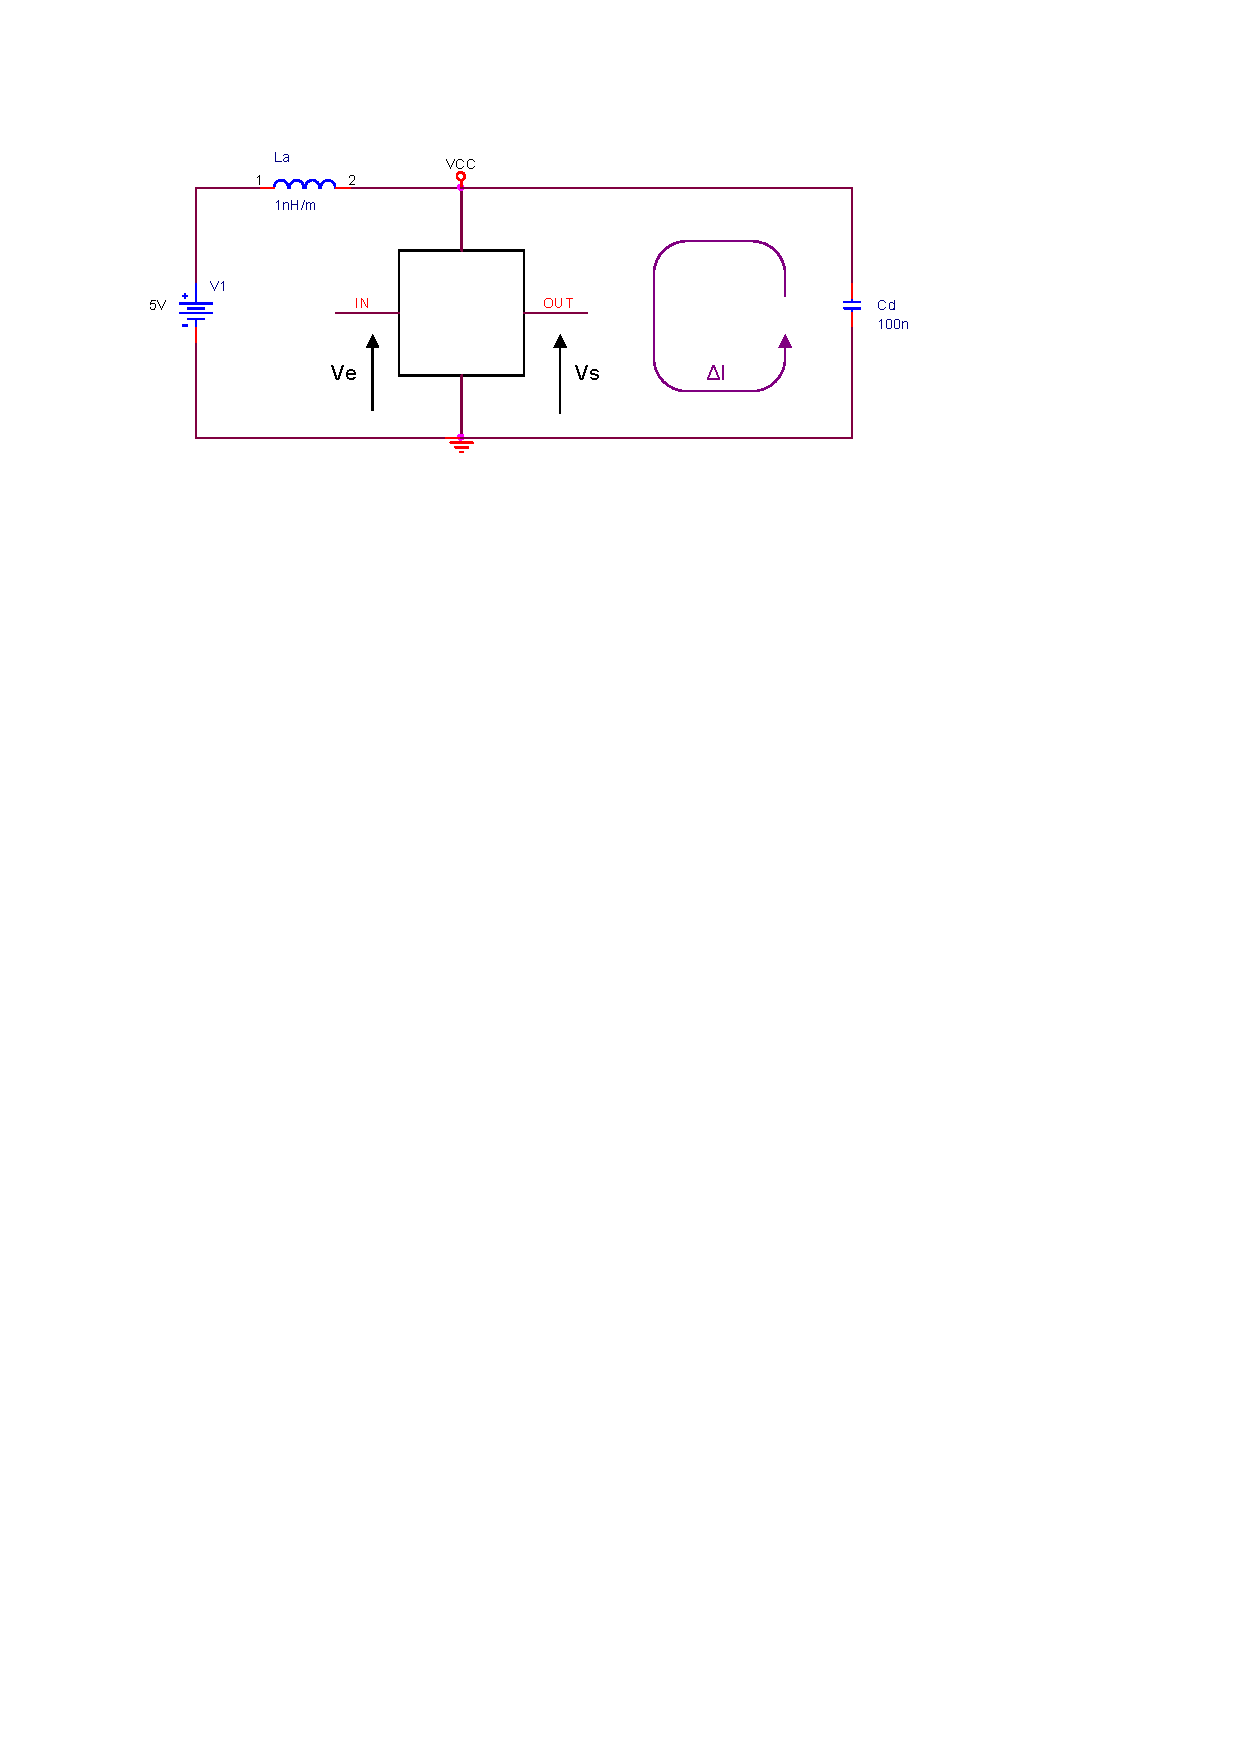
\includegraphics[scale=1.00]{Images/Alimentation_circuit_avec_capa_decouplage}
	\caption{Alimentation d'un circuit avec capacité de découplage
		\label{Alimentation_circuit_avec_capa_decouplage}}
\end{figure}

\begin{figure}[H]
	\centering
	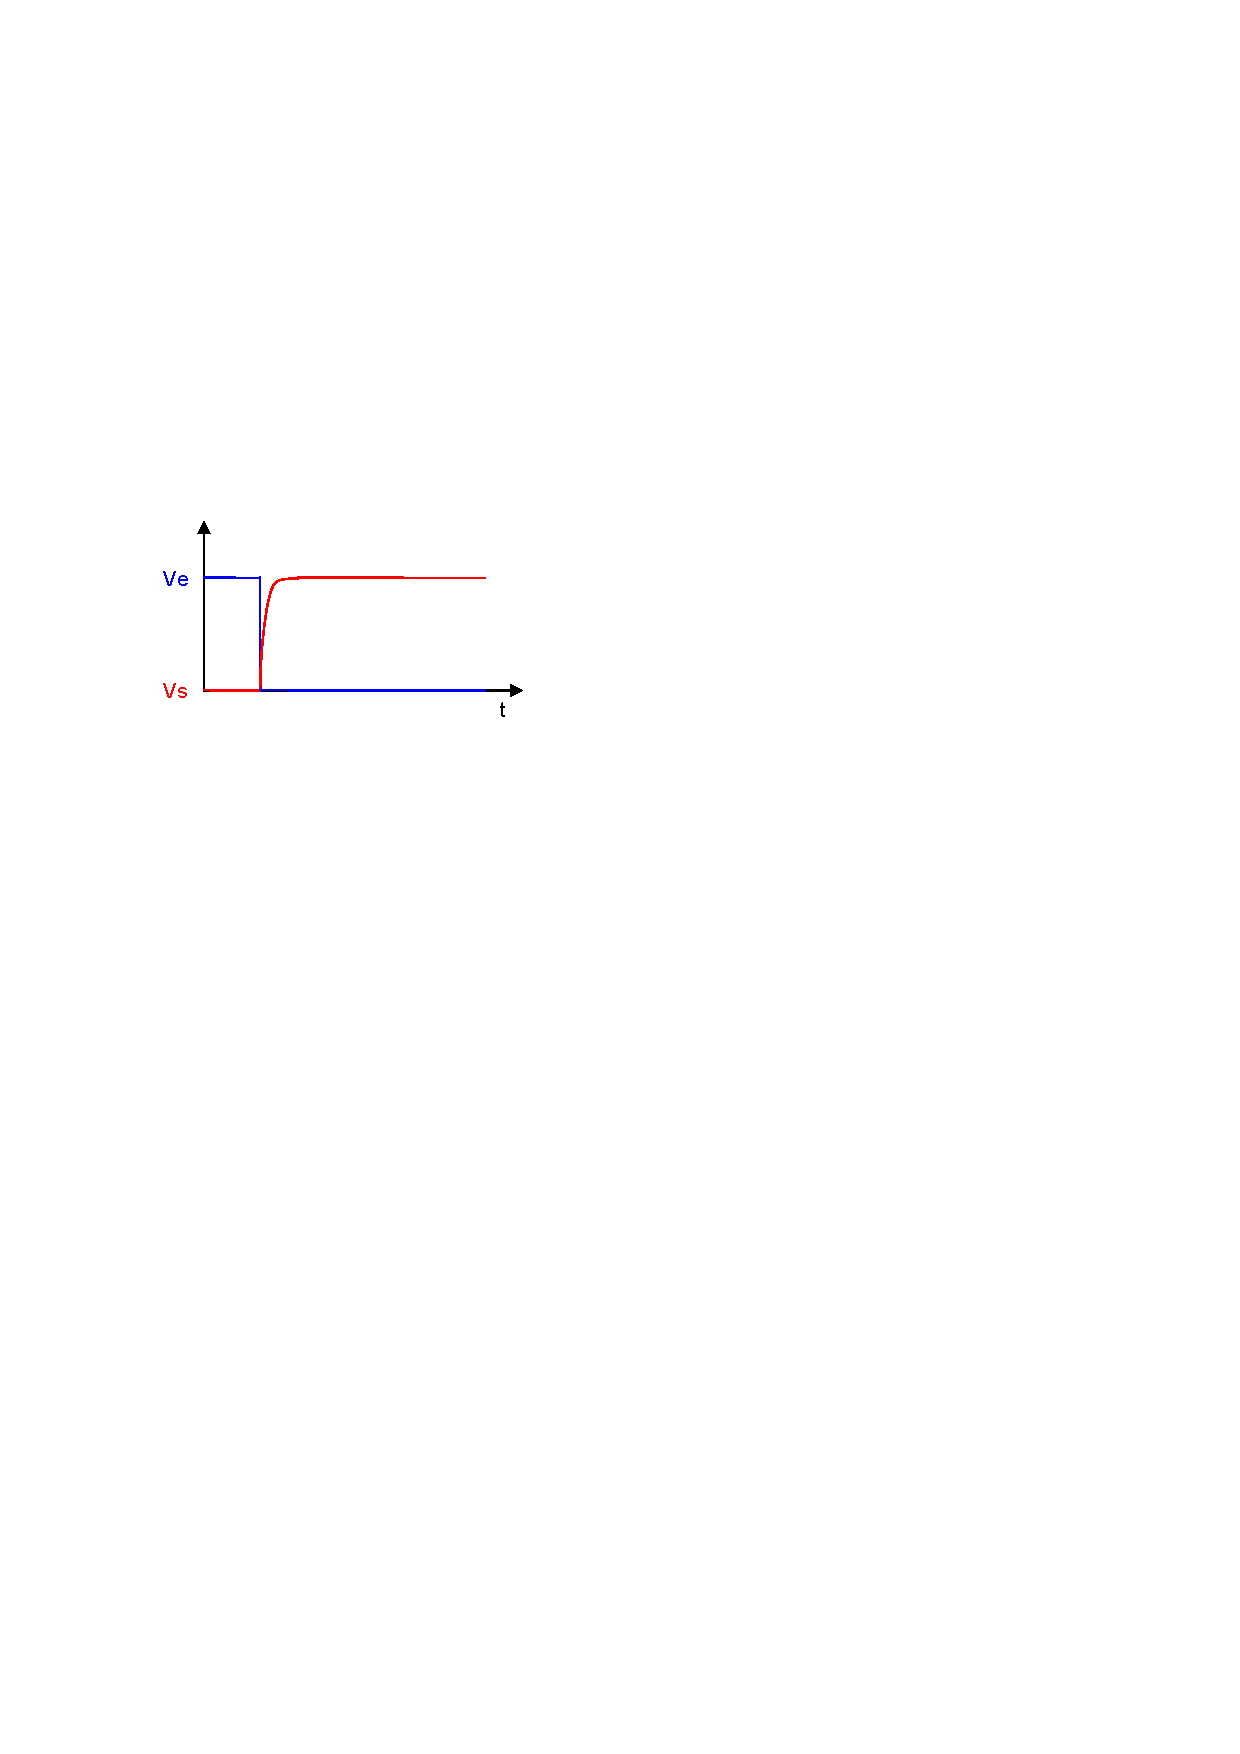
\includegraphics[scale=1.00]{Images/Tensions_circuit_avec_decouplage}
	\caption{Tensions aux bornes d'un circuit logique avec découplage
		\label{Tensions_circuit_avec_decouplage}}
\end{figure}

Le condensateur de découplage va en plus permettre une commutation rapide des circuits logiques en fournissant l'énergie requise par le brusque appel de courant $\Delta$I lors de la commutation (figure \ref{Tensions_circuit_avec_decouplage}).

On comprend que pour qu'une capacité de découplage soit efficace, il faut la placer au plus prêt de l'alimentation du circuit logique, afin d'avoir l'inductance la plus faible possible entre l'alimentation du circuit logique et le condensateur. Ainsi, il est clair que chaque circuit logique doit avoir sa propre capacité de découplage.

Une valeur de capacité de découplage couramment utilisée est 100 nF.

\subsection{Les condensateurs de lissage}

Un condensateur de lissage (en anglais \og{}smoothing capacitor\fg{}), comme son nom l'indique, \og{}lisse\fg{} la tension, c'est-à-dire qu'il agit comme un réservoir, permettant de compenser les variations de tension. Un condensateur de lissage est ajouté sur l'alimentation, en parallèle à une charge, figure \ref{Condensateur_de_lissage_schema}.

\begin{figure}[H]
	\centering
	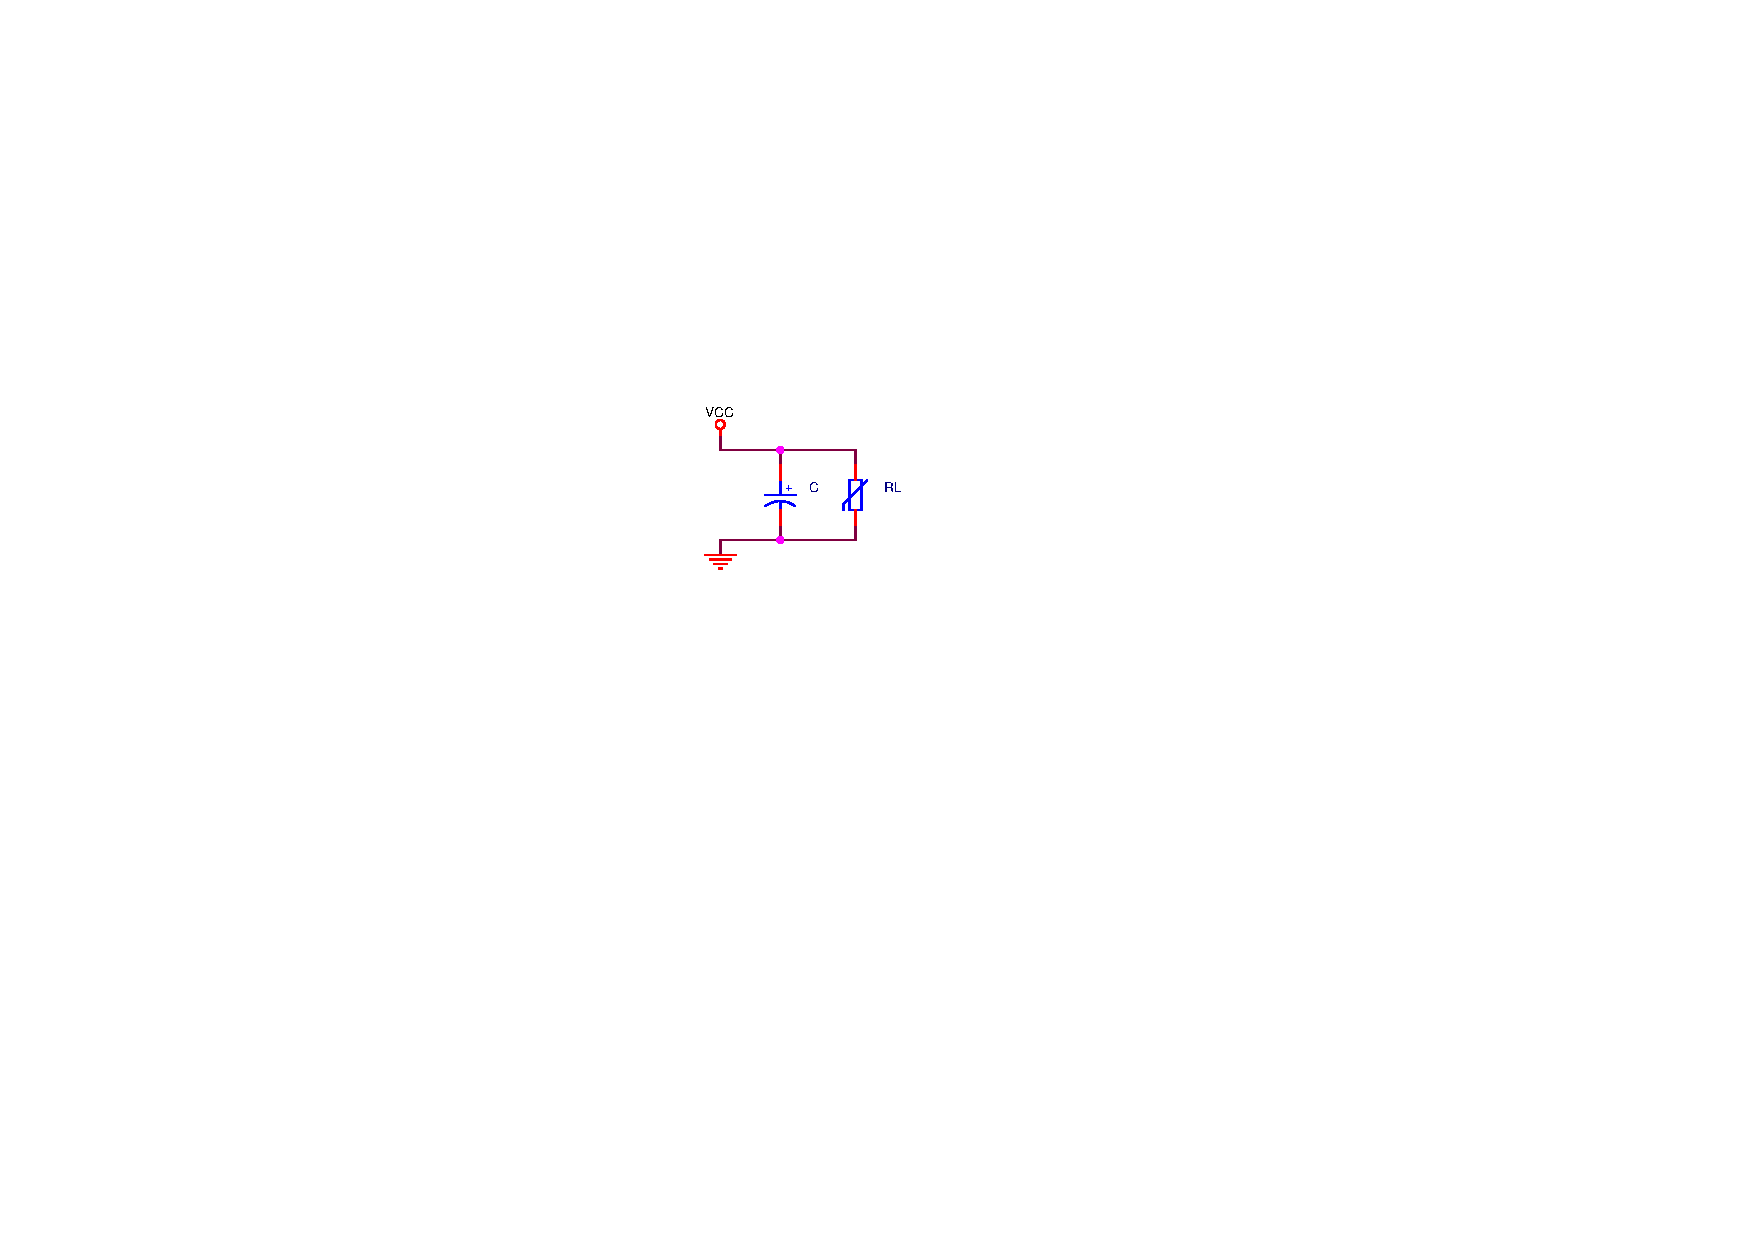
\includegraphics[scale=1.00]{Images/Condensateur_de_lissage_schema}
	\caption{Mise en place d'un condensateur de lissage
		\label{Condensateur_de_lissage_schema}}
\end{figure}

La figure \ref{Condensateur_de_lissage} montre comment la présence d'un condensateur, de capacité relativement importante, lisse la tension : la courbe 1 représente la tension d'alimentation VCC sans condensateur de lissage et la courbe 2 la tension aux bornes du condensateur.

\begin{figure}[H]
	\centering
	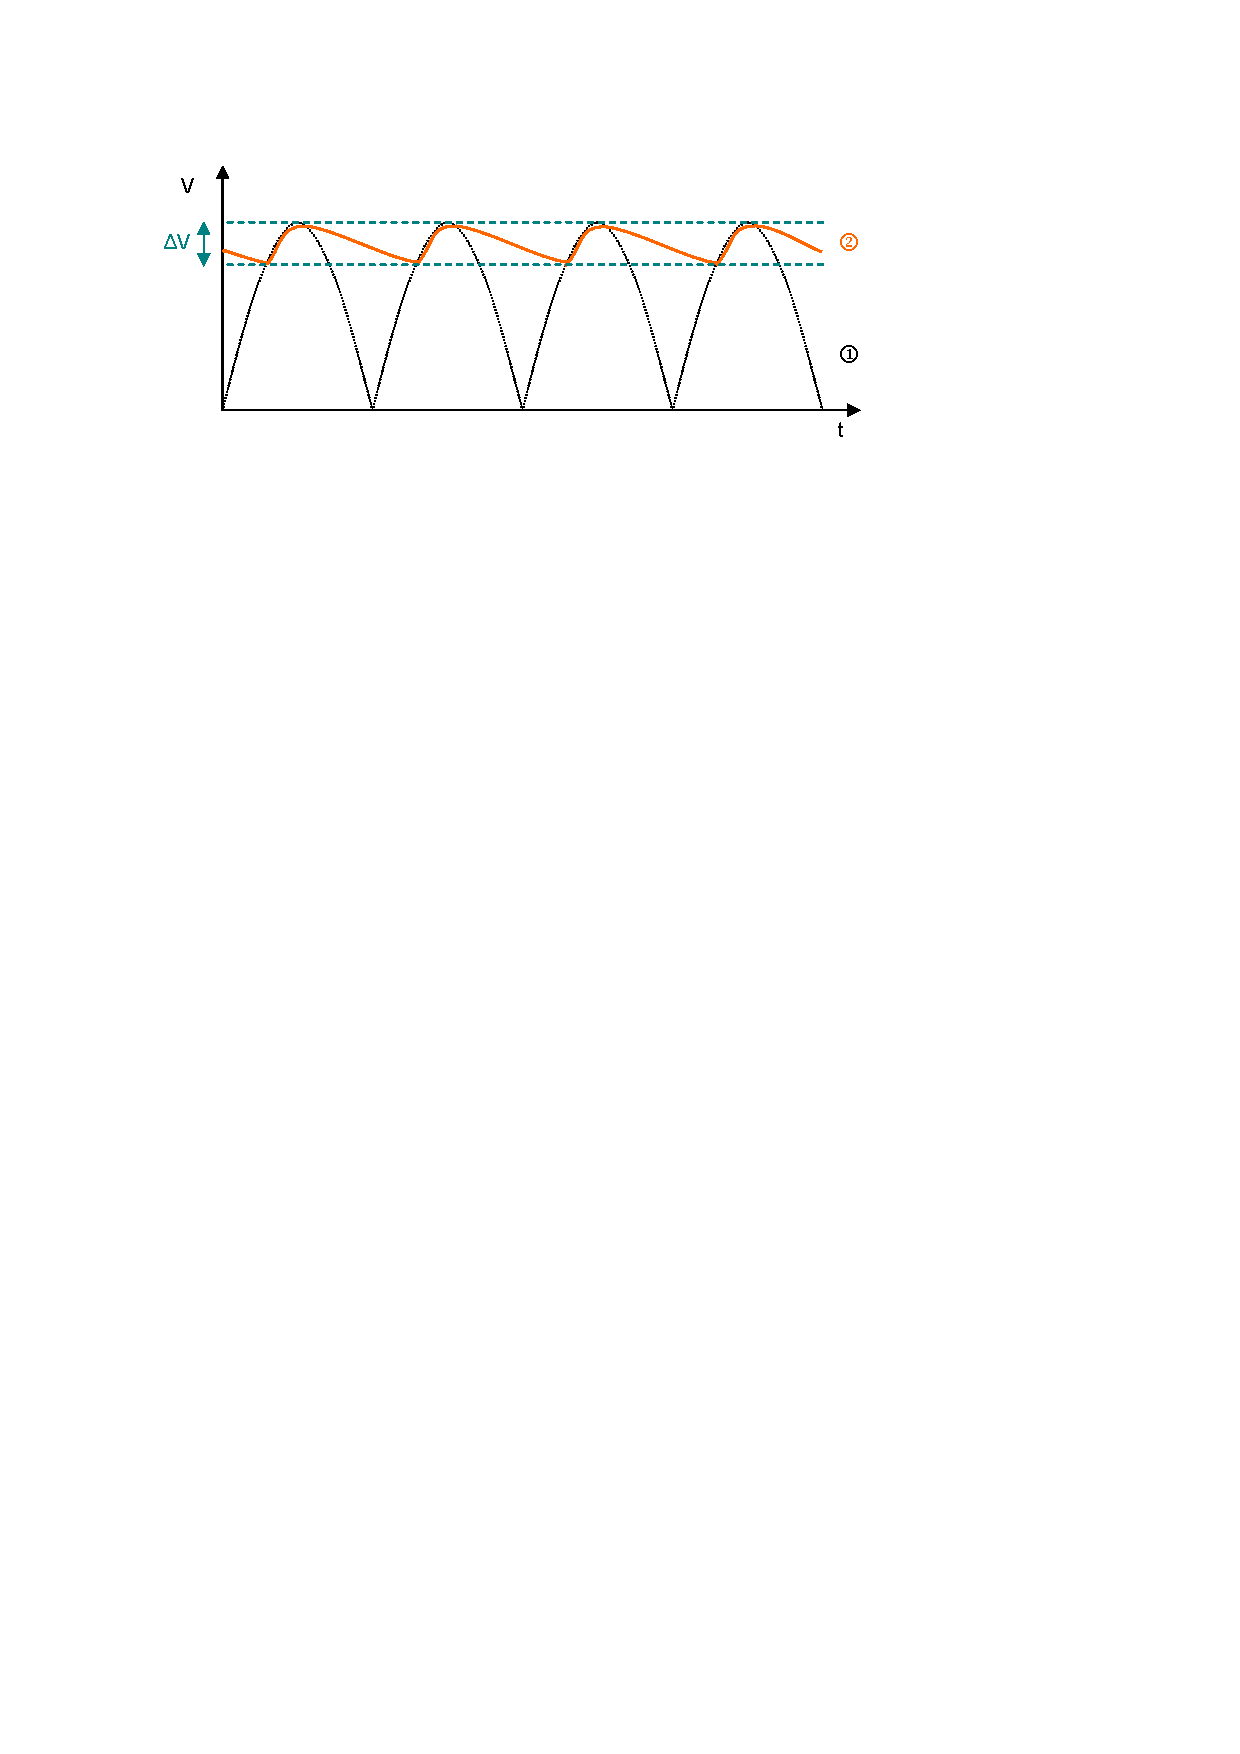
\includegraphics[scale=1.00]{Images/Condensateur_de_lissage}
	\caption{Lissage de la tension avec un condensateur de lissage
		\label{Condensateur_de_lissage}}
\end{figure}

La capacité C est donnée par la formule suivante :

\[C = \frac{I}{\Delta{}V \times f}\]

où

\begin{itemize}
	\item $I$ est le courant provenant de l'alimentation ;
	\item $\Delta{}V$ est la variation maximale de tension que l'on veut avoir ;
	\item $f$ est la fréquence du signal, ou l'ordre de grandeur de la fréquence de fluctuation du signal, fluctuations qui peuvent être dues aux transitions des circuits logiques (voir les condensateurs de découplage).
\end{itemize}

Si l'on ne veut pas que la variation de tension n'excède les 10\% de la tension maximale, C est donné par :

\[C = \frac{I}{0,1 \times V_{max} \times f}\]

Si $V_{max}$ = 5 V, $I$ = 100 mA et $f$ $\approx$ 1 MHz, on trouve C $\approx$ 200 nF, ce qui est bien l'ordre de grandeur des capacités de découplage étudiées précédemment.

Si $V_{max}$ = 12 V, $I$ = 0,5 A et $f$ $\approx$ 100 Hz, on trouve C $\approx$ 4\,200 $\mu$F, qui conviendrait pour stabiliser la tension aux bornes de batteries par exemple, avant un régulateur de tension. Évidemment, le condensateur ne compensera toutefois pas la lente baisse de tension de la batterie dû à sa décharge.

Ces valeurs de capacité ne sont que des ordres de grandeur, mais permettent de mieux appréhender pourquoi l'on met tel capacité à tel endroit, notamment au niveau de l'alimentation.

Maintenant vous pourriez vous dire que qui peut le plus, peut le moins. Ainsi, un condensateur de capacité élevée devrait en principe également stabiliser des variations de tension très rapides. Mais en pratique ce n'est pas le cas ! Pourquoi ? Car les condensateurs de grosse capacité sont forcément des condensateurs électrochimiques, qui sont caractérisés par une certaine inertie. Leur temps de réaction est en fait trop élevé pour qu'ils puissent suivre des fluctuations rapides de tension, ce qui les rend inefficaces dans les hautes fréquences. C'est pourquoi on utilise en parallèle à ceux-ci des condensateurs de capacité plus faible, généralement des céramiques, pour stabiliser les hautes fréquences, comme illustré par la figure \ref{Condensateurs_stabilisation}.

\begin{figure}[H]
	\centering
	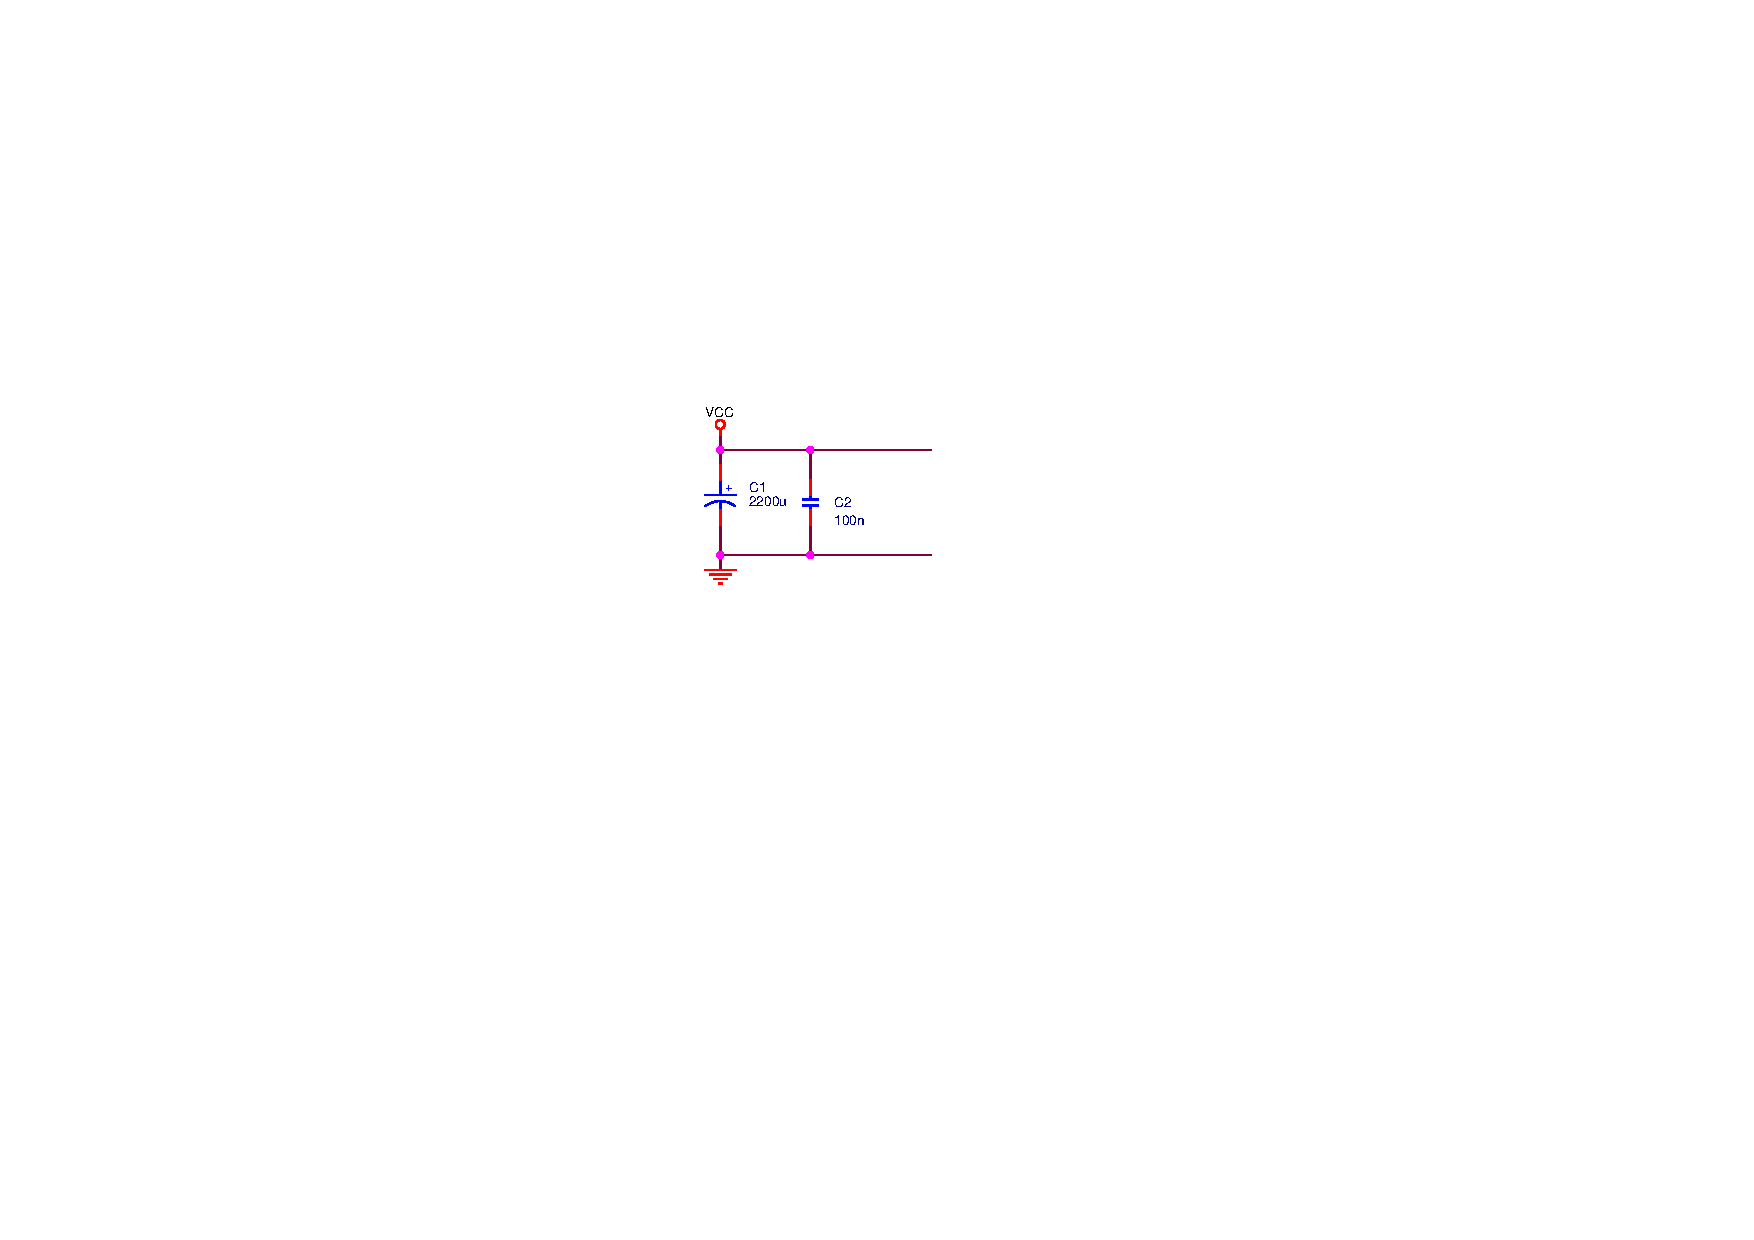
\includegraphics[scale=1.00]{Images/Condensateurs_stabilisation}
	\caption{Stabilisation de l'alimentation (classique)
		\label{Condensateurs_stabilisation}}
\end{figure}

\section{Les diodes}

\subsection{Repérage anode - cathode}

\begin{figure}[H]
	\centering
	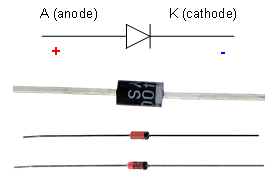
\includegraphics[scale=0.75]{Images/Diodes_sens.png}
	\caption{Repérage de l'anode et de la cathode des diodes
		\label{Diodes_sens}}
\end{figure}

La cathode est généralement repérée par une bague. Lorsqu'il y a plusieurs bagues de couleur sur la diode, c'est la bague la plus grosse qui repère la cathode, ou alors les bagues sont plus proches de la cathode que de l'anode.

\subsection{Marquage des diodes}

\subsubsection{Le code JEDEC}

\begin{figure}[H]
\begin{minipage}[c]{.45\linewidth}
	\flushright
		\begin{tabular}{|l|l|}\hline
			Code couleur & Valeur\\\hline\hline
			\cellcolor{black}\color{white}Noir & 0\\\hline
			\cellcolor{marron}\color{white}Marron & 1\\\hline
			\cellcolor{red}Rouge & 2\\\hline
			\cellcolor{orange}Orange & 3\\\hline
			\cellcolor{yellow}Jaune & 4\\\hline
			\cellcolor{green}Vert & 5\\\hline
			\cellcolor{blue}\color{white}Bleu & 6\\\hline
			\cellcolor{purple}Violet & 7\\\hline
			\cellcolor{gray}Gris & 8\\\hline
			\cellcolor{white}Blanc & 9\\\hline
		\end{tabular}
	\end{minipage} \hfill
	\begin{minipage}[c]{.45\linewidth}
		\flushleft
		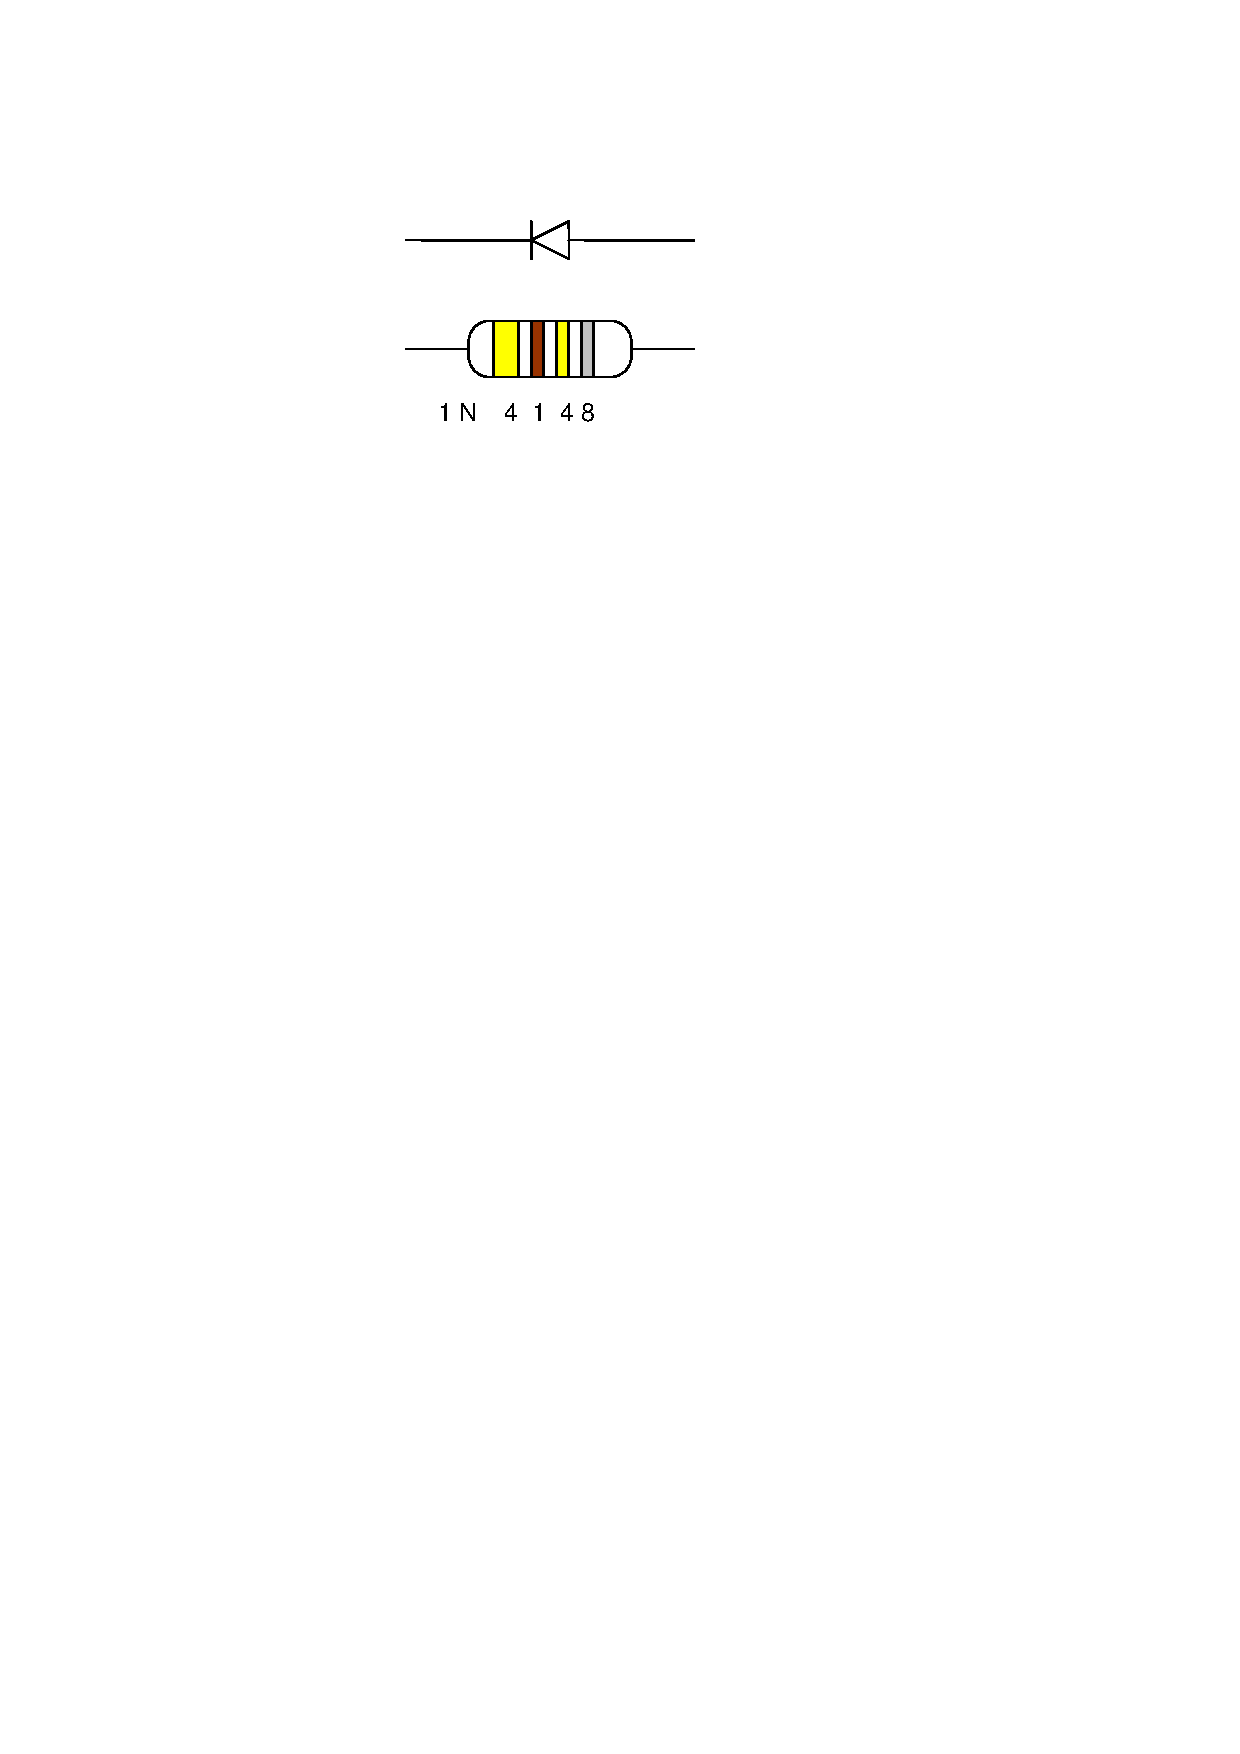
\includegraphics[scale=1.00]{Images/Code_JEDEC_diodes}
	\end{minipage}	
	\caption{Le codage JEDEC
		\label{Code_JEDEC_diodes}}
\end{figure}

\begin{figure}[H]
	\centering
	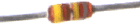
\includegraphics[scale=0.75]{Images/Diode_1N4148_JEDEC.png}
	\caption{Une diode 1N4148 avec le codage JEDEC
		\label{Diode_1N4148_JEDEC}}
\end{figure}

\section{Les circuits intégrés}

\subsection{Les familles de circuits logiques}

Les deux technologies les plus connues pour les circuits intégrés sont les technologies \ac{TTL} et \ac{CMOS}. Actuellement, la technologie \ac{CMOS} est la plus utilisée au détriment de la technologie \ac{TTL}.

\[\underbrace{XX}_{\textrm{Identifiant constructeur}} \overbrace{74/54}^{\stackrel{\textrm{74 : série commerciale (0° à 70°C)}}{\textrm{54 : série militaire (-55° à 125°C)}}} \underbrace{XXX}_{\textrm{Famille techno.}} \overbrace{XXX}^{\textrm{Référence fonction}} \underbrace{XXX}_{\textrm{Packaging}}\]

\begin{figure}[H]
	\centering
	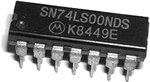
\includegraphics[scale=0.75]{Images/Photo_74LS00.png}
	\caption{Photo d'un 74LS00
		\label{Photo_74LS00}}
\end{figure}

On lit sur la figure \ref{Photo_74LS00} :
\begin{itemize}
	\item Identifiant constructeur : SN. Série standard propre à Texas Instruments ;
	\item Série : 74 - série commerciale ;
	\item Famille technologique : LS. Il s'agit donc d'un composant de technologie \ac{TTL}, le LS signifiant Low-power Schottky (voir tableau \ref{Liste_des_sous_familles_TTL}) ;
	\item Référence fonction : 00. Ce numéro permet d'identifier la fonction réalisé par le circuit logique. Ici il s'agit d'un  quadruple NAND ;
	\item Type de boitier : NDS. Identifie le packaging du composant (se rapporter à la datasheet du composant pour plus de détails).
\end{itemize}

\subsubsection{Technologie TTL}

Désignations et sous familles

\begin{table}[H]
	\centering
		\begin{tabular}{|l|c|c|c|c|c|}\hline
				Sous famille (séries commerciales) & Tension d'alim. & Temps prop. & Conso. & Fréq. max.\\\hline\hline
				74* & \multirow{8}{*}{5 V $\pm$ 5\%} & 10 ns & 10 mW & 25 MHz\\\cline{1-1}\cline{3-5}
				74L (Low-power)* & & 33 ns & 1 mW & 5 MHz\\\cline{1-1}\cline{3-5}
				74H (High-speed)* & & 6 ns & 22 mW & \\\cline{1-1}\cline{3-5}
				74S (Schottky) & & 3 ns & 19 mW & 75 MHz\\\cline{1-1}\cline{3-5}
				74LS (Low-power Schottky) & & 9 ns & 2 mW & 30 MHz\\\cline{1-1}\cline{3-5}
				74AS (Advanced Schottky) & & 7 ns & 5 mW & \\\cline{1-1}\cline{3-5}
				74ALS (Advanced Low-power Schottky) & & 7 ns & 5 mW & \\\cline{1-1}\cline{3-5}
				74F(AST) (Fast (Advanced Schottky)) & & 6 ns & 5 mW & 100 MHz\\\hline
		\end{tabular}
		\caption{Liste des sous familles \ac{TTL}
			\label{Liste_des_sous_familles_TTL}}
\end{table}
* Devenue aujourd'hui partiellement, voir totalement, obsolète

\subsubsection{Technologie CMOS}

Désignations et sous familles

\begin{table}[H]
	\centering
		\begin{tabular}{|l|c|c|c|c|c|}\hline
				Sous famille (séries commerciales) & Tension d'alim. & Temps prop. & Conso. & Fréq. max.\\\hline\hline
				4000* & 3 à 15 V & 40 ns & 0,1 mW & 12 MHz\\\hline
				74C (\ac{CMOS} pin-compatible with \ac{TTL})* & 5 V $\pm$ 10\% & 50 ns & 0,1 mW & 50 MHz\\\hline
				74HC (High-speed C) & 2 à 6 V & 18 ns & 0,06 mW & 50 MHz\\\hline
				74HCT (HC \ac{TTL} compatible) & 5 V $\pm$ 10\% & 18 ns & 0,06 mW & 50 MHz\\\hline
				74AC (Advanced C) & 2 à 6 V & 5 ns & 0,1 mW & 70 MHz\\\hline
				74ACT (AC \ac{TTL} compatible) & 6 V & 5 ns & 0,1 mW & 70 MHz\\\hline
				74AHC (Advanced HC) & 2 à 6 V & 5 ns & 0,1 mW & 70 MHz\\\hline
				74AHCT (Advanced HCT) & 6 V & 5 ns & 0,1 mW & 70 MHz\\\hline
				74FCT (Fast \ac{CMOS} \ac{TTL} compatible) & 6 V & 5 ns & 0,1 mW & 70 MHz\\\hline
		\end{tabular}
	\caption{Liste des sous familles \ac{CMOS}
		\label{Liste_des_sous_familles_CMOS}}
\end{table}
* Devenue aujourd'hui partiellement, voir totalement, obsolète

La liste des sous familles est loin d'être exhaustive !

\subsection{Compatibilité TTL - CMOS}

Il est toujours préférable de ne pas mélanger les technologies sur un même circuit électronique, et travailler exclusivement avec du \ac{CMOS} ou avec du \ac{TTL}, dans la mesure où l'on trouve généralement des équivalents dans chaque technologie.

Si toutefois nous sommes amené à mélanger plusieurs technologies, il faut être prudent et s'assurer entre autre que les tensions de seuil sont compatibles d'une technologie à l'autre (mais cela n'est pas forcément suffisant).

\subsubsection{TTL vers CMOS}

Il n'y a pas compatibilité sauf si la porte \ac{CMOS} est du type \ac{TTL} compatible (typiquement, les 74HCT) : la tension de sortie minimale au niveau haut des circuits \ac{TTL}, de 2,4 V, n'est pas compatible avec la tension minimale d'entrée des circuits \ac{CMOS}, qui vaut 3,5 V. Sinon, il est possible d'assurer la compatibilité en ajoutant une résistance de tirage entre la sortie du \ac{TTL} et l'entrée du \ac{CMOS}, comme sur la figure \ref{TTL_vers_CMOS} (ce qui, comme nous l'avons vu, n'est pas nécessaire entre deux composants de la même technologie). Il est également possible d'intercaler une porte \ac{TTL} compatible entre le \ac{TTL} et le \ac{CMOS}.

\begin{figure}[H]
	\centering
	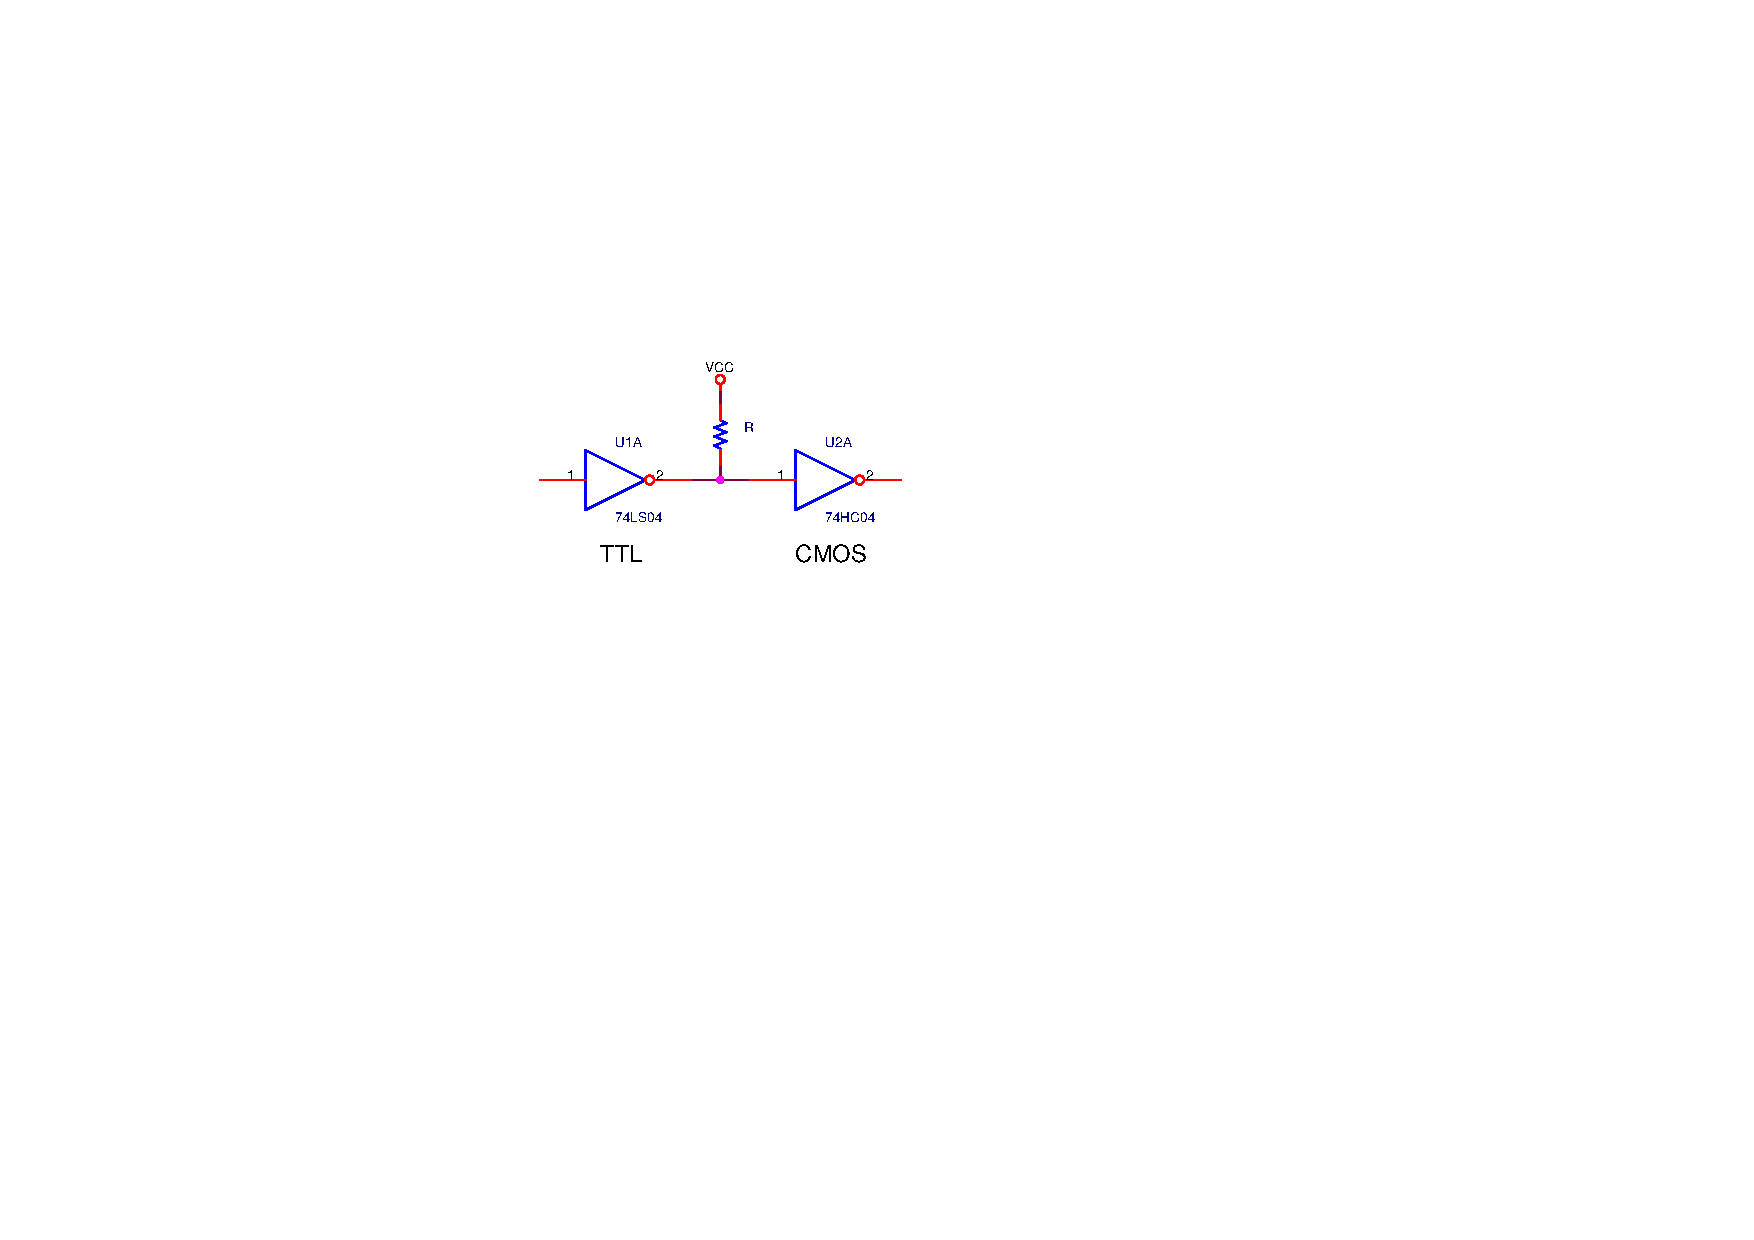
\includegraphics[scale=1.00]{Images/TTL_vers_CMOS}
	\caption{TTL vers CMOS avec résistance de tirage
		\label{TTL_vers_CMOS}}
\end{figure}

On doit avoir

\[R > \frac{(VCC - V_{OL_{max}}^{^{TTL}})}{I_{OL}^{^{TTL}} - n \times I_{IL}^{^{CMOS}}} = \frac{(5 - 0,5)}{0,008 - n \times 0} \approx 600\ \Omega\]

où $n$ est le nombre d'entrées \ac{CMOS} connectés à la sortie \ac{TTL}. En pratique, une résistance de 1 à 10 k$\Omega$ convient.

\subsubsection{CMOS vers TTL}

Il y a compatibilité en règle générale.

\subsection{Les entrées inutilisées}

Si vous avez bien compris à quoi sert une résistance de tirage, vous savez qu'il ne faut jamais laisser de broche d'entrée d'un circuit logique en haute impédance. Une quantité très faible de charge peut provoquer le changement d'état de l'entrée, par exemple à l'approche d'un objet ou d'un doigt. De plus, la variation des charges au niveau de l'entrée risque de la mettre dans un état instable et la faire constamment basculer d'un état logique à l'autre, ce qui va provoquer des appels de courant sur le circuit d'alimentation perturbant les autres circuits logiques, et le composant va chauffer anormalement.

\subsection{L'électricité statique}

La plupart des circuits intégrés sont sensibles à l'électricité statique (particulièrement les \ac{CMOS}) et peuvent être endommagés en les manipulant, si vous les touchez avec vos doigt et que vous êtes chargé en électricité statique, provenant de vos habits par exemple. Les circuits sensibles à l'électricité statique sont généralement vendu dans des sachets antistatiques, comme ceux représentés figure \ref{Sachets_antistatiques}.

\begin{figure}[H]
	\centering
	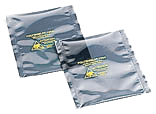
\includegraphics[scale=0.75]{Images/Sachets_antistatiques.png}
	\caption{Sachets antistatiques
		\label{Sachets_antistatiques}}
\end{figure}

Afin de garantir le bon état des circuits intégrés, il est important de les conserver dans leurs emballages antistatiques adaptés jusqu'à leur utilisation effective.

Il peut également être prudent de se décharger en électricité statique avant de les manipuler, en touchant un conducteur relié à la terre, comme une conduite d'eau en métal par exemple.

\section{Les PICs}

Avant toute chose, voici la documentation minimum dont vous aurez besoin pour apprendre à connaitre les PICs :

\begin{itemize}
	\item La datasheet du PIC (nous nous intéressons ici à la famille PIC18FXX2) \cite{PIC18FXX2} ;
	\item MPLAB C18 C Compiler Libraries (librairies disponibles en C pour les PICs) ;
	\item Éventuellement, un manuel de langage C à porté de main.
\end{itemize}

Logiciels nécessaires :

\begin{itemize}
	\item MPLAB \ac{IDE}\footnote{Téléchargeable gratuitement sur le site de Microchip : \url{http://www.microchip.com/}} (Integrated Development Environment) : environnement de développement en C ;
	\item MPLAB C18\footnote{\url{http://www.microchip.com/}} : compilateur C ;
	\item ICPROG\footnote{\url{http://www.ic-prog.com/}} : permet de transférer le programme compilé sur le PIC, via le programmateur.
\end{itemize}

\subsection{Installation de l'environnement de développement}

Pour mettre en place l'environnement de développement sur PC pour notre PIC, il y a donc trois logiciels à installer. Le mieux est d'installer dans l'ordre, MPLAB \ac{IDE}, MPLAB C18 (en prenant garde de ne pas mettre à jour les variables locales, nous le ferons manuellement plus tard) et ICPROG.

\subsubsection{Intégrer MPLAB C18 à MPLAB IDE}

Une fois MPLAB \ac{IDE} et MPLAB C18 installés, il faut configurer \ac{IDE} pour utiliser le compilateur C18. Pour se faire, voici la procédure à suivre, dans MPLAB \ac{IDE} :

\begin{enumerate}
	\item Ouvrir le menu \og{}Project\fg{} $\rightarrow$ \og{}Set Language Tool Locations\fg{} et développer la section \og{}Microchip C18 Toolsuite\fg{}.
		\begin{figure}[H]
			\centering
			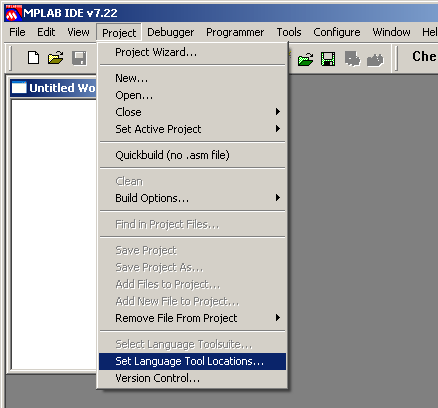
\includegraphics[scale=0.75]{Images/Le_logiciel_MPLAB_IDE.png}
			\caption{Le logiciel MPLAB \ac{IDE}
				\label{Le_logiciel_MPLAB_IDE}}
		\end{figure}
		On considère par la suite que le répertoire d'installation de MPLAB \ac{IDE} est\\
		{\ttfamily C:$\backslash$Program Files$\backslash$MPLAB IDE} et que celui du compilateur MPLAB C18 est\\
		{\ttfamily C:$\backslash$mcc18} ;
		\begin{figure}[H]
			\centering
			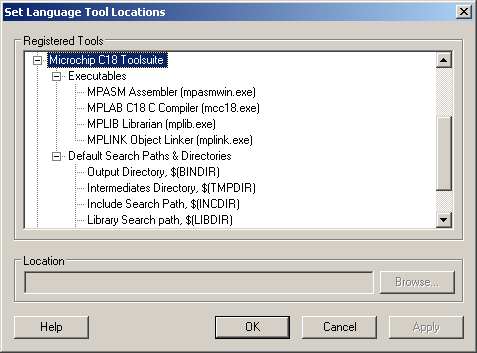
\includegraphics[scale=0.75]{Images/Set_Language_Tool_Locations.png}
			\caption{La boite de dialogue \og{}Set Language Tool Locations\fg{}
				\label{Set_Language_Tool_Locations}}
		\end{figure}
	\item Complétez alors les différentes lignes de cette section comme suit :
		\begin{itemize}
			\item MPASM Assembler (mpasmwin.exe) :\\
			{\ttfamily C:$\backslash$Program Files$\backslash$MPLAB IDE$\backslash$MPASM Suite$\backslash$MPASMWIN.EXE} ;
			\item MPLAB C18 C Compiler (mcc18.exe) : {\ttfamily C:$\backslash$mcc18$\backslash$bin$\backslash$mcc18.exe} ;
			\item MPLIB Librarian (mplib.exe) : {\ttfamily C:$\backslash$mcc18$\backslash$bin$\backslash$mplib.exe} ;
			\item MPLINK Object Linker (mplink.exe) : {\ttfamily C:$\backslash$mcc18$\backslash$bin$\backslash$mplink.exe} ;
			\item Include Search Path, \$(INCDIR) : {\ttfamily C:$\backslash$mcc18$\backslash$h} ;
			\item Library Search Path, \$(LIBDIR) : {\ttfamily C:$\backslash$mcc18$\backslash$lib} ;
			\item Linker-Script Search Path, \$(LKRDIR) : {\ttfamily C:$\backslash$mcc18$\backslash$lkr}.
		\end{itemize}
\end{enumerate}

Désormais, \ac{IDE} sait où trouver les librairies et le compilateur.

\subsubsection{Créer un projet avec MPLAB IDE}

\begin{enumerate}
	\item Dans MPLAB \ac{IDE}, ouvrir le menu \og{}Project\fg{} $\rightarrow$ \og{}New\fg{}. Donner un nom et un répertoire au projet ;
		\begin{figure}[H]
			\centering
			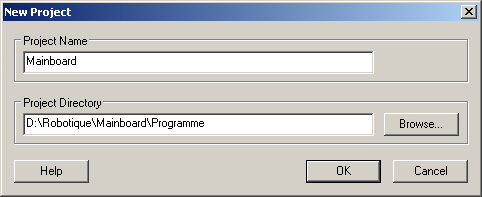
\includegraphics[scale=0.75]{Images/Fenetre_nouveau_projet.png}
			\caption{Fenêtre \og{}nouveau projet\fg{} dans MPLAB \ac{IDE}
				\label{Fenetre_nouveau_projet}}
		\end{figure}
	\item Ouvrir le menu \og{}Project\fg{} $\rightarrow$ \og{}Build Options\fg{} $\rightarrow$ \og{}Projet\fg{} ;
	\item Dans l'onglet \og{}General\fg{}, renseignez les champs suivant, comme illustré figure \ref{Build_Options_General} :
		\begin{itemize}
			\item Include Search Path, \$(INCDIR)
			\item Library Search Path, \$(LIBDIR)
			\item Linker-Script Search Path, \$(LKRDIR)
		\end{itemize}

Astuce : pour chaque champ, cliquez sur \og{}Browse\fg{}, puis appuyez sur \Enter{}, cela le renseignera avec la valeur par défaut que nous avons configurées auparavant dans \og{}Language Tool Locations\fg{} ;
		\begin{figure}[H]
			\centering
			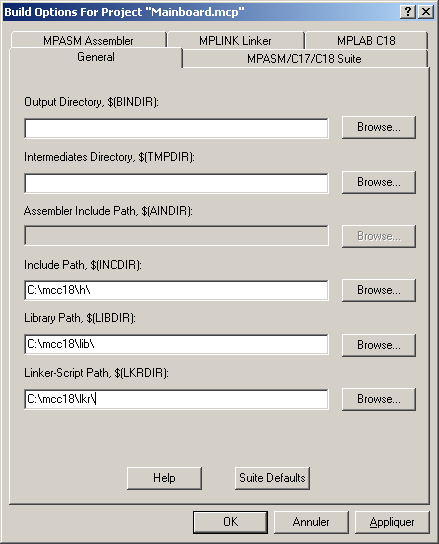
\includegraphics[scale=0.75]{Images/Build_Options_General.png}
			\caption{Fenêtre \og{}Build Options\fg{} du projet
				\label{Build_Options_General}}
		\end{figure}
	\item Dans l'onglet \og{}MPLINK Linker\fg{} de la même fenêtre, vous pouvez si vous le souhaitez cocher la case \og{}Generate map file\fg{}. Ainsi, le compilateur génèrera un fichier .map contenant toutes les variables utilisées dans le programme et leur adresse physique dans le PIC, ce qui peut avoir son utilité ;
	\item Il nous faut ensuite ajouter le fichier de script du linker qui correspond au PIC pour lequel on écrira le programme (18f452.lkr dans notre cas), en cliquant du bouton droit de la souris sur l'intitulé \og{}Linker Scripts\fg{} du volet contenant les fichiers du projet, comme illustré figure \ref{Ajout_script_linker}. Les fichiers .lkr se trouvent dans le sous-répertoire {\ttfamily lkr} du répertoire d'installation de MPLAB C18 (par exemple, {\ttfamily C:$\backslash$mcc18$\backslash$lkr}) ;
		\begin{figure}[H]
			\centering
			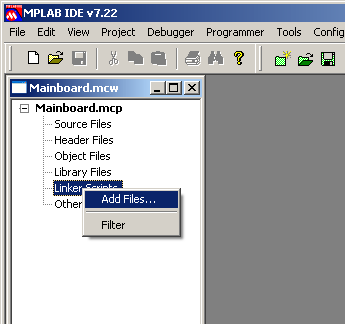
\includegraphics[scale=0.75]{Images/Ajout_script_linker.png}
			\caption{Ajout du script du linker dans MPLAB \ac{IDE}
				\label{Ajout_script_linker}}
		\end{figure}
	\item Créer un fichier source via le menu \og{}File\fg{} $\rightarrow$ \og{}New\fg{} et enregistrez-le dans le répertoire du projet avec l'extension \og{}.c\fg{} (à l'aide du menu \og{}File\fg{} $\rightarrow$ \og{}Save As...\fg{}). Ajoutez ensuite ce fichier à l'intitulé \og{}Source Files\fg{} du volet contenant les fichiers du projet, en procédant de la même manière que pour le fichier de script du linker ;
	\item Configurer le projet pour qu'il utilise le langage C18 : ouvrez le menu \og{}Project\fg{} $\rightarrow$ \og{}Select Language Toolsuite\fg{} et choisissez \og{}Microchip C18 Toolsuite\fg{} comme \og{}Active Toolsuite\fg{} dans la boite de dialogue qui apparaît alors ;
	\item Préciser le modèle de PIC du projet, dans le menu \og{}Configure\fg{} $\rightarrow$ \og{}Select Device...\fg{}, sélectionnez le PIC que vous allez utiliser (nous utiliserons par la suite le PIC18F452).
\end{enumerate}

Vous avez désormais en principe correctement configuré votre projet. Il ne reste plus qu'à écrire le programme. Pour le compiler, sélectionnez \og{}Project\fg{} $\rightarrow$ \og{}Make\fg{} ou \og{}Project\fg{} $\rightarrow$ \og{}Build all\fg{}. Un fichier hexadécimal .hex est alors créé dans le répertoire du projet (ou dans le répertoire Output si vous l'avez spécifié). C'est ce fichier qu'il faudra par la suite transférer sur le PIC.

\subsubsection{Transfert du programme sur le PIC}

Pour transférer le programme sur le PIC, nous allons utiliser ICPROG. La procédure pour programmer le PIC18F452 décrire ci-après suppose que les options de configuration sont au départ celles par défaut. Il vous est toujours possible de réinitialiser la configuration par défaut dans le menu \og{}Settings\fg{} $\rightarrow$ \og{}Clear Settings\fg{}.

\paragraph{Installation de ICPROG sous Windows NT/2000/XP}

Si vous êtes sous Windows NT/2000/XP, en plus d'avoir les droits administrateur, il est nécessaire d'installer un driver spécifique pour que le programme fonctionne. Pour cela, il vous faut télécharger le fichier icprog.sys correspondant à votre version d'ICPROG, sur le site de l'auteur, et le placer dans le même répertoire que le programme.

\begin{figure}[H]
	\centering
	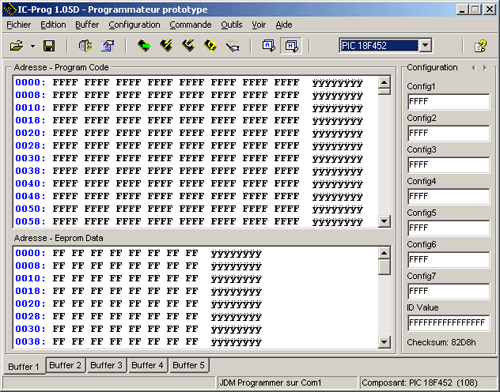
\includegraphics[scale=0.75]{Images/ICPROG.png}
	\caption{Le programme ICPROG (configuré pour être en langue française)
		\label{ICPROG}}
\end{figure}

Vous devez ensuite configurer ICPROG pour utiliser ce driver. Pour cela, allez dans le menu \og{}Settings\fg{} $\rightarrow$ \og{}Options\fg{}, puis dans l'onglet \og{}Misc\fg{}. Cochez alors la case \og{}Enable NT/2000/XP Driver\fg{} (voir figure \ref{ICPROG_Enable_NT_Driver}). Relancer le programme, qui vous demandera alors si vous désirez installer le driver, auquel vous répondrez donc oui.

\begin{figure}[H]
	\centering
	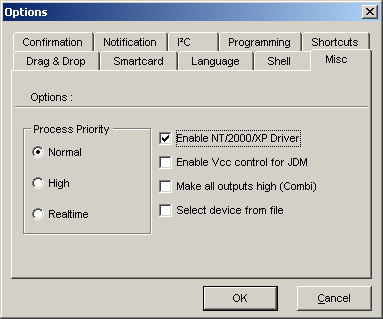
\includegraphics[scale=0.75]{Images/ICPROG_Enable_NT_Driver.png}
	\caption{Activer le driver Windows NT avec ICPROG
		\label{ICPROG_Enable_NT_Driver}}
\end{figure}

Vous pouvez en profiter pour éventuellement mettre ICPROG en français, dans l'onglet \og{}Language\fg{} de la même fenêtre et nous supposerons pour la suite qu'ICPROG est configuré en français.

Allez ensuite dans le menu \og{}Configuration\fg{} $\rightarrow$ \og{}Hardware\fg{} et sélectionnez \og{}Windows API\fg{} dans l'encadré intitulé \og{}Interface\fg{} (voir figure \ref{ICPROG_Hardware_Settings}). C'est indispensable pour que le programme utilise le driver que nous venons d'installer.

\begin{figure}[H]
	\centering
	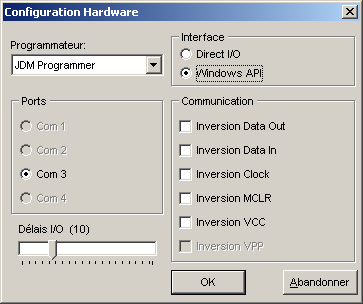
\includegraphics[scale=0.75]{Images/ICPROG_Hardware_Settings.png}
	\caption{Fenêtre de configuration Hardware dans ICPROG
		\label{ICPROG_Hardware_Settings}}
\end{figure}

\paragraph{Choix du programmateur}

Vous trouverez un schéma de programmateur série de type JDM figure \ref{Programmateur_JDM}. Ce programmateur a l'avantage d'être très simple et il permet de programmation de PIC au format DIP18 et au format PLCC44 (notamment pour le PIC18F452, auquel nous nous intéresserons plus particulièrement).

\begin{figure}[H]
	\centering
	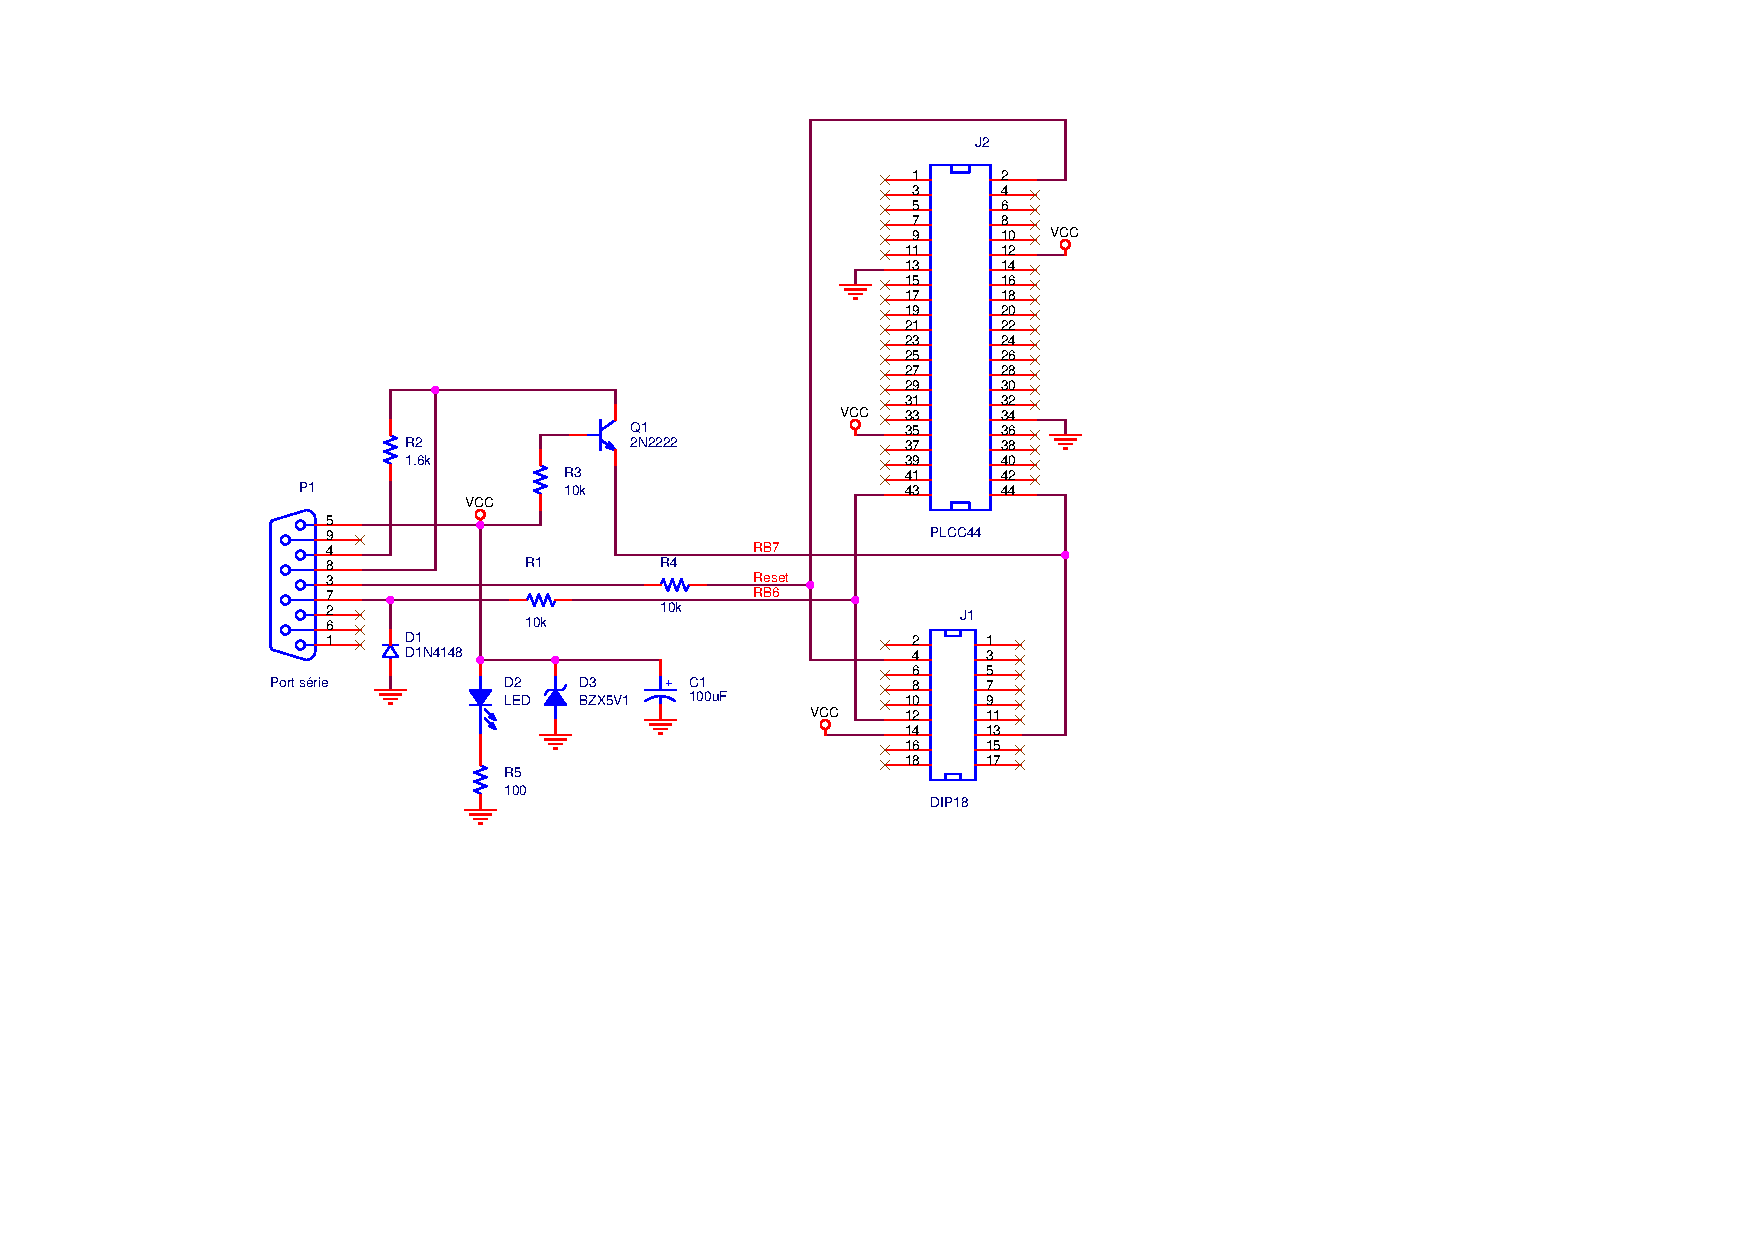
\includegraphics[scale=1.00]{Images/Programmateur_JDM}
	\caption{Programmateur de PIC sur port série, type JDM
		\label{Programmateur_JDM}}
\end{figure}

\paragraph{Transfert du programme}

Avant de transférer le programme, il vous faut correctement configurer ICPROG pour le programmateur et le PIC que vous utilisez. Cela se fait dans la fenêtre de configuration Hardware d'ICPROG. Pour le programmateur présenté précédemment, la configuration est celle par défaut, illustrée figure \ref{ICPROG_Hardware_Settings}. Pour le PIC, il vous suffit de sélectionner le bon modèle dans le menu déroulant de la fenêtre principale, en surbrillance, en haut à droite figure \ref{ICPROG}.

Ensuite, vous n'avez plus qu'à charger le fichier .hex généré par le compilateur (\og{}Fichier\fg{} $\rightarrow$ \og{}Ouvrir Fichier...\fg{}) et lancer la programmation (\og{}Commande\fg{} $\rightarrow$ \og{}Tout Programmer\fg{}, ou \keystroke{F5}), après s'être assuré que le PIC est correctement en place sur le programmateur (attention au sens) et que celui-ci est bien connecté au port série du PC. Vérifiez que le bon port COM est sélectionné dans la fenêtre figure \ref{ICPROG_Hardware_Settings}.

Il ne doit y avoir qu'une seule fenêtre d'ICPROG ouverte et aucun autre programme ne doit accéder au port COM sur lequel est connecté le programmateur durant la lecture ou la programmation du PIC.

Afin de contrôler le bon déroulement de la programmation et de gagner du temps, vous pouvez activer l'option \og{}Vérifier pendant la programmation\fg{}, de l'onglet \og{}Programmation\fg{}, du menu \og{}Configuration\fg{} $\rightarrow$ \og{}Options\fg{}. Ainsi s'il y a un problème, vous n'aurez pas à attendre la fin de la programmation pour le savoir.

\subsection{Caractéristiques du PIC18F452}

\subsubsection{Le composant}

\begin{figure}[H]
	\centering
	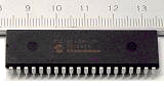
\includegraphics[scale=0.75]{Images/PIC18F452_DIP40.png}
	\caption{PIC18F452-I/P (format DIP, 40 broches)
		\label{PIC18F452_DIP40}}
\end{figure}

\begin{figure}[H]
	\centering
	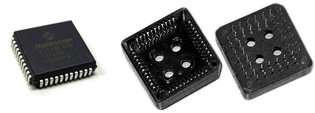
\includegraphics[scale=0.75]{Images/PIC18F452_PLCC44.png}
	\caption{PIC18F452-I/L + support (format PLCC, 44 broches, dont 4 broches non connectés)
		\label{PIC18F452_PLCC44}}
\end{figure}

Le PIC18F452 au format PLCC44 requiert un support spécial, représenté figure \ref{PIC18F452_PLCC44}. Noter que pour retirer le PIC du support proprement et sans risque, il existe une pince spécialement prévu à cet effet, représentée figure \ref{Pince_PLCC44} (pour extraire le composant du support, il faut presser la pince et ne jamais la tirer).

\begin{figure}[H]
	\centering
	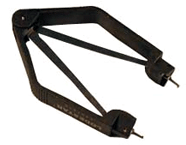
\includegraphics[scale=0.75]{Images/Pince_PLCC44.png}
	\caption{Pince PLCC44
		\label{Pince_PLCC44}}
\end{figure}

\subsubsection{L'horloge (CLOCK)}

L'horloge synchronise toutes les actions du processeur (système synchrone).\\
Il y a 8 types d'oscillateurs possibles et 3 schémas d'horloge :

\begin{itemize}
	\item Résonateur à quartz ou à céramique ;
	\item Oscillateur RC - Résistance-Capacité ;
	\item Horloge externe.
\end{itemize}

$\Rightarrow$ Voir datasheet §2 \cite{PIC18FXX2}.

\subsubsection{L'initialisation (RESET)}

Le RESET force l'état initial du circuit.\\
Il y a 6 sources de RESET distinctes, le RESET de base étant le \og{}Power-on Reset\fg{} (POR), qui initialise le circuit à la mise sous tension.

$\Rightarrow$ Voir datasheet §3 \cite{PIC18FXX2}.

\subsubsection{La mémoire}

Il y a trois types de mémoire :

\begin{itemize}
	\item 32 Ko de mémoire programme, ou mémoire FLASH : contient le programme ;
	\item 1536 octets de mémoire vive, ou RAM (Random Access Memory) : contient les données en cours de traitement ;
	\item 256 octets d'EEPROM : mémoire rapide de stockage de données.
\end{itemize}

$\Rightarrow$ Voir datasheet §4, §5 et §6 \cite{PIC18FXX2}.

\subsubsection{Les entrées/sorties}

\begin{itemize}
	\item 34 entrées/sorties réparties sur 5 ports ;
	\item 8 canaux de conversion A/N (analogique/numérique) ;
	\item 2 modules CCP : Capture/Compare/PWM (PWM - Pulse With Modulation = MLI - Modulation de Largeur d'Impulsion) ;
	\item 18 sources d'interruption.
\end{itemize}

\begin{figure}[H]
	\centering
	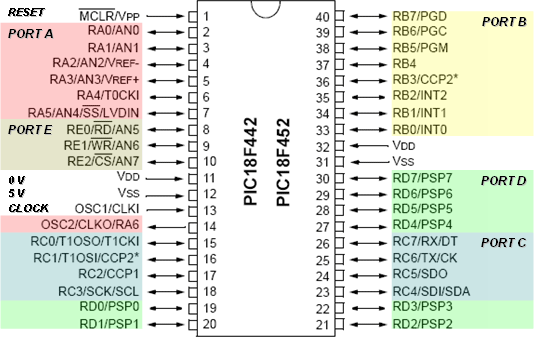
\includegraphics[scale=0.75]{Images/Pins_PIC18F452.png}
	\caption{Les PINs du PIC18F452 (pour le format DIP)
		\label{Pins_PIC18F452}}
\end{figure}

$\Rightarrow$ Voir datasheet §9, §14 \cite{PIC18FXX2}.

\subsubsection{Les timers}

Il y a 4 timers disponibles. Un timer a fonction de compteur programmable, le comptage pouvant se faire sur 8 ou 16 bits. Il y a deux sources de comptage :

\begin{itemize}
	\item Horloge du PIC ;
	\item Front montant/descendant sur l'entrée T0CKI ou T1CKI.
\end{itemize}

Les interruptions sont générées sur les overflow.

$\Rightarrow$ Voir datasheet §10 à §13 \cite{PIC18FXX2}.

\subsection{Un montage de base}

\begin{figure}[H]
	\centering
	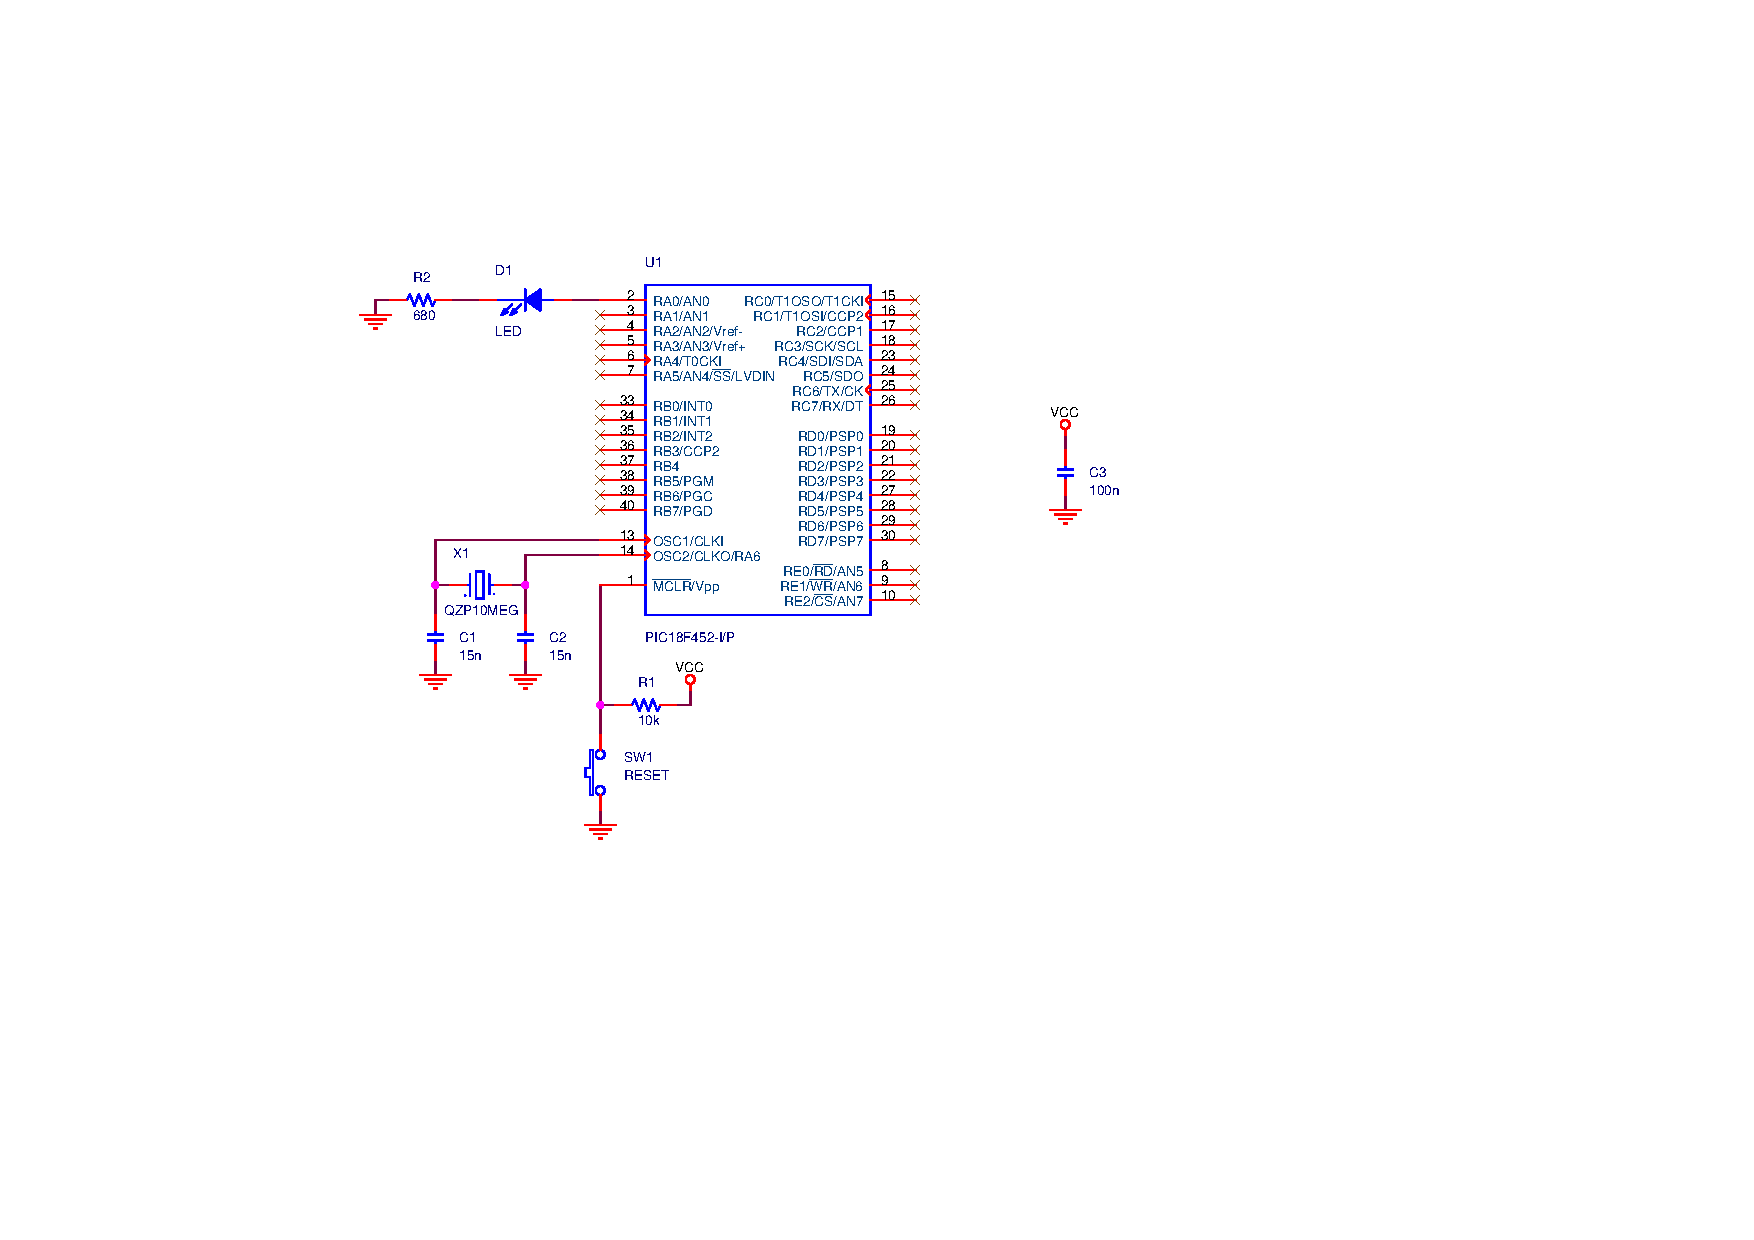
\includegraphics[scale=1.00]{Images/Montage_base_PIC18F452}
	\caption{Montage de base du PIC18F452
		\label{Montage_base_PIC18F452}}
\end{figure}

Vous noterez la présence d'une capacité de découplage au niveau de l'alimentation (les broches d'alimentation du PIC ne sont pas représentées sur ce schéma, mais elles existent bien et le logiciel sait qu'elles sont reliées sur VCC et GND). Cette capacité devra être monté en pratique le plus proche possible du PIC.\\
Une résistance de tirage est utilisée sur le RESET (entrée $\overline{MCLR}$ du PIC). Il s'agit là de la circuiterie de reset la plus basique qu'il soit possible de faire.\\
Une résistance de limitation de courant est présente pour la \ac{LED}.\\
Enfin, le quartz et les deux condensateurs assurent l'horloge du PIC.

\subsection{La programmation}

\subsubsection{Faire clignoter une LED}

Nous considérons le montage de la figure \ref{Montage_base_PIC18F452}. Le programme suivant permet de faire clignoter la \ac{LED} D1. C'est l'un des programmes les plus simples qui soit et qui est très pratique pour tester le bon fonctionnement des montages, qui devraient toujours avoir une \ac{LED} témoin permettant d'afficher l'état du PIC.

\begin{lstlisting}[caption=Programme faisant clignoter une \ac{LED}, label=Programme_faisant_clignoter_une_LED, language=c]
#include <p18f452.h>	// déclarations pour le PIC18F452
#include <delays.h>		// fonctions de délais

// Configuration
#pragma config OSC = HSPLL	// oscillateur HS, avec PLL (fréquence multipliée par 4)
#pragma config PWRT = ON		// power up timer (activé)
#pragma config WDT = OFF		// watchdog timer (desactivé)
#pragma config BOR = ON			// brown out reset (activé)
#pragma config BORV = 42		// brown out voltage (4.2V)
#pragma config LVP = ON			// low voltage ICSP (activé)

void main(void) {
	// On configure le pin 0 du port A en sortie
	TRISAbits.TRISA0 = 0;

	while(1) {
		// On allume la LED en mettant le pin 0 à l'état haut
		PORTAbits.RA0 = 1;
		// On attends environ 0,25s à 40Mhz
		Delay10KTCYx(0);

		// On éteint la LED en mettant le pin 0 à l'état bas
		PORTAbits.RA0 = 0;
		// On attends environ 0,25s à 40Mhz
		Delay10KTCYx(0);
	}
}
\end{lstlisting}

\paragraph{Algorithme}

L'algorithme, très simple, est présenté figure \ref{Algorithme_clignoter_LED}.

\begin{figure}[H]
	\centering
	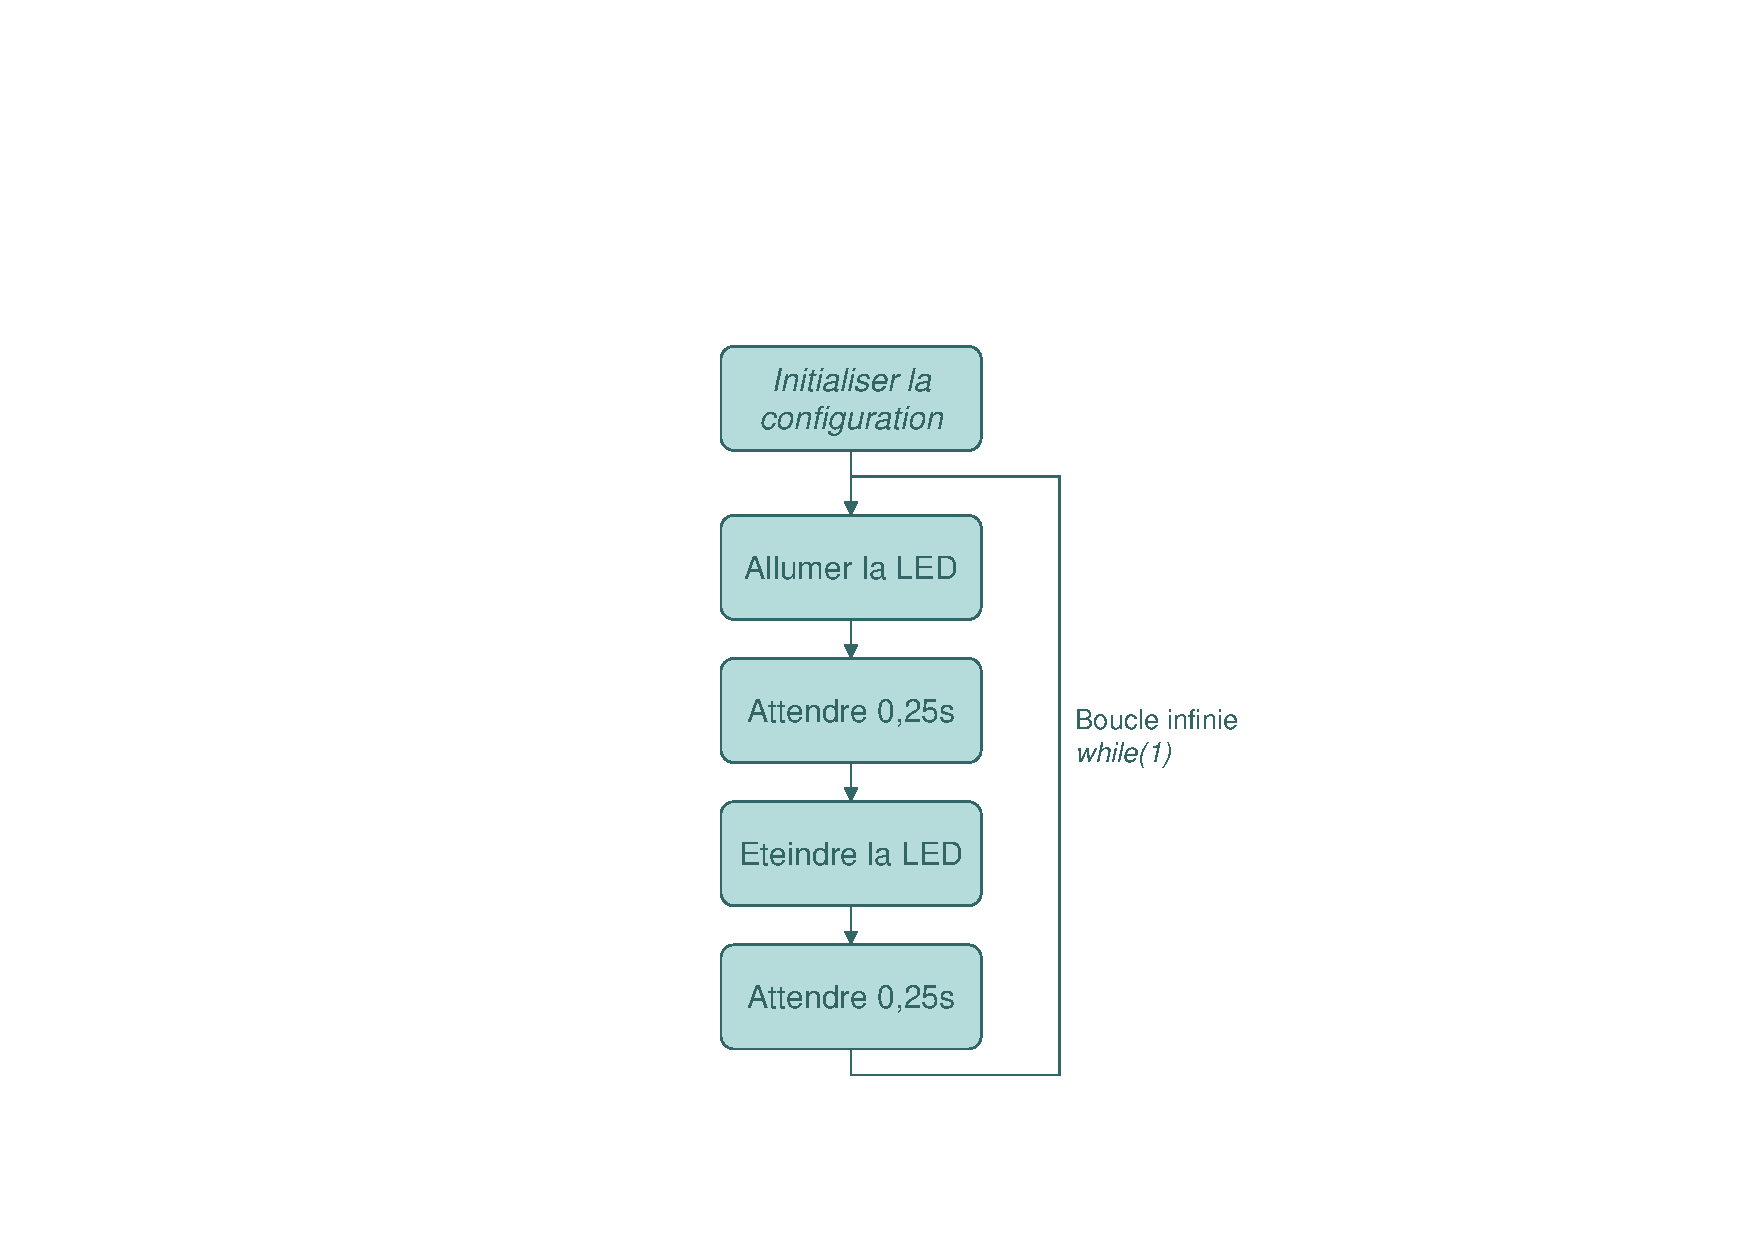
\includegraphics[scale=0.60]{Images/Algorithme_clignoter_LED}
	\caption{Algorithme du programme faisant clignoter une \ac{LED}
		\label{Algorithme_clignoter_LED}}
\end{figure}

\paragraph{Inclusion des librairies}

Pour ce programme, deux librairies sont nécessaires :

\begin{itemize}
	\item \og{}p18f452.h\fg{} : déclarations des constantes relatives au PIC18F452, requis pour PORTAbits.RA0.\\
	$\Rightarrow$ Voir les fichiers *.h du répertoire \og{}h\fg{} de MPLAB C18.
	\item \og{}delays.h\fg{} : fonctions de délais, requis pour la fonction Delay10KTCYx().\\
	$\Rightarrow$ Voir MPLAB C18 C Compiler Libraries §4.5.
\end{itemize}

\subsubsection{Les interruptions}

Un PIC n'est pas multitâches (comme tout processeur d'ailleurs, puisque le multitâche est une couche logiciel), cela signifie qu'un seul code peut être exécuté à la fois. Les interruptions permettent au processeur d'exécuter une code qui n'est pas dans la boucle principale du programme, en réponse à un évènement, qui est donc appelé une interruption, quelque soit le code entrain d'être exécuté.

\paragraph{Illustration du problème}

On veut exécuter un calcul prenant 1s tout en faisant clignoter la \ac{LED}. Problème : durant le calcul, la \ac{LED} ne clignote pas !

\begin{figure}[H]
	\centering
	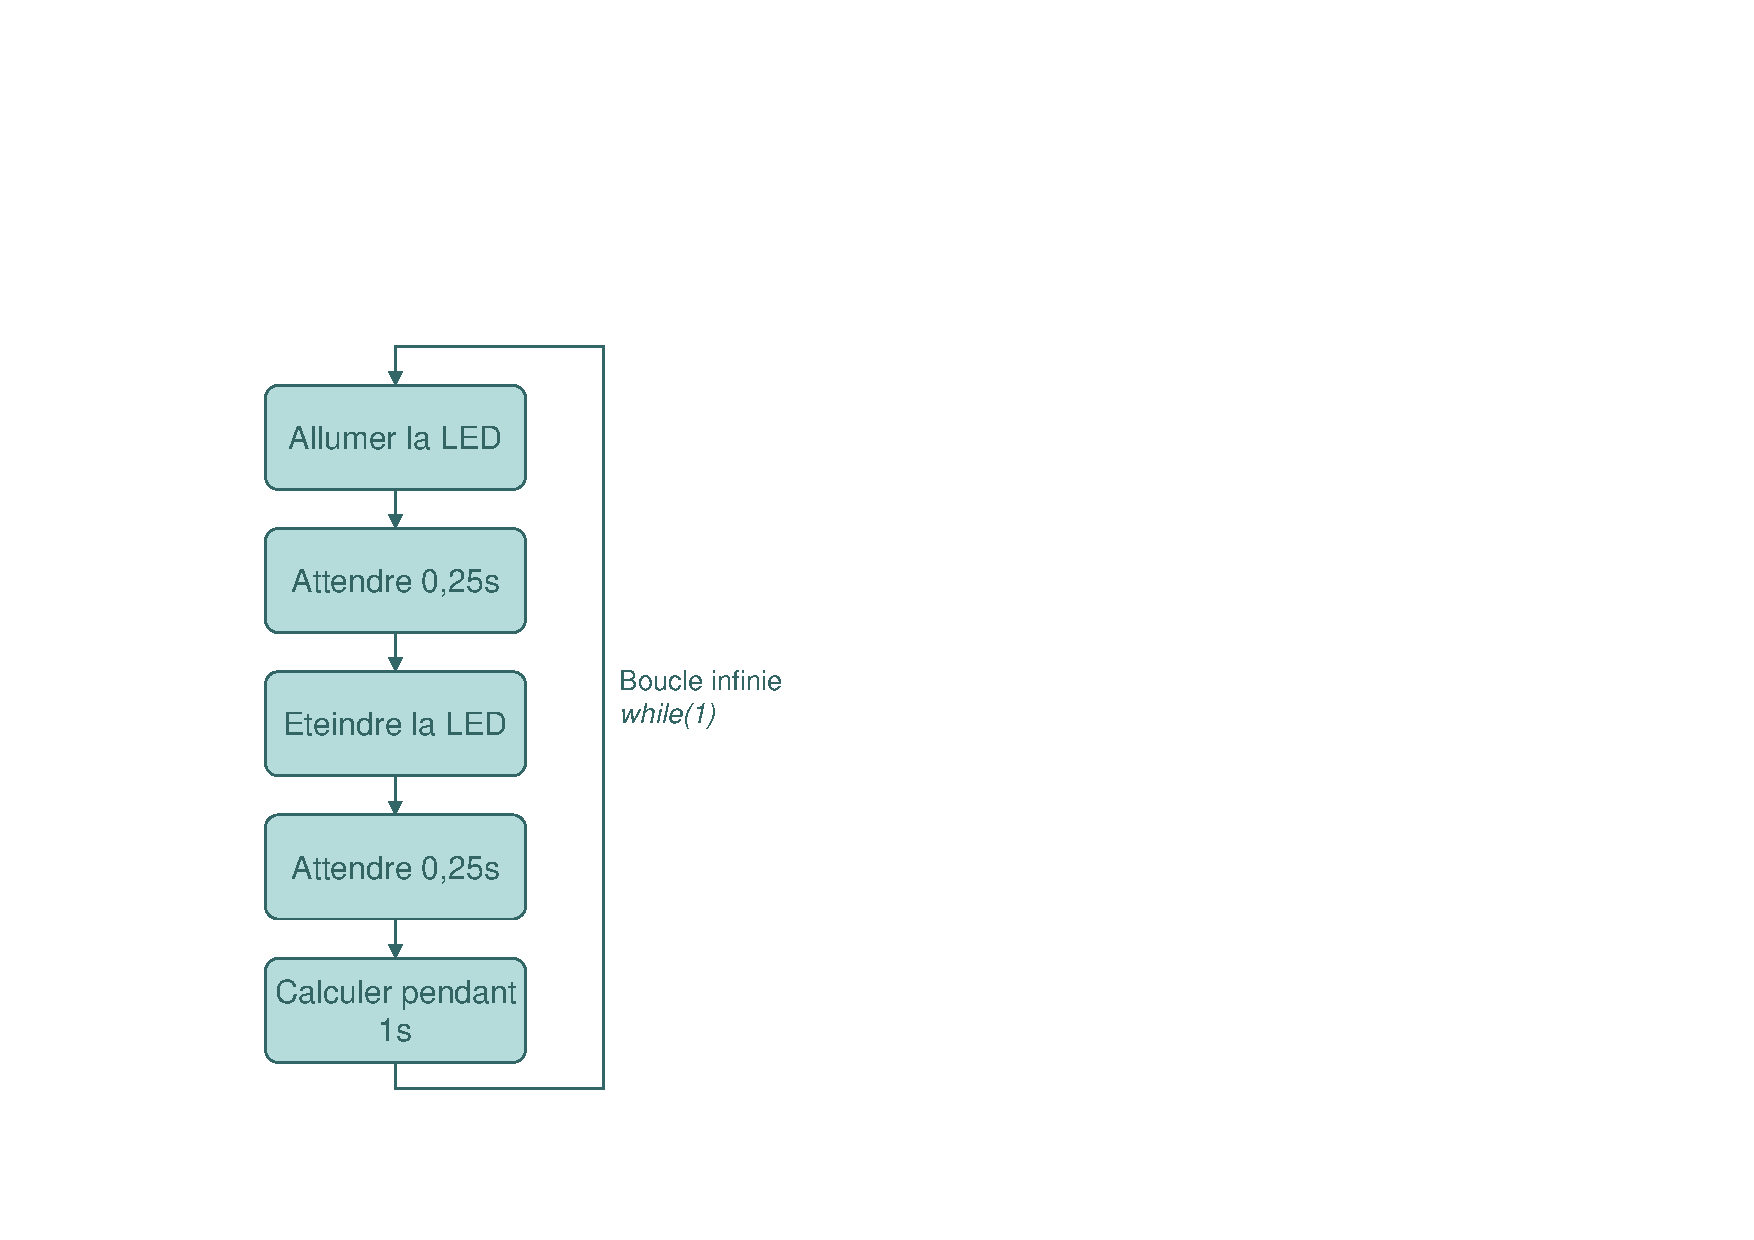
\includegraphics[scale=0.60]{Images/Interruptions_probleme}
	\caption{Algorithme sans interruption
		\label{Interruptions_probleme}}
\end{figure}

\paragraph{L'idée}

Introduction d'une interruption, qui survient lors d'un évènement (configurable) :

\begin{itemize}
	\item Overflow d'un timer ;
	\item Sur front montant/descendant d'une entrée INT0, INT1 ou INT2 ;
	\item Changement d'une entrée du port B ;
	\item ... .
\end{itemize}

$\Rightarrow$ Voir datasheet §8 \cite{PIC18FXX2}.

\begin{figure}[H]
	\centering
	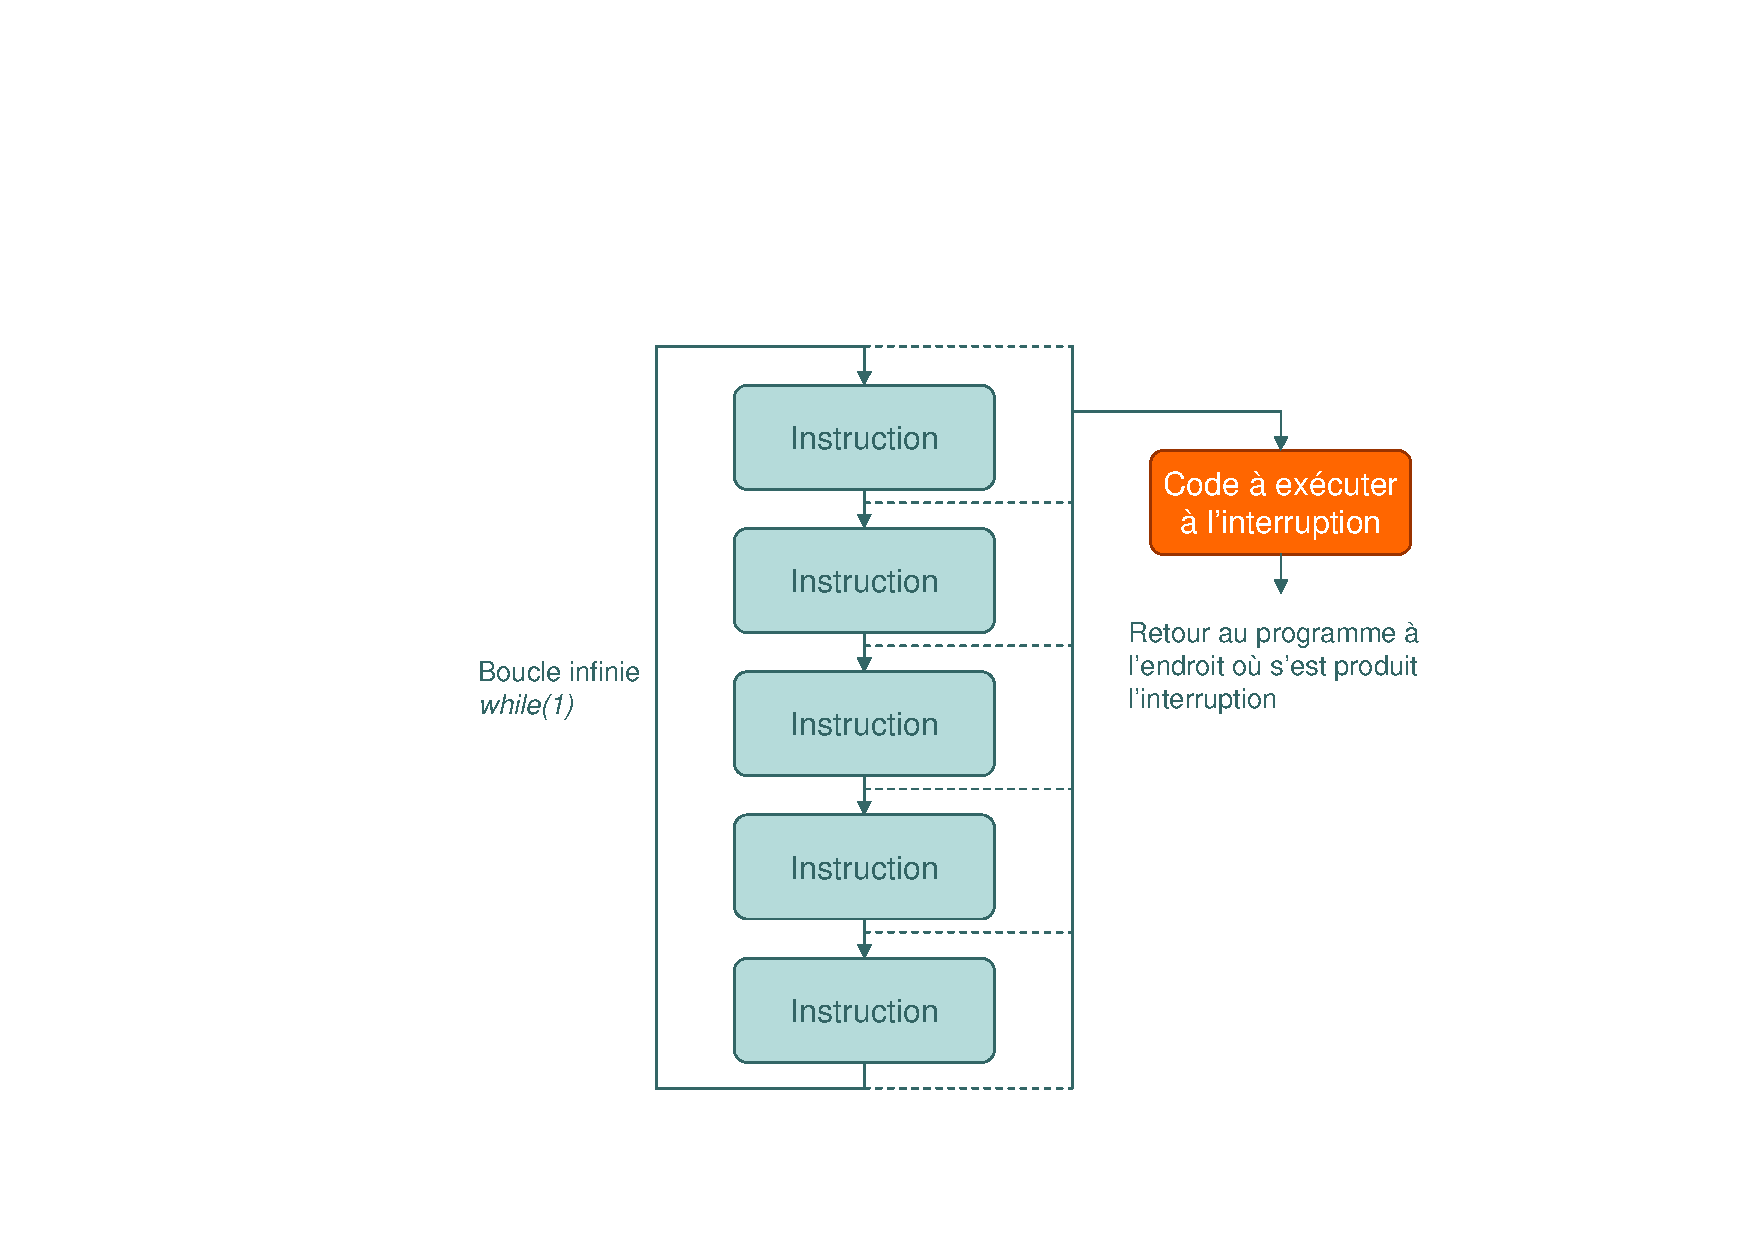
\includegraphics[scale=0.60]{Images/Interruptions_idee}
	\caption{Algorithme avec interruption
		\label{Interruptions_idee}}
\end{figure}

Retour sur l'exemple de la \ac{LED} : la solution est d'effectuer le calcul de 1s dans la boucle infinie et de générer une interruption toutes les 0,25s pour allumer ou éteindre la \ac{LED}. Cette interruption sera générée par un timer par exemple.

\paragraph{Les priorités}

Introduction de 2 niveaux de priorité, haute et basse. Une interruption de priorité basse peut elle-même être interrompue par une interruption de priorité haute.

\begin{figure}[H]
	\centering
	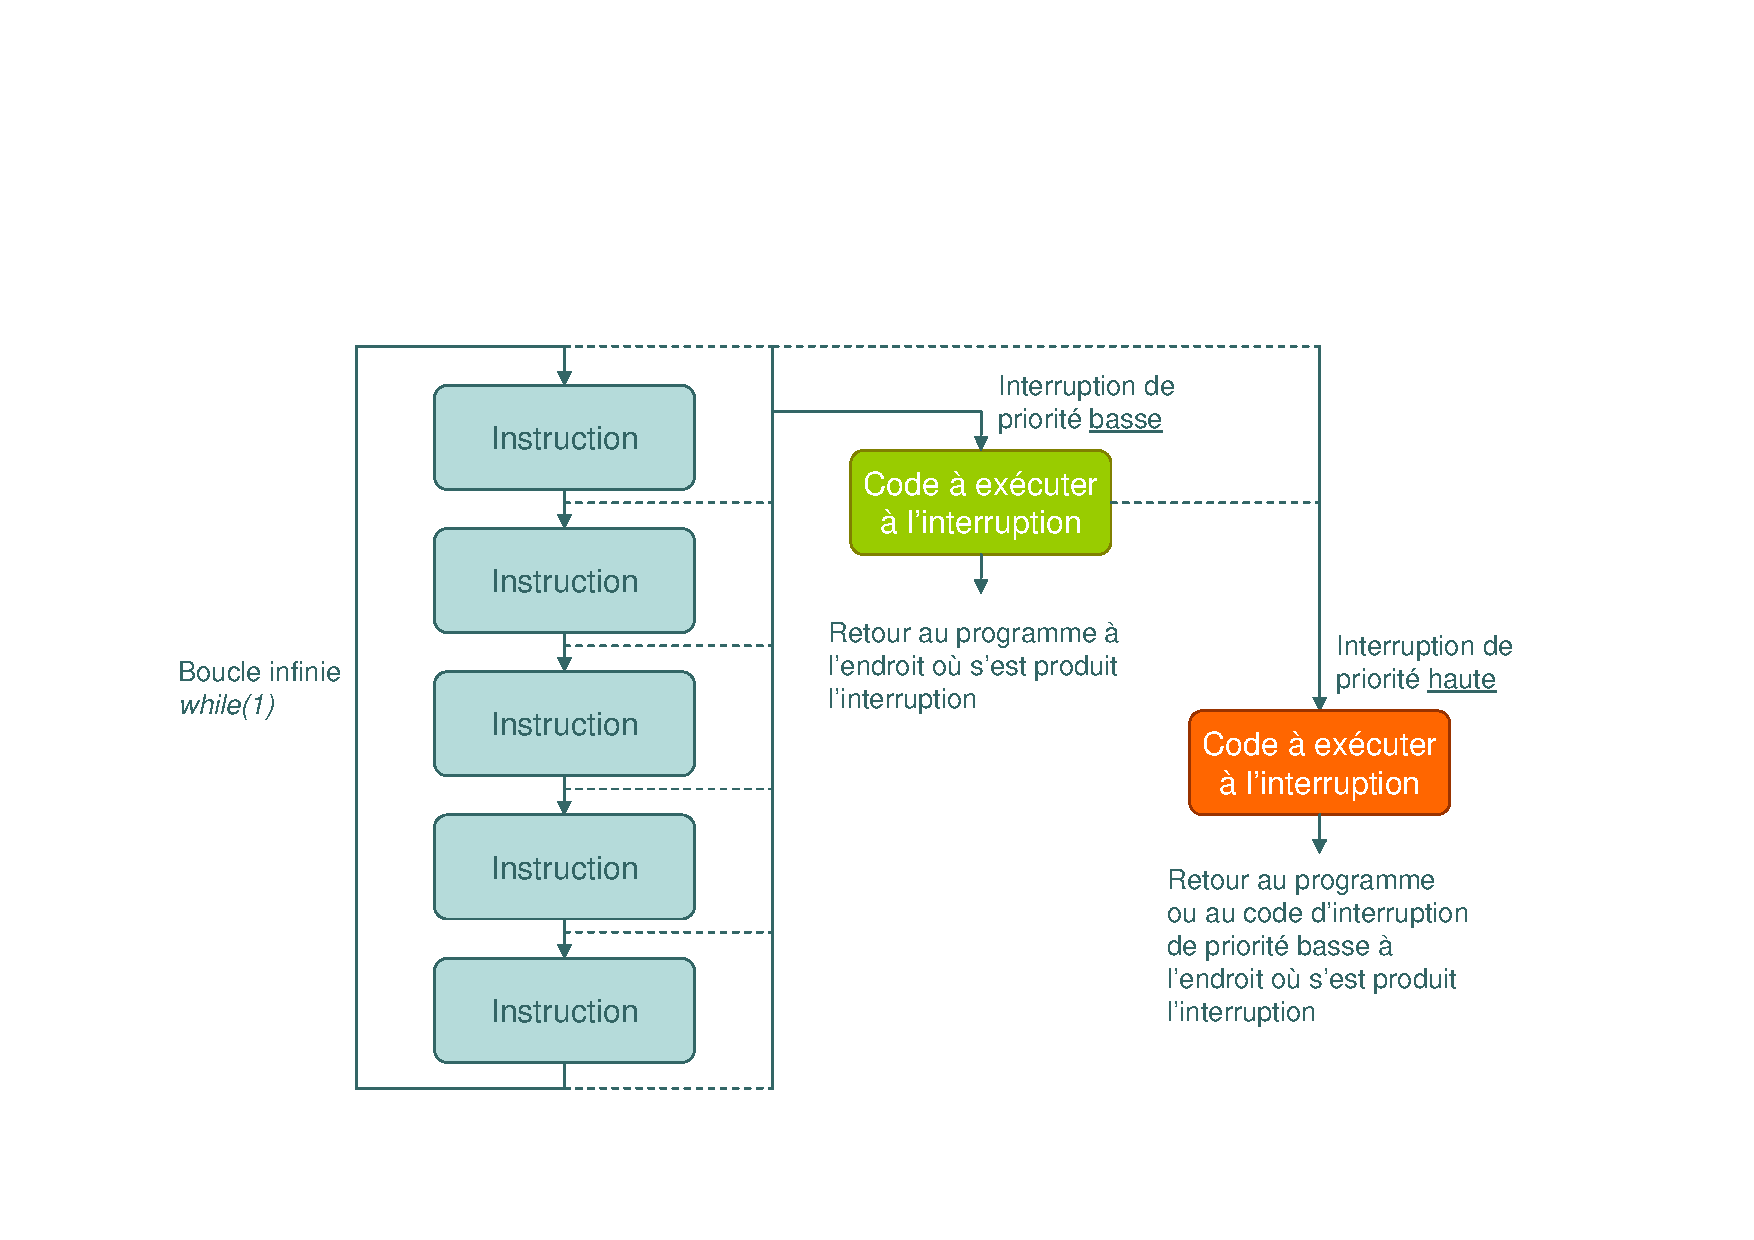
\includegraphics[scale=0.60]{Images/Interruptions_priorites}
	\caption{Les priorités dans les interruptions
		\label{Interruptions_priorites}}
\end{figure}

\subsubsection{Faire clignoter une LED sur interruption}

Nous considérons à nouveau le montage de la figure \ref{Montage_base_PIC18F452}. Le programme suivant permet de faire clignoter la \ac{LED} D1, cette fois-ci en utilisant les interruptions, ce qui permettra d'exécuter d'autres instructions dans la boucle principale au lieu d'attendre à chaque fois 0,25s sans rien faire.

\begin{lstlisting}[caption=Programme faisant clignoter une \ac{LED} sur interruption, label=Programme_faisant_clignoter_une_LED_sur_interruption, language=c]
#include <p18f452.h>	// déclarations pour le PIC18F452
#include <timers.h>		// fonctions pour les timers

// Configuration
#pragma config OSC = HSPLL	// oscillateur HS, avec PLL (fréquence interne multipliée par 4)
#pragma config PWRT = ON		// power up timer (activé)
#pragma config WDT = OFF		// watchdog timer (désactivé)
#pragma config BOR = ON			// brown out reset (activé)
#pragma config BORV = 42		// brown out voltage (4.2V)
#pragma config LVP = ON			// low voltage ICSP (activé)

// Prototype de la fonction interruption
void highISR(void); 

// Lors d'une interruption (de priorité haute ici)
#pragma code highVector=0x008
void interruptAtHighVector(void) {
	// On doit exécuter le code de la fonction highISR()
	_asm GOTO highISR _endasm
}
#pragma code // Retour à la zone de code

volatile short ledCount = 0;	// temporisation pour allumage de la LED toutes les 0,25s
volatile char ledStatu = 0;		// stocke l'état de la LED

#pragma interrupt highISR
void highISR(void) {
	unsigned char sProdL;
	unsigned char sProdH;

	// Sauvegarde du contenu des registres de calcul
	sProdL = PRODL;
	sProdH = PRODH;

	// C'est le Timer1 qui a levé l'interruption
	if (PIR1bits.TMR1IF) {
		WriteTimer1(64536); // 2^16 - 1000 : la prochaine interruption a lieu dans 1000 cycles = 100us

		ledCount++;

		if (ledCount >= 2500) {
			ledCount = 0;
			ledStatu = !ledStatu;
			PORTAbits.RA0 = ledStatu;
		}

		// On réautorise l'interruption
		PIR1bits.TMR1IF = 0;
	}

	// Restauration des registres de calcul
	PRODL = sProdL;
	PRODH = sProdH;
}

void main(void) {
	// On configure le pin 0 du port A en sortie
	TRISAbits.TRISA0 = 0;

	// On autorise toutes les interruptions
	INTCONbits.GIE = 1;
	INTCONbits.PEIE = 1;

	// Configuration du timer1
	PIE1bits.TMR1IE = 1;	// autorise les interruption par dépassement du Timer (Timer overflow)
	OpenTimer1(TIMER_INT_ON		// active le timer1
		 & T1_16BIT_RW					// compte sur 16 bits
		 & T1_SOURCE_INT				// utilise l'horloge interne
		 & T1_PS_1_1						// incrémente le compteur à chaque cycle (1:1)
		 & T1_OSC1EN_OFF				// pas d'oscillateur sur le timer1
		 & T1_SYNC_EXT_OFF			// ne pas se synchroniser sur une horloge externe
	);
	WriteTimer1(64536); // 2^16 - 1000 : la prochaine interruption a lieu dans 1000 cycles = 100us

	while(1) {
		// Boucle principale, désormais vide !
	}
}
\end{lstlisting}

\newpage
\part{Conception et réalisation de cartes}

\section{Utilisation d'OrCAD Capture}

\subsection{Créer un nouveau projet}

Pour créer un nouveau projet sous Capture, il suffit d'aller dans le menu \og{}File\fg{} $\rightarrow$ \og{}New\fg{} $\rightarrow$ \og{}Project...\fg{}. Donnez alors un nom et un emplacement au projet et cochez l'option \og{}Analog or Mixed A/D\fg{}. Sélectionnez ensuite \og{}Create a blanc project\fg{}. Vous vous retrouvez alors avec une page vide, qui correspond à la première (et unique pour le moment) page de votre nouveau projet.

\subsection{Prise en main}

\subsubsection{Les nets}

Tout d'abord, il faut comprendre le principe de fonctionnement des connections dans Capture : chaque ensemble de broches reliées entre elles correspond à une net. Capture attribut à chaque net un nom par défaut, composé d'un \og{}N\fg{} suivit par un nombre unique. Les connexions sont symbolisées par des fils ou des bus, mais peuvent également ne pas être représentés. Ainsi, si vous donnez le même nom à deux fils, à priori non connectés entre eux, ils appartiendront en réalité à la même net et seront pas conséquent reliés implicitement.

\begin{figure}[H]
	\centering
	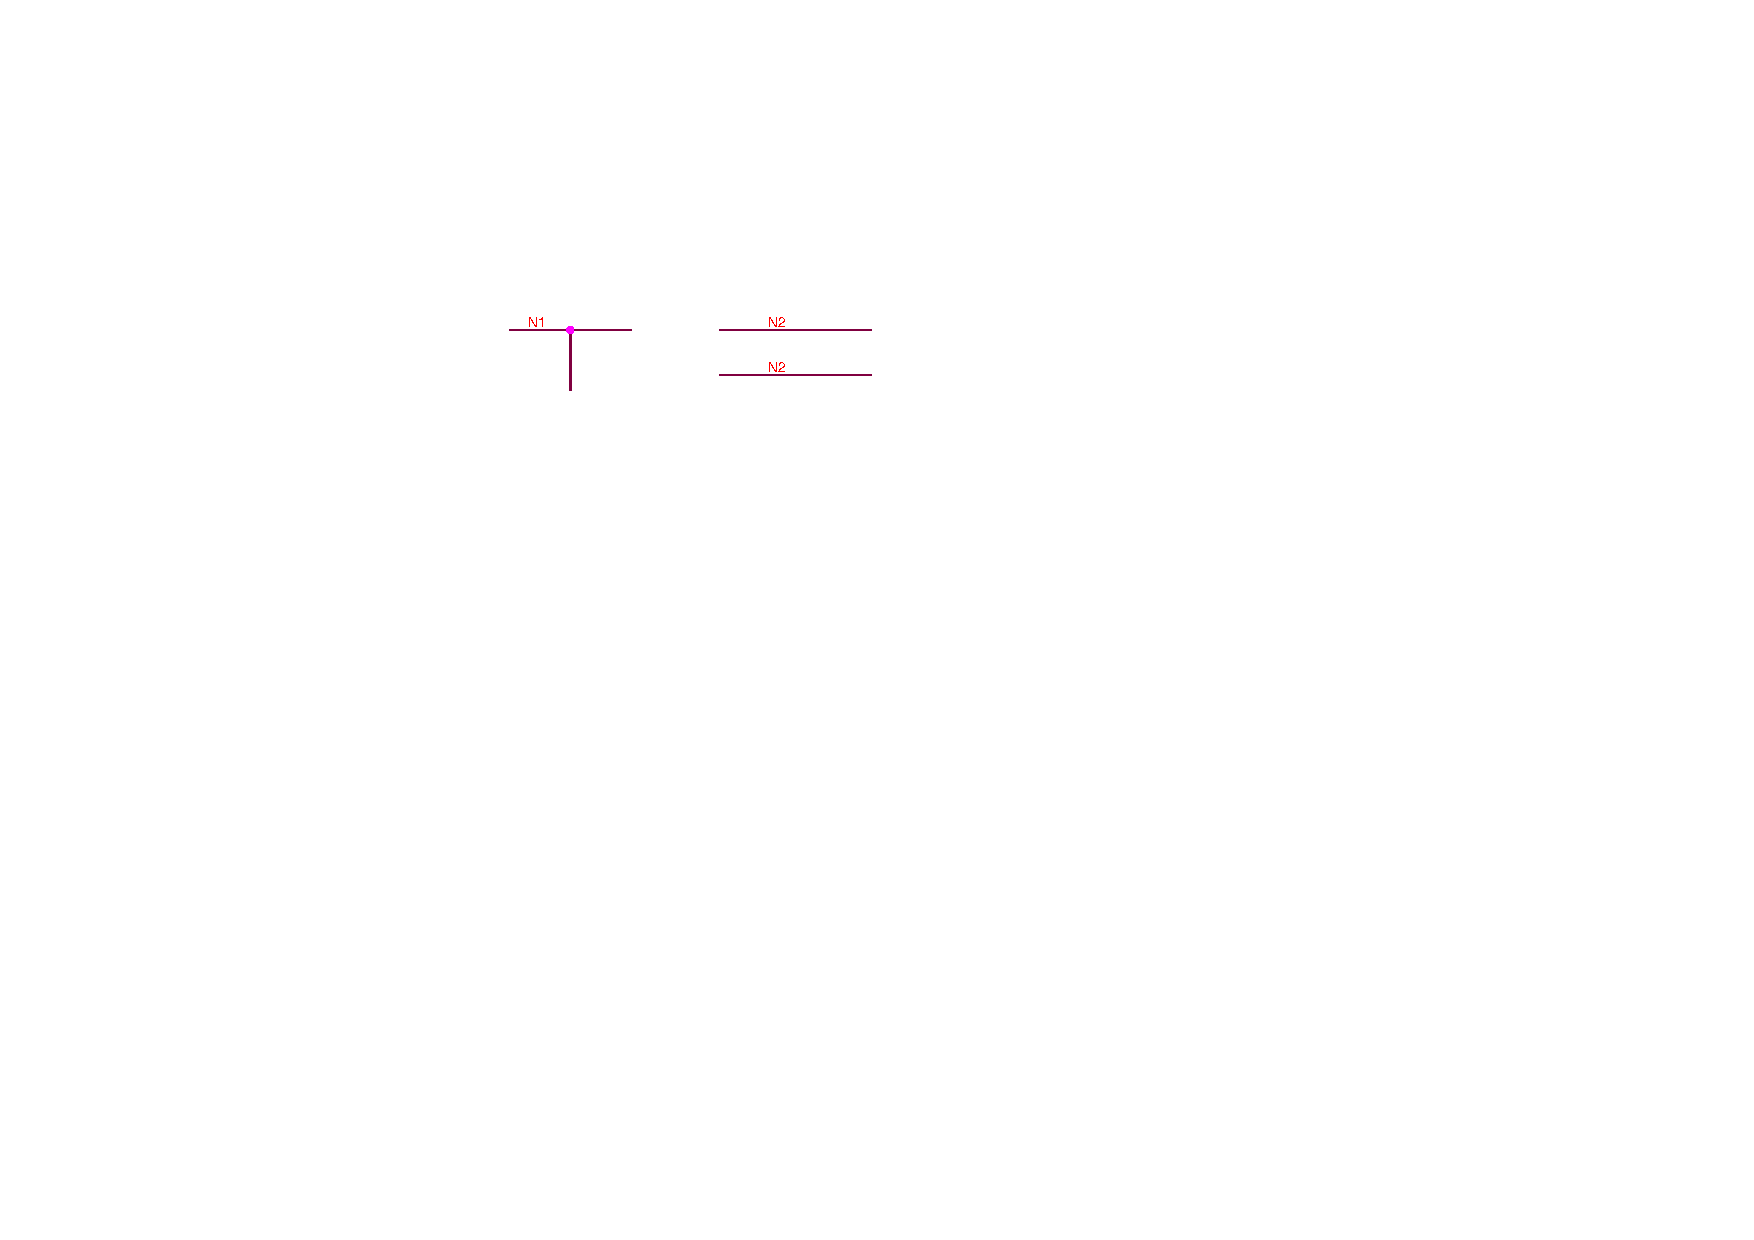
\includegraphics[scale=1.00]{Images/Les_nets_OrCAD}
	\caption{Les nets dans Capture
		\label{Les_nets_OrCAD}}
\end{figure}

Sur la figure \ref{Les_nets_OrCAD}, on a attribué un nom à chaque fil, qui vient remplacer le nom de net attribué par défaut par Capture. Une connexion entre deux fils est symbolisée par un point, comme pour la net N1. Les deux fils de droite ont le même nom de net, ils sont donc reliés entre eux, même si aucune connexion n'apparait sur le schéma.

Il est prudent de bien faire la distinction entre majuscules et minuscules pour les noms de net, et de ne pas nommer deux nets de la même manière en ne changeant que la case dans le nom.

Les noms et numéros des broches des composants n'ont pas de rapport avec le nom des nets donnés aux fils connectés dessus, excepté pour les broches d'alimentation (qui sont du type \og{}power\fg{}), dont le nom de net par défaut correspond au nom de la broche, tant que l'on a pas connecté de fil dessus, qui vienne changer le nom de la net.

\subsubsection{Les alimentations}

Dans la mesure où nous ne désirons pas simuler notre projet, il ne faut placer aucun générateur sur le schéma du circuit, en vue de l'exporter ensuite sous Layout afin de créer le \ac{PCB} de la carte. Il faut par contre évidemment prévoir les connecteurs d'alimentation.

En outre, il existe sous Capture plusieurs symboles pour l'alimentation et la masse. Le 0 V est généralement désigné par GND, tandis que le 5 V est désigné par VCC, en ce qui concerne les noms de nets. Cette convention doit absolument être respecté sous Capture, car de nombreux composants schématisés dans les librairies du programme alimenté en 5 V utilisent ces noms pour les broches d'alimentation et de masse, qui n'apparaissent pas toujours sur le schéma, mais qui appartiennent tout de même aux nets VCC et GND respectivement.

Si une autre tension d'alimentation doit intervenir, il faut donc la nommer autrement, par exemple \og{}VDD\fg{} (qui est généralement le nom de la broche d'alimentation des composants lorsque ceux-ci ne sont pas alimentés en 5 V) ou \og{}12V\fg{} et utiliser de préférence un autre symbole d'alimentation.

\begin{figure}[H]
	\centering
	\includegraphics[scale=1.00]{Images/Symboles_alim_OrCAD}
	\caption{Quelques symboles d'alimentation dans Capture
		\label{Symboles_alim_OrCAD}}
\end{figure}

Le nom de net correspond au nom du symbole pour les différents VCC et GND. Pour les symboles de masse, leur nom n'est simplement pas affiché (sauf pour le symbole nommé \og{}0\fg{}, le nom de la net étant alors \og{}0\fg{}). Le symbole de masse standard est celui représenté en bas à gauche de la figure \ref{Symboles_alim_OrCAD}, dont le nom est \og{}GND\fg{}.

\subsubsection{Les bus}

Les bus représentent des paquets de fils et permettent de simplifier les schémas électroniques et faciliter leur lecture. On peut voir un bus, représenté par un trait plus épais dans Capture, comme une gaine dans laquelle place plusieurs fils. Notez que l'on ne peut pas directement relier un fil au bus, pour cela, il faut placer une \og{}bus entry\fg{}, représenté par un bout de fil tourné de 45°. La figure \ref{Bus_OrCAD} illustre un bus schématisé sous Capture.

\begin{figure}[H]
	\centering
	\includegraphics[scale=1.00]{Images/Bus_OrCAD}
	\caption{Représentation d'un bus sous Capture
		\label{Bus_OrCAD}}
\end{figure}

Vous devez maintenant vous poser une question : comment savoir qu'à un certain fil entrant sur le bus correspond tel autre fil relié au bus ? Il faut pour cela utiliser des \og{}net alias\fg{}, et donner le même nom de net aux deux fils, comme cela a été fait figure \ref{Bus_OrCAD}. Connecter les fils à un bus n'est d'ailleurs qu'une mise en forme, puisque les deux fils sont reliés à partir du moment où ils ont le même nom de net.

En principe, il faut nommer les bus dans Capture, avec un nom de la forme \og{}busname[m:n]\fg{}, où m et n sont des entiers qui indiquent respectivement le premier et le dernier indice des nets connectés au bus (et le nom du bus ne doit pas se terminer par un chiffre). Par exemple, le bus \og{}bus[1:3]\fg{} contiendra les nets \og{}bus1\fg{}, \og{}bus2\fg{} et \og{}bus3\fg{}.

Il n'est donc pas possible, si l'on respecte scrupuleusement cette règle, de connecter des nets aux noms différents, hormis l'indice. En pratique, il n'est pas nécessaire de nommer les bus et l'on a pas à se soucier des noms des nets qui y sont connectés, si l'on se contente d'exporter la netlist de notre schéma sous Layout. Cela peut toutefois poser problème pour d'autres exports (un bus non nommé provoque d'ailleurs une erreur \ac{DRC} dans Capture) !

\subsubsection{Les principales librairies}

\begin{table}[H]
	\centering
	\begin{tabular}{|l|l|}\hline
			Librairie (.olb) & Composants\\\hline\hline
			{\ttfamily ANALOG} & \\
			 & \includegraphics[scale=1.00]{Images/OrCAD_analog_olb}\\\hline
			{\ttfamily DISCRETE} & \\
			 & \includegraphics[scale=1.00]{Images/OrCAD_discrete_olb}\\
			 & Diodes, transformateurs, relais...\\\hline
			{\ttfamily CONNECTOR} & \\
			 & \includegraphics[scale=1.00]{Images/OrCAD_connector_olb}\\
			 & Tous types de connecteurs\\\hline
			{\ttfamily ARITHMETIC} & \ac{CMOS} et \ac{TTL} séries 54, 74, 4000...\\
			{\ttfamily BUSDRIVERTRANSCEIVER} & \\
			{\ttfamily SHIFTREGISTER} & \\
			{\ttfamily GATE} & \\
			{\ttfamily LATCH} & \\
			{\ttfamily MUXDECODER} & \\
			{\ttfamily COUNTER} & \\\hline
			{\ttfamily TRANSISTOR} & Transistors...\\\hline
	\end{tabular}
	\caption{Principales librairies sous OrCAD
		\label{Principales_librairies}}
\end{table}

\subsubsection{Les raccourcis clavier indispensables}

\begin{table}[H]
	\centering
	\begin{tabular}{|l|l|}\hline
			Touche & Action\\\hline\hline
			\keystroke{P} & Placer un composant\\\hline
			\keystroke{W} & Placer un fil\\\hline
			\keystroke{B} & Placer un bus\\\hline
			\keystroke{E} & Placer une entrée de bus\\\hline
			\keystroke{N} & Placer un net alias\\\hline
			\keystroke{F} ou \keystroke{G} & Placer l'alimentation (VCC et GND)\\\hline
			\keystroke{X} & Indiquer qu'une broche n'est pas connecté\\\hline
			\keystroke{I} & Zoom avant (centré sur la position du curseur)\\\hline
			\keystroke{O} & Zoom arrière (centré sur la position du curseur)\\\hline
	\end{tabular}
	\caption{Raccourcis clavier sous Capture
		\label{Raccourcis_clavier_sous_OrCAD}}
\end{table}

Certes, un (tout) petit effort de mémoire est nécessaire pour apprendre ces quelques raccourcis clavier, mais les connaitre peut faire gagner énormément de temps !

\subsection{Premier schéma (ultra simple)}

\begin{figure}[H]
	\centering
	\includegraphics[scale=1.00]{Images/Schema_ultra_simple}
	\caption{Schéma ultra-simple sous Capture
		\label{Schema_ultra_simple}}
\end{figure}

La figure \ref{Schema_ultra_simple} représente un premier schéma très simple sous Capture, permettant d'allumer une \ac{LED} à partir d'une source d'alimentation 5 V. Vous remarquerez donc la présence d'un connecteur d'alimentation à deux broches.

Concernant la mise en forme du circuit, plutôt que de vouloir relier tous les VCC et les GND par des fils, il est plus propre de relier chaque broche d'alimentation directement au symbole correspondant. Cela évite d'avoir de longs fils inutiles qui viennent compliquer la lecture du schéma.

La \ac{LED} se trouve dans la librairie {\ttfamily DISCRETE.OLB}, et le connecteur dans la librairie {\ttfamily CONNECTOR.OLB}.

\section{Passer d'OrCAD Capture à OrCAD Layout}

Une fois votre schéma sous Capture terminé, il faut générer une netlist pour Layout. Mais avant cela, il faut associer à chaque composant de votre schéma une empreinte (footprint en anglais). Ce n'est pas indispensable pour la création de la netlist, mais dans ce cas il vous faudra associer les footprints aux composants au moment de l'importation dans Layout, ce qui n'est pas forcément très pratique et vous fera sans doute perdre plus de temps qu'autre chose, quand vous vous rendrez compte qu'il vous faudra d'abord créer certains footprints...

\subsection{Associer un footprint à un composant}

Comme nous l'avons dit, cette étape se passe de préférence dans Capture, avec la génération de la netlist.

\begin{figure}[H]
	\centering
	\includegraphics[scale=0.75]{Images/Associer_footprint_composant.png}
	\caption{Associer un footprint à un composant dans Capture
		\label{Associer_footprint_composant}}
\end{figure}

Pour cela, double-cliquez sur le composant et complétez la colonne \og{}PCB Footprint\fg{} de l'onglet \og{}Parts\fg{}. Mettez simplement le nom de l'empreinte sans se préoccuper de la librairie dans laquelle elle se trouve.

Pour modifier plusieurs footprints en une fois, sélectionnez simplement plusieurs composants, cliquez sur la sélection avec le bouton droit et sélectionnez \og{}Edit Properties...\fg{} (voir figure \ref{Associer_footprint_composants}). Pour sélectionner tous les composants présents sur votre schéma, utilisez \Ctrl{}\keystroke{A}.

\begin{figure}[H]
	\centering
	\includegraphics[scale=0.75]{Images/Associer_footprint_composants.png}
	\caption{Associer un footprint à plusieurs composants en une fois dans Capture
		\label{Associer_footprint_composants}}
\end{figure}

\subsection{Générer la netlist pour Layout}

Une fois que vous avez associé à chaque composant un footprint, il ne vous reste plus qu'à générer la netlist. Pour cela, allez dans l'arborescence de votre projet et sélectionnez le fichier \og{}.DSN\fg{}, puis allez dans le menu \og{}Tools\fg{} $\rightarrow$ \og{}Create Netlist...\fg{} ou cliquez sur l'icône correspondante dans la barre de menu (figure \ref{Creer_netlist_OrCAD}).

\begin{figure}[H]
	\centering
	\includegraphics[scale=0.75]{Images/Creer_netlist_OrCAD.png}
	\caption{Créer la netlist sous Capture
		\label{Creer_netlist_OrCAD}}
\end{figure}

Dans la fenêtre qui apparait alors, sélectionnez en haut l'onglet \og{}Layout\fg{}, cochez la case \og{}Run ECO to Layout\fg{} et sélectionnez l'option \og{}User Proporties are in inches\fg{}, comme illustré figure \ref{Creer_netlist_OrCAD_options}. Choisissez enfin, en bas de la fenêtre, le nom du fichier contenant la netlist, avec l'extension \og{}.MNL\fg{} (vous pouvez laisser la valeur par défaut, votre netlist sera alors enregistrée dans le répertoire du projet OrCAD, avec le nom du projet).

\begin{figure}[H]
	\centering
	\includegraphics[scale=0.75]{Images/Creer_netlist_OrCAD_options.png}
	\caption{Créer la netlist sous Capture, configuration
		\label{Creer_netlist_OrCAD_options}}
\end{figure}

S'il n'y a pas d'erreur, la netlist est alors créée.

\subsection{Créer un nouveau PCB sous Layout}

Pour cela, ouvrez Layout et allez dans \og{}File\fg{} $\rightarrow$ \og{}New\fg{}. La fenêtre représentée figure \ref{Nouveau_PCB_Layout} apparaît alors.

\begin{figure}[H]
	\centering
	\includegraphics[scale=0.75]{Images/Nouveau_PCB_Layout.png}
	\caption{Fenêtre nouveau PCB sous Layout
		\label{Nouveau_PCB_Layout}}
\end{figure}

Pour créer un nouveau PCB, Layout a besoin de 3 éléments :

\begin{itemize}
	\item Un PCB de base (par exemple un \og{}template\fg{}, extension \og{}.TPL\fg{}), qui définit entre autre les couches composant la carte, l'épaisseur des pistes, leur espacement, éventuellement le contour de la carte et d'autres paramètres ;
	\item La netlist de votre schéma, générée dans Capture (extension \og{}.MNL\fg{}) ;
	\item Le nom du fichier où sera enregistré le PCB (extension \og{}.MAX\fg{}).
\end{itemize}

Une fois les champs correspondant renseignés, figure \ref{Nouveau_PCB_Layout}, cliquez sur \og{}Apply ECO\fg{}. Si vous avez bien associé à chaque composant un footprint dans Capture et que tous les footprints sont présents dans les librairies incluses dans Layout, l'opération devrait se dérouler sans encombre et les composants devraient alors apparaitre sur la carte, comme sur la figure \ref{Nouveau_PCB}.

\begin{figure}[H]
	\centering
	\includegraphics[scale=0.75]{Images/Nouveau_PCB.png}
	\caption{Un nouveau PCB dans Layout
		\label{Nouveau_PCB}}
\end{figure}

\section{Conception d'un PCB}

Avant même de placer les composants dans Layout, nous allons énoncer ici quelques règles importantes à respecter lors de la conception d'un PCB, ne serait-ce que pour que la carte soit réalisable en pratique. Ne supposons ici que les footprints sont correctes et adaptés pour la réalisation de la carte.

\subsection{Les classes de fabrication}

L'industrie dispose de normes de fabrication des circuits imprimés, qui répartissent les types de circuits imprimés en 5 classes en fonction de la finesse de gravure, dont les principales spécifications sont données tableau \ref{Classes_normalisees_des_circuits_imprimes}.

\begin{table}[H]
	\centering
	\begin{tabular}{|l||l|l|l|}\hline
			 & Largeur min. & Espacement min. entre & Différence min. entre \O{} pastille\\
			 & des conducteurs & conducteurs et/ou pastilles & et \O{} trou (non métallisé)\\\hline\hline
			\cellcolor{green}Classe 1 & 0,8 & 0,7 & 1,6\\\hline
			\cellcolor{green}Classe 2 & 0,5 & 0,5 & 1,2\\\hline
			\cellcolor{yellow}Classe 3 & 0,4 & 0,35 & 0,9\\\hline
			\cellcolor{red}Classe 4 & 0,25 & 0,23 & 0,9\\\hline
			\cellcolor{red}Classe 5 & 0,15 & 0,2 & 0,9\\\hline
	\end{tabular}
	\caption{Classes normalisées des circuits imprimés (valeurs données en mm)
		\label{Classes_normalisees_des_circuits_imprimes}}
\end{table}

Une réalisation \og{}artisanale\fg{}, au perchlorure de fer, permet de travailler à la limite en classe 3 si nécessaire, mais il est préférable de travailler en classe 1 ou 2 lorsque c'est possible.

\subsection{Les couches (layers)}

Avant de router une carte, il faut définir le nombre de couches de pistes la composant. Sans outil industriel adapté, il n'est pas possible (ou très difficile) de faire plus de 2 couches \og{}à la main\fg{}, qui sont les deux faces du circuit imprimé. Ces deux couches sont nommées \og{}TOP\fg{} et \og{}BOTTOM\fg{} dans Layout. Nous ne ferons donc plus la distinction dans la suite entre la couche \og{}TOP\fg{} et face du dessus et la couche \og{}BOTTOM\fg{} et face du dessous, sachant que les composants sont placés de manière naturelle sur la face du dessus.

Dans la pratique, on essayera de se contenter d'une seule face, donc la face du dessous, mais dès que les circuits deviennent un peu complexes, la deuxième face devient vite nécessaire, ne serait-ce que pour quelques pistes.

\subsubsection{Plan de masse}

Un plan de masse est une couche entièrement reliée à la masse, le cuivre ayant la plus grande surface possible. C'est donc la face du dessus qui peut faire office de plan de masse. L'intérêt d'un plan de masse est de réduire la longueur de la boucle d'alimentation, à l'origine des parasites, compensés en partie par des condensateurs de découplage. Un plan de masse n'a donc un véritable intérêt qu'en hautes fréquences. Elle permet toutefois de limiter le risque de court-circuit franc sur l'alimentation, le VCC et GND n'étant pas sur la même face. De plus, si le courant dans le circuit devient important (en cas de court-circuit), la masse est protégée.

Le principal inconvénient d'un plan de masse est qu'il est plus difficile d'effectuer des modifications sur la carte par la suite, s'il faut couper ou rajouter une piste par exemple, ce qui n'est pas négligeable !

\subsection{Les pistes (nets)}

Concernant les pistes, il y a 2 critères essentiels : la largeur des pistes et l'espacement entre celles-ci.

\subsubsection{Largeur des pistes}

La largeur d'une piste est déterminée à la fois par :

\begin{itemize}
	\item Les contraintes au niveau de la réalisation de la carte (gravure) ;
	\item Le courant qu'elle doit supporter.
\end{itemize}

Avec la méthode de gravure à notre disposition (perchlorure de fer), la largeur d'une piste ne devrait pas être inférieure à 0,5 mm, afin de garantir qu'il n'y ait pas de problème lors de la gravure. Il est possible de passer à une largeur de 0,4 mm au niveau des broches de composants très petits type CMS afin de respecter un espacement minimum entre les pistes.

Évidemment, lorsque la place le permet, même sans considérer l'intensité circulant dans la piste, une largeur plus importante est toujours la bienvenue. Ainsi, si cela est possible, les pistes peuvent tout à fait faire 1 mm de large, voir plus.

\paragraph{Largeur de piste en fonction du courant}

Le tableau \ref{Intensite_admissible_fonction_largeur_piste} donne l'intensité admissible pour une épaisseur de 35 $\mu$m de cuivre (pour une différence de température de 20 °C) \cite{FAQ_CIF}. Pour un calcul plus précis de la largeur de piste nécessaire pour une intensité et un échauffement données, utiliser l'abaque de la figure \ref{Abaque_largeur_piste} (par sécurité, on majore la valeur trouvée de 20\%).

\begin{table}[H]
	\centering
	\begin{tabular}{|l||l|l|l|l|l|l|l|l|l|}\hline
			Largeur du conducteur (en mm) & 0,4 & 0,72 & 1,14 & 1,8 & 2,5 & 3,5 & 4,5 & 5,0 & 7,1\\\hline
			Intensité admissible (en A) & 1,3 & 2,7 & 3,8 & 5,2 & 6,8 & 8,3 & 9,7 & 11,2 & 13,0\\\hline
	\end{tabular}
	\caption{Intensité admissible en fonction de la largeur de piste
		\label{Intensite_admissible_fonction_largeur_piste}}
\end{table}

Si des contraintes de place sont importantes, il est possible de réduire la largeur d'une piste par rapport à la largeur minimale à un courant donné et de passer ensuite une couche d'étain sur celle-ci lors de la réalisation de la carte, voir de souder un fil pardessus.

\begin{figure}[H]
	\centering
	\includegraphics[scale=0.85]{Images/Abaque_largeur_piste}
	\caption{Abaque largeur de piste circuit imprimé
		\label{Abaque_largeur_piste}}
\end{figure}

\subsubsection{Espacement entre pistes et/ou pastilles}

L'espacement, ou l'isolation, entre les pistes dépend elle de :

\begin{itemize}
	\item Les contraintes au niveau de la réalisation de la carte (gravure) ;
	\item La différence de potentiel entre les pistes.
\end{itemize}

En pratique, comme l'on travaille à des tensions très faibles, ce sont surtout les contraintes lors de la gravure qui vont conditionner l'espacement minimum entre les pistes. 

Pour des tensions continues de 24 V, l'espacement doit être d'au moins 0,4 mm. Afin de pouvoir tracer des pistes entre deux pattes d'un circuit intégré (tensions de 0 à 5 V), on pourra prendre un espacement un peu plus faible, jusqu'à 0,35 mm (ce qui correspond à l'espacement minimum pour un circuit imprimé de classe 3).

Pour des tensions alternatives du secteur (230 V), un espacement de 3,2 mm minimum s'impose.

\subsubsection{Configuration de l'espacement dans Layout}

Pour configurer les espacements, entre les pistes, pastilles et vias dans Layout, allez dans le menu \og{}Options\fg{} $\rightarrow$ \og{}Global Spacing...\fg{}, pour ouvrir la fenêtre figure \ref{Route_Spacing_Layout}.

\begin{figure}[H]
	\centering
	\includegraphics[scale=0.75]{Images/Route_Spacing_Layout.png}
	\caption{Fenêtre \og{}Route Spacing\fg{} dans Layout, les unités étant affichées en mm
		\label{Route_Spacing_Layout}}
\end{figure}

\begin{itemize}
	\item \og{}Track to Track\fg{} : espacement entre les pistes ;
	\item \og{}Track to Via\fg{} : espacement entre les pistes et les vias ;
	\item \og{}Track to Pad\fg{} : espacement entre les pistes et les pastilles ;
	\item \og{}Via to Via\fg{} : espacement entre les vias ;
	\item \og{}Via to Pad\fg{} : espacement entre les vias et les pastilles ;
	\item \og{}Pad to Pad\fg{} : espacement entre les pastilles.
\end{itemize}

Il est bien de laisser plus d'espacement autour des vias, pour faciliter leur soudure. La configuration de l'espacement représentée sur la figure \ref{Route_Spacing_Layout} peut être réutilisée pour vos cartes.

\subsection{Les pastilles (padstacks)}

Les pastilles doivent être assez grosses pour ne pas sauter au perçage et permettre une soudure correcte et robuste. Comme l'indiquent les classes de fabrication, la différence entre le \O{} pastille et le \O{} trou doit être au moins de 0,9 mm. Cela n'est toutefois pas toujours possible, lorsque deux broches sont très rapprochées et/ou que l'on veut faire passer une piste entre celles-ci. Dans ce cas, il faut prévoir une forme de pastille différente pour permettre une bonne tenue de celle-ci.

A titre d'exemple, voici les pastilles que nous utilisons couramment :

\begin{table}[H]
	\centering
	\begin{tabular}{|l||l|l|l|l|l|}\hline
			Nom & \O{} trou & Forme & Largeur & Hauteur & Exemple d'utilisation\\\hline\hline
			VIA1 & 0,8 & Round & 1,8 & 1,8 & Vias\\\hline
			ROUND\_0.8 & 0,8 & Round & 2,0 & 2,0 & Dipôles...\\\hline
			SQUARE\_0.8 & 0,8 & Square & 2,0 & 2,0 & Dipôles... (1\iere{} broche)\\\hline
			OBLONG\_0.8\_V & 0,8 & Oblong & 1,4 & 2,0 & DIP, SIP, PLCC\\\hline
			RECTANGLE\_0.8\_V & 0,8 & Rectangle & 1,4 & 2,0 & DIP, SIP, PLCC (1\iere{} broche)\\\hline
			OBLONG\_0.8\_H & 0,8 & Oblong & 2,0 & 1,4 & PLCC\\\hline
			RECTANGLE\_0.8\_H & 0,8 & Rectangle & 2,0 & 1,4 & PLCC (1\iere{} broche)\\\hline
			OBLONG\_0.9\_V & 0,9 & Oblong & 1,8 & 2,0 & Connecteurs\\\hline
			RECTANGLE\_0.9\_V & 0,9 & Rectangle & 1,8 & 2,0 & Connecteurs (1\iere{} broche)\\\hline
			ROUND\_1.0 & 1,0 & Round & 2,6 & 2,6 & Dipôles...\\\hline
			OBLONG\_1.0\_V & 1,0 & Oblong & 1,8 & 2,6 & Connecteurs\\\hline
			RECTANGLE\_1.0\_V & 1,0 & Rectangle & 1,8 & 2,6 & Connecteurs (1\iere{} broche)\\\hline
			ROUND\_1.5 & 1,5 & Round & 3,1 & 3,1 & Dipôles...\\\hline
	\end{tabular}
	\caption{Exemple de pastilles pour différents \O{} de trou (valeurs en mm)
		\label{Exemple_de_pastilles}}
\end{table}

Une forme de pastille différente peut également permettre de repérer la 1\iere{} broche d'un composant, quand celui-ci a un sens (carrés et rectangles pour les pastilles du tableau \ref{Exemple_de_pastilles}).

\subsubsection{Modifier les pastilles dans Layout}

Pour se faire, allez dans le menu \og{}View\fg{} $\rightarrow$ \og{}Database Spreadsheets...\fg{} $\rightarrow$ \og{}Padstacks\fg{}, pour ouvrir la fenêtre figure \ref{Padstacks_Layout}.

\begin{figure}[H]
	\centering
	\includegraphics[scale=0.75]{Images/Padstacks_Layout.png}
	\caption{Fenêtre \og{}Padstacks\fg{} dans Layout, les unités étant affichées en mm
		\label{Padstacks_Layout}}
\end{figure}

\subsection{Routage entre deux broches}

Si le routage entre deux broches espacées de 2,54 mm est à éviter autant que possible, il n'y a parfois pas moyen de faire autrement, notamment pour un boitier PLCC par exemple. La figure \ref{Routage_entre_broches_DIP} montre un routage \og{}idéal\fg{} pour un DIP, avec les pastilles \og{}OBLONG\_0.8\_V\fg{} (voir tableau \ref{Exemple_de_pastilles}), où la 3\ieme{} classe de fabrication est respectée.

\begin{figure}[H]
	\centering
	\includegraphics[scale=0.75]{Images/Routage_entre_broches_DIP.png}
	\caption{Routage entre deux broches d'un DIP
		\label{Routage_entre_broches_DIP}}
\end{figure}

Il ne faut pas faire passer de piste de puissance entre deux broches, car le courant pourrait être trop important par rapport à l'épaisseur de la piste (pour rappel, il ne faut pas dépasser les 1,3 A pour une largeur de piste de 0,4 mm). Le mieux étant de ne router entre deux broches que des nets logiques (0 - 5 V et très faible courant).

\subsection{Placement des condensateurs de découplage}

Pour qu'un condensateur de découplage soit efficace, il faut, comme nous l'avons vu en théorie, placer le condensateur au plus proche des bornes d'alimentation du circuit intégré. La figure \ref{Placement_condensateurs_decouplage} montre comment bien placer un condensateur de découplage.

\begin{figure}[H]
	\centering
	\includegraphics[scale=0.75]{Images/Placement_condensateurs_decouplage.png}
	\caption{Placement des condensateurs de découplage
		\label{Placement_condensateurs_decouplage}}
\end{figure}

Les 3 schémas de la figure \ref{Placement_condensateurs_decouplage} correspondent à :

\begin{enumerate}
	\item Un condensateur bien placé et bien routé ;
	\item Un condensateur plutôt mal placé et mal routé ;
	\item Un condensateur bien placé mais mal routé : il ne remplit pas son rôle de découplage, car il n'est pas directement relié aux deux broches d'alimentation du circuit intégré.
\end{enumerate}

\section{Leçons enseignées par la pratique}

Dans cette section, nous allons aborder un peu en vrac quelques considérations pratiques, enseignées par l'expérience, sur les problèmes classiques rencontrés lors de l'élaboration de cartes. Certaines pourront paraitre peut-être évidentes, d'autres moins... mais parfois même les choses évidentes finissent par être oubliées un jour ou l'autre, ne serait-ce que pendant un court moment.

\subsection{L'importance des capacités de découplage}

Et oui, on en a déjà parlé dans ce guide et pourtant, cet aspect reste souvent négligé. On ne met jamais assez de capacités de découplage ! Car celles-ci ne concernent pas uniquement les circuits intégrés comme les micro-contrôleurs, mais bien l'ensemble du plan d'alimentation de l'électronique. Lorsque vous prévoyez par exemple un connecteur I2C pour permettre de brancher à une carte un capteur I2C, le connecteur fournissant également l'alimentation, il est judicieux de prévoir une capacité de découplage au plus proche de l'alimentation du connecteur, pour absorber les appels de courant du capteur et les empêcher de venir perturber l'alimentation de la carte principale. Les exemples de perturbations à cause de bruit de l'alimentation de manquent pas. Les capteurs infrarouges Sharp sont connus pour perturber l'alimentation, les servomoteurs également. Les télémètres ultrasons sont particulièrement sensibles à ce genre de perturbation. Ainsi, connecter plusieurs capteurs sur une même carte sans capacités de découplage pour chaque connecteur risque bien de rendre l'ensemble des capteurs inopérant. A vrai dire, il me semble qu'\textbf{une majorité des problèmes} que l'on rencontre de perturbations inexpliquées et de mesures erronées (alors que les essais sur le capteur seul étaient concluant) sont imputables aux perturbations dans l'alimentation causées par une insuffisance de découplage.

En outre, l'autre type de perturbation souvent invoqué sont les perturbations dues au rayonnement électro-magnétique. Compte tenu des fréquences généralement en jeu, c'est pourtant assez improbable. Des fréquences même de quelques centaines de kHz ne sont pas à même d'engendrer des perturbations significatives sur des pistes ou des câbles adjacents. L'explication est plutôt à chercher du coté des perturbations de l'alimentation. Évidemment je ne suis pas entrain de dire que les perturbations électro-magnétiques sont toujours négligeables, mais simplement que ce n'est a priori pas la cause à privilégier en premier dans les systèmes qui nous intéressent, ce qui est trop souvent le cas.

\subsection{La maitrise des bus de communication (série / I2C / ...)}

L'erreur classique, commise maintes fois au club et à l'origine d'heures et d'heures de perdues, c'est par exemple l'inversion des signaux RX et TX sur un port série. En temps normal, pour faire communiquer deux périphériques sur un port série, il est utile de rappeler que le RX de l'un doit être connecté sur le TX et l'autre est inversement. Il faut faire particulièrement attention aux câbles et aux connecteurs, qui peuvent croiser RX et TX ou pas selon les raccords (mâle/femelle, mâle/mâle, ...). L'oubli de pull-up sur les signaux SCL et SDA de l'I2C est également source d'erreurs, car on ne sait parfois plus trop sur quels périphériques celles-ci sont présentes ou non.

\newpage
\part{Schémas classiques}

\section{Régulateur de tension (5 V)}

\begin{figure}[H]
	\centering
	\includegraphics[scale=1.00]{Images/Montage_regulateur_5V}
	\caption{Schéma d'un montage régulateur 5 V
		\label{Montage_regulateur_5V}}
\end{figure}

\subsection{Puissance dissipée}

Calcul de la puissance dissipée :

\[P = (Vin - Vout)\times{}I\]

Ainsi, si le circuit consomme 200 mA, et que la tension d'entrée est de 12 V, la puissance dissipée sera de : $P = (12 - 5)\times{}0,2 = 1,4 W$

La puissance dissipée dépend donc directement de la chute de tension aux bornes du régulateur, c'est pourquoi une tension d'entrée plus faible induira moins de pertes et ferra moins chauffer le régulateur. A 30°C, la puissance maximale que peut dissiper le régulateur 7805 sans radiateur est d'environ 2 W \cite{7805}. Cela correspond à une consommation de 280 mA environ (toujours pour une tension d'alimentation de 12 V). Avec un radiateur adapté, le régulateur peut dissiper jusqu'à 7,5 W à 30°C, ce qui correspond approximativement à 1 A.

On notera donc que pour la plupart des circuits logiques que nous concevrons, qui peuvent être constitués d'un ou deux microprocesseurs, de quelques composants logiques, transistors et \acp{LED}, un 7805 n'a en principe pas besoin de radiateur parce qu'il chauffe trop !

\subsection{Dimensionner un radiateur}

Afin de dimensionner le radiateur, il nous faut déterminer la résistance thermique totale du composant (c'est-à-dire la résistance entre la puce, à l'intérieur du boitier, et l'air ambiant, notée $R_{\theta}JA$), via la formule suivante :

\[R_{\theta}JA = \frac{(Tmax - Tamb)}{P}\]

La température maximale de fonctionnement du régulateur, $Tmax$, vaut 150°C \cite{7805}.\\
$P$ correspond à la puissance (maximale) que sera susceptible de dissiper le régulateur (calculée dans le paragraphe précédent).\\
$Tamb$ est la température ambiante, disons 30°C, du composant en fonctionnement (bien qu'à l'intérieur du boîtier la température soit plus élevée, on peut compter facilement 10°C de plus).

Ainsi, si la puissance à dissiper est par exemple de 5 W, on calcule $R_{\theta}JA = \frac{(150 - 30)}{5}$ = 24°C/W.

Comment déterminer alors si un radiateur est nécessaire, et dans ce cas, sa résistance thermique ? Pour cela, voyons à quoi correspond exactement $R_{\theta}JA$, figure \ref{Resistance_thermique_composant} :

\begin{figure}[H]
	\centering
	\includegraphics[scale=1.00]{Images/Resistance_thermique_composant}
	\caption{Résistance thermique d'un composant
		\label{Resistance_thermique_composant}}
\end{figure}

On a alors la relation suivante, sachant que la résistance thermique entre le radiateur et l'air ambiant est $R_{\theta}SA$ :

\[R_{\theta}JA = R_{\theta}JC + (R_{\theta}CS + R_{\theta}SA)\ //\ R_{\theta}CA\]

Tout d'abord, on peut négliger la résistance thermique entre le boitier et le radiateur, $R_{\theta}CS$, qui est en principe très faible si le radiateur est correctement ajusté sur le boitier avec de la pâte thermique (pour fixer les idée, $R_{\theta}CS = 1/\sigma{}_{\theta}CS \approx$ 0,001°C/W).

\begin{figure}[H]
	\centering
	\includegraphics[scale=0.75]{Images/Pate_thermique.png}
	\caption{Tube de pâte thermique ($\sigma{}_{\theta} \approx$ 1 W/m°C)
		\label{Pate_thermique}}
\end{figure}

Il nous faut encore les résistances thermiques $R_{\theta}JC$ et $R_{\theta}CA$ du composant, que l'on trouvera dans sa datasheet \cite{7805} (notez que ces données ne sont pas toujours indiquées par certains constructeurs) :

\begin{itemize}
	\item $R_{\theta}JC$ = 5°C/W ;
	\item $R_{\theta}CA$ = 65°C/W.
\end{itemize}

On constate que $R_{\theta}JC + R_{\theta}CA > R_{\theta}JA$, un radiateur est donc bien nécessaire. On a dans ce cas $R_{\theta}JA = R_{\theta}JC + R_{\theta}SA$, car on néglige alors $R_{\theta}CA$, d'où :

\[R_{\theta}SA = R_{\theta}JA - R_{\theta}JC = 24 - 5\textrm{ = 19°C/W}\]

Le dissipateur de la figure \ref{Dissipateur_TO220_18}, adapté au boîtier TO220 du régulateur, convient, avec une résistance thermique de 18°C/W (n'oublions pas que plus faible est la résistance, meilleur est la dissipation).

\begin{figure}[H]
	\centering
	\includegraphics[scale=0.75]{Images/Dissipateur_TO220_18.png}
	\caption{Dissipateur pour boîtier TO220, de résistance thermique 18°C/W
		\label{Dissipateur_TO220_18}}
\end{figure}

\section{Commande d'un relais}

% http://d.nardi.free.fr/relais.htm

Il existe plusieurs manières de commander un relais à partir d'une sortie compatible \ac{TTL} (sortie d'un PIC par exemple). Dans tous les cas, il est indispensable de prévoir une diode de roue libre rapide (type 1N4148) en parallèle avec le relais, afin de court-circuiter les tensions inverses engendrées par l'effet de self du relais (qui peuvent atteindre 100 V, ce qui est supérieur à la tension inverse que peuvent supporter la plupart des transistors).

Afin de déterminer le montage adapté à la commande du relais, il faut connaitre les niveaux de tension et de courant que peut débiter l'unité de commande. Voici les grandeurs typiques pour une sortie d'un circuit logique :

\begin{table}[H]
	\centering
	\begin{tabular}{|l|l||l|l|}\hline
			\multicolumn{4}{|l|}{Logique \ac{TTL}}\\\hline
			$V_{OH}$ & 2,7 V & $I_{OH}$ & -0,4 mA\\\hline
			$V_{OL}$ & 0,5 V & $I_{OL}$ & 8 mA\\\hline\hline
			\multicolumn{4}{|l|}{Logique \ac{CMOS}}\\\hline
			$V_{OH}$ & 4,5 V & $I_{OH}$ & -20 mA\\\hline
			$V_{OL}$ & 0,5 V & $I_{OL}$ & 20 mA\\\hline
	\end{tabular}
	\caption{Niveaux de tension et de courant \ac{TTL} et \ac{CMOS}
		\label{Niveaux_de_tension_et_de_courant_TTL_et_CMOS}}
\end{table}

\subsection{Caractéristiques du relais}

\begin{figure}[H]
	\centering
	\includegraphics[scale=0.75]{Images/Relais.png}
	\caption{Exemple de relais 12 V
		\label{Relais}}
\end{figure}

Les caractéristiques intéressantes d'un relais sont sa tension de commande, sa tension maximale de commutation, son courant maximal de commutation ainsi que la résistance de son bobinage, qui permet de déterminer le courant \og{}de commande\fg{} :

\[I_{com} = V_{com}/R_{bob}\]

Pour un relais standard alimenté en 12 V, possédant une résistance de bobinage de 600 $\Omega$, le courant de commande sera donc $I_{com} = 12/600$ = 20 mA. C'est le courant qu'il faut pouvoir fournir au relais pour le faire fonctionner.

Le courant de sortie maximal que peuvent débiter la plupart des circuits logique est donc trop faible, ou très limite, pour commander un relais. Il faut donc utiliser un montage à transistor.

\subsection{Transistor NPN en commutation}

\begin{figure}[H]
	\centering
	\includegraphics[scale=1.00]{Images/Montage_commande_relais}
	\caption{Schéma du montage de commande d'un relais avec un transistor NPN
		\label{Montage_commande_relais}}
\end{figure}

Le transistor Q1 utilisé en commutation réalise l'interface de courant. Afin de dimensionner le montage, il nous faut connaitre les caractéristiques du transistor :

\begin{table}[H]
	\centering
	\begin{tabular}{|l|l|}\hline
			$Ic_{max}$ & 800 mA\\\hline
			Gain en courant $h_{FE_{min}}$ & 100\\\hline
			$V_{BE_{(on)}}$ & 1,2 V\\\hline
			$V_{CE_{(sat)}}$ & 0,7 V\\\hline
			Puissance max. P$_{max}$ & 625 mW\\\hline
	\end{tabular}
	\caption{Caractéristiques du transistor BC337 \cite{BC337}
		\label{Caracteristiques_du_transistor_BC337}}
\end{table}

Lorsque le transistor est saturé, $Ic = \frac{(VCC - V_{CE_{(sat)}})}{R_{bob}} = \frac{(12 - 0,7)}{600}$ = 19 mA ($\approx{} I_{com}$). La valeur de $h_{FE}$ pouvant grandement varier d'un transistor à l'autre, on prend sa valeur minimale, donc $Ib = Ic/h_{FE_{min}}$ = 0,19 mA. On calcule alors $Rb$ pour avoir $Ib$ $\approx$ 0,38 mA, afin d'être sûr(e) de la saturation du transistor (on prend un coefficient de sursaturation de 2 minimum, mais on peut monter à $\times$3 ou $\times$5). Il faut que $Ib < I_{OH}$, on est donc au cas limite pour une porte \ac{TTL}.

Pour le calcul de $Rb$, on se place également dans le pire des cas, où la tension de sortie de la porte est minimale et vaut $V_{OH}$ ($V_{OH}$ = 4,5 V pour une porte \ac{CMOS}) :

\[Rb = \frac{(V_{OH} - V_{BE_{(on)}})}{Ib} = \frac{(4,5 - 1,2)}{0,0004} = 8,2\ k\Omega\]

La puissance consommée par le transistor vaut environ :

\[P = V_{CE_{(sat)}}\times{}Ic\]

Lorsque le transistor est bloqué, P $\approx$ 0 (Ic $\approx$ 0) et lorsqu'il est saturé, P = $0,7\times{}0,019$ = 13 mW. La puissance consommée est très faible, la puissance maximale n'est pas un critère important pour le choix du transistor. En pratique, le transistor ne doit donc pas chauffer.

\subsection{Transistor PNP en commutation}

\begin{figure}[H]
	\centering
	\includegraphics[scale=1.00]{Images/Montage_commande_relais_PNP}
	\caption{Schéma du montage de commande d'un relais avec un transistor PNP
		\label{Montage_commande_relais_PNP}}
\end{figure}

Ce montage est tout à fait analogue au montage précédent, mais cette fois-ci, le courant $Ib$ ne sera plus limité par $I_{OH}$, mais par $I_{OL}$ : $Ib < I_{OL}$. Ce montage peut donc être avantageux si l'on utilise une porte \ac{TTL}, mais n'apporte rien pour les portes \ac{CMOS}.

En outre, la commande du transistor PNP est inversée par rapport au transistor NPN : un 1 logique active le relais pour le NPN tandis que c'est un 0 logique qui l'active pour le PNP (le sens du courant Ib étant inversé).

\subsection{Montage Darlington}

\begin{figure}[H]
	\centering
	\includegraphics[scale=1.00]{Images/Montage_commande_relais_Darlington}
	\caption{Schéma du montage de commande d'un relais avec un Darlington
		\label{Montage_commande_relais_Darlington}}
\end{figure}

Ce montage permet d'augmenter le gain en courant. Prenons l'exemple d'un relais 12 V / 10 $\Omega$ :

\[Ic = \frac{(VCC - V_{CE_{(sat)}})}{R_{bob}} = \frac{(12 - 1,1)}{10} = 1,13\ A\]

\begin{table}[H]
	\centering
	\begin{tabular}{|l|l|}\hline
			$Ic_{max}$ & 15 A\\\hline
			Gain en courant $h_{FE_{typ}}$ & 50\\\hline
			$V_{BE_{(on)}}$ & 1,5 V\\\hline
			$V_{CE_{(sat)}}$ & 1,1 V\\\hline
			Puissance max. P$_{max}$ & 115 W\\\hline
	\end{tabular}
	\caption{Caractéristiques du transistor 2N3055 \cite{2N3055}
		\label{Caracteristiques_du_transistor_2N3055}}
\end{table}

Le gain en courant vaut environ $50\times{}100$ = 5\,000, soit un courant $Ib = Ic/5000$ = 0,23 mA. Le calcul de Rb nous donne alors :

\[Rb = \frac{(V_{OH} - (V_{BE_{(1)}} + V_{BE_{(2)}}))}{2\times{}Ib} = \frac{(4,5 - (1,5 + 1,2))}{0,00046} = 3,9\ k\Omega\]

Comme vous aurez pu le constater, la commande d'un relais ne s'improvise pas, il est nécessaire de connaitre un minimum les caractéristiques du relais ainsi que des transistors que l'on utilise si l'on ne veut pas faire des montages qui marchent au petit bonheur la chance...

\section{Commutation de puissance}

Si vous avez compris la commande d'un relais, c'est exactement la même chose : on remplace le relais par une charge, Rl et les calculs permettant de déterminer les composants du montage restent les mêmes.

Si la charge est inductive, comme c'est le cas pour le relais, ou pour un moteur par exemple, il est indispensable de prévoir une diode de roue libre, comme sur le schéma \ref{Commutation_de_puissance}.

\begin{figure}[H]
	\centering
	\includegraphics[scale=1.00]{Images/Commutation_de_puissance}
	\caption{Schéma d'un montage de commutation de puissance
		\label{Commutation_de_puissance}}
\end{figure}

\section{Conversion série - RS232}

\begin{figure}[H]
	\centering
	\includegraphics[scale=1.00]{Images/Montage_RS232}
	\caption{Schéma du montage série $\leftrightarrow$ RS232
		\label{Montage_RS232}}
\end{figure}

\begin{table}[H]
	\centering
	\begin{tabular}{|l|l|l|}\hline
			État logique & Transmetteur & Récepteur\\\hline\hline
			0 (espace) & +5 à +15 V & +3 à +25 V\\\hline
			1 (marque) & -5 à -15 V & -3 à -25 V\\\hline
			Indéfini & & -3 à +3 V\\\hline
	\end{tabular}
	\caption{Niveaux de tension de la norme RS232
		\label{Niveaux_de_tension_de_la_norme_RS232}}
\end{table}

Le montage de base est représenté figure \ref{Montage_RS232}. Il est évidemment possible de l'enrichir d'un régulateur de tension 5 V, en vue de l'alimenter à partir d'une pile 9 V par exemple.

Le MAX232 permet de générer les niveaux de tension requis par le protocole RS232 (voir tableau \ref{Niveaux_de_tension_de_la_norme_RS232}) à partir des condensateurs et de l'alimentation 5 V \cite{MAX232} et vient donc adapter le niveau de tension d'entrée et sortie RS232 d'un circuit \ac{TTL} ou \ac{CMOS} (un PIC par exemple), limité de 0 à 5 V, pour une vraie compatibilité RS232 permettant de dialoguer sur le port série d'un PC.

\section{Conversion USB - série}

\begin{figure}[H]
	\centering
	\includegraphics[scale=1.00]{Images/Montage_USB_serie}
	\caption{Schéma du montage USB $\leftrightarrow$ série
		\label{Montage_USB_serie}}
\end{figure}

Ce montage permet tout simplement de réaliser une conversion USB - série, de manière transparente grâce au composant TUSB3410 \cite{TUSB3410}, qui comme vous l'aurez remarqué, doit être alimenté en 3,3 V.

\section{Interface moteur pas à pas bipolaire}

\begin{figure}[H]
	\centering
	\includegraphics[scale=1.00, angle=90]{Images/Montage_moteur_pas_a_pas_bipolaire}
	\caption{Schéma du montage d'interfaçage d'un moteur pas à pas bipolaire
		\label{Montage_moteur_pas_a_pas_bipolaire}}
\end{figure}

\begin{figure}[H]
	\centering
	\includegraphics[scale=1.00]{Images/Moteur_pas_a_pas_bipolaire_principe}
	\caption{Principe de fonctionnement d'un moteur pas à pas bipolaire
		\label{Moteur_pas_a_pas_bipolaire_principe}}
\end{figure}

Le principe de fonctionnement d'un moteur pas à pas bipolaire est rappelé figure \ref{Moteur_pas_a_pas_bipolaire_principe}. La figure \ref{Moteur_pas_a_pas_bipolaire} est une photo d'un tel moteur, où l'on peut voir les 4 fils d'alimentation des bobinages du moteur.

\begin{figure}[H]
	\centering
	\includegraphics[scale=0.75]{Images/Moteur_pas_a_pas_bipolaire.png}
	\caption{Photo d'un moteur pas à pas bipolaire
		\label{Moteur_pas_a_pas_bipolaire}}
\end{figure}

Parmi les signaux en entrée du montage, on a :

\begin{itemize}
	\item \textbf{ClockWise} : commande le sens de rotation du moteur. A l'état logique 1, le moteur tourne dans le sens des aiguilles d'une montre ;
	\item \textbf{Clock} : horloge qui va imposer la vitesse de rotation. Sa fréquence peut aller jusqu'à quelques centaines de Hz selon les cas ;
	\item \textbf{HalfStep} : permet de faire tourner le moteur en demi-pas (à l'état logique 1), ce qui double donc le nombre de pas mais provoque des irrégularités dans le couple du moteur.
	\item \textbf{/Reset} : reset du composant, actif à l'état bas ;
	\item \textbf{Enable} : lorsque cette entrée est mise à 0, le L297 devient inactif (sorties à 0). La résistance de tirage permet de ne pas activer le composant tant que l'unité de contrôle n'est pas initialisée.
\end{itemize}

\part{Réalisations}

\section{Conception d'un bus}

\begin{figure}[H]
	\centering
	\includegraphics[scale=1.00, angle=90]{Images/Montage_bus}
	\caption{Schéma d'un bus avec gestion de la lecture, de l'écriture et des interruptions
		\label{Montage_bus}}
\end{figure}

Le schéma de la figure \ref{Montage_bus} représente un bus complet, avec une carte fille connectée dessus. Pour comprendre le fonctionnement du bus, nous allons le décomposer en 3 parties : la lecture des données par la carte mère, l'écriture des données par la carte mère et les interruptions générées par la carte fille.

\subsection{Lecture des données}

\begin{figure}[H]
	\centering
	\includegraphics[scale=1.00]{Images/Montage_bus_lecture}
	\caption{Schéma de la gestion de la lecture du bus
		\label{Montage_bus_lecture}}
\end{figure}

La lecture des données est relativement simple : le 138 est un décodeur, ou démultiplexeur, 3 vers 8 \cite{74HC138}. A partir d'une adresse i, codée sur 3 bits en binaire naturel (A0, A1 et A2), la sortie Yi passe de 1 à 0, lorsque l'entrée /IOR est mise à 0 (activation du composant). La sortie Yi va alors activer le buffer de la carte fille correspondante et connecter les entrées Yk aux sortie Ak du 541, et donc établir la liaison entre le bus interne de la carte fille et le bus de donnée D0 à D7. Le 541 est un buffer 8 bits à 3 états \cite{74HC541}. Les autres 541 n'étant alors pas activés, leurs sorties se trouvent en haute impédance, ce qui interdit tout conflit avec les autres cartes filles.

La séquence de lecture se déroule comme suit :

\begin{itemize}
	\item Mettre l'adresse dans A0, A1, A2 ;
	\item Mettre /IOR à 0 (début de lecture) ;
	\item Lire les données sur D0, ..., D7 ;
	\item Mettre /IOR à 1 (fin de lecture).
\end{itemize}

\begin{lstlisting}[caption=Implémentation en C pour la lecture sur le bus, label=Implementation_en_C_pour_la_lecture_sur_le_bus, language=c]
// Programmé au départ pour le PIC18F452

#define IO_ADDR			PORTE		// Bus d'adresse
#define IO_DATA			PORTD		// Bus de donnée
#define IO_NIOR			PORTAbits.RA0

// Initialisation (à placer dans la fonction main ou dans une fonction d'initialisation du bus)
TRISE = 0b00000000;
TRISAbits.TRISA0 = 0;
IO_NIOR = 1;

// Lit le bit bitNb sur le bus
char readBusBit(char addr, char bitNb) {
	char data;

//	TRISD = 0b11111111;		// Port D en entrée -- c'est le cas par défaut
	IO_ADDR = addr;					// Ecriture de l'adresse
	IO_NIOR = 0;						// Mise en lecture
	data = (IO_DATA << bitNb) & 1;		// Lit les données
	IO_NIOR = 1;						// Fin de lecture

	return data;
}

// Lit le bus en entier (8 bits)
unsigned char readBus(char addr) {
	unsigned char data;

//	TRISD = 0b11111111;		// Port D en entrée -- c'est le cas par défaut
	IO_ADDR = addr;					// Ecriture de l'adresse
	IO_NIOR = 0;						// Mise en lecture
	data = IO_DATA;					// Lit les données
	IO_NIOR = 1;						// Fin de lecture

	return data;
}
\end{lstlisting}

Le fait d'utiliser les ports E et D du PIC simplifie grandement la tâche, car l'on a pas besoin de travailler bit par bit, la taille des ports étant adaptée (3 bits et 8 bits respectivement).

Vous remarquerez sur la figure \ref{Montage_bus_lecture} la résistance de tirage au niveau de l'entrée /G2A du 138. Cela permet d'avoir par défaut le bus en haute impédance, tant que l'unité de contrôle n'a pas été initialisée.

\subsection{Écriture des données}

\begin{figure}[H]
	\centering
	\includegraphics[scale=1.00]{Images/Montage_bus_ecriture}
	\caption{Schéma de la gestion de l'écriture du bus
		\label{Montage_bus_ecriture}}
\end{figure}

Le principe de fonctionnement de la gestion de l'écriture sur le bus est très similaire à la lecture. Le 138 \cite{74HC138} joue le même rôle que dans le montage précédent, mais cette fois ci, on utilise un 573 sur les cartes filles. Le 573 est un latch de 8 bits, constitué de 8 bascules D \cite{74HC573}. Il mémorise donc la valeur logique des entrées, qui restent toujours disponibles en sortie quand bien même les entrées passent en haute impédance pour une opération d'écriture sur un autre 573.

\subsubsection{L'initialisation}

S'agissant d'un bus d'écriture des données, son initialisation est nécessaire. Si l'on activait les 573 à la mise sous tension, leurs sorties seraient dans un état indéterminé, puisque les entrées seront au départ vraisemblablement dans un état de haute impédance (si elles sont reliées directement à un PIC par exemple, avant que celui-ci n'ait initialisé les entrées). C'est la raison d'être du signal /IOW\_ENABLE. Une résistance de tirage assure que par défaut, son état logique soit à 1, et donc que les sorties des 573 soient en haute impédance. Le PIC va ensuite initialiser les entrées des différents 573 (qui rappelons-le sont mémorisées) et à la fin seulement activer leurs sorties en mettant /IOW\_ENABLE à 0 (en activant les tampons 3 états).

\begin{figure}[H]
	\centering
	\includegraphics[scale=0.75]{Images/Fonctionnement_573.png}
	\caption{Extrait de la datasheet du 74HC573
		\label{Fonctionnement_573}}
\end{figure}

Un extrait de la datasheet du 573 \cite{74HC573}, figure \ref{Fonctionnement_573}, permet de bien saisir le fonctionnement du composant.

Voici un exemple de procédure d'initialisation et le code C correspondant :
 
\begin{itemize}
	\item Pour chaque adresse (A0, A1, A2) :
	\begin{itemize}
		\item Mettre D0 à D7 en sortie ;
		\item Écrire les données sur D0, ..., D7 ;
		\item Mettre /IOW à 0 (début de l'écriture) ;
		\item Remettre /IOW à 1 (fin de l'écriture) ;
		\item Remettre D0 à D7 en entrée.
	\end{itemize}
	\item Mettre /IOW\_ENABLE à 0 (activation des sorties).
\end{itemize}

\begin{lstlisting}[caption=Implémentation en C pour l'initialisation en écriture du bus, label=Implementation_en_C_pour_initialisation_en_ecriture_du_bus, language=c]
// Programmé au départ pour le PIC18F452

#define IO_ADDR					PORTE		// Bus d'adresse
#define IO_DATA					PORTD		// Bus de donnée
#define IO_NIOW					PORTAbits.RA1
#define IO_NIOW_ENABLE	PORTAbits.RA2

// Initialisation (à placer dans la fonction main ou dans une fonction d'initialisation du bus)
TRISE = 0b00000000;
TRISAbits.TRISA1 = 0;
IO_NIOW = 1;
TRISAbits.TRISA2 = 0;
IO_NIOW_ENABLE = 1;

// Variable stockant pour chaque adresse l'état du bus (nécessaire pour l'écriture bit par bit sur le bus, voir la fonction writeBusBit)
volatile unsigned char busData[8];

void initBus() {
	char i;

	for (i = 0; i < 8; i++) {
		busData[i] = 0;

		IO_ADDR = i;
		TRISD = 0b00000000;		// Port D en sortie
		IO_DATA = 0;					// Met le bus à 0
		IO_NIOW = 0;					// Mise en écriture
		IO_NIOW = 1;					// Fin d'écriture
		TRISD = 0b11111111;		// Remet le port D en entrée
	}

	IO_NIOW_ENABLE = 0;
}
\end{lstlisting}

Il est important de savoir que sans le signal /IOW\_ENABLE, l'initialisation des 573 peu être aléatoire lors de la mise sous tension. Donc si vous ne voulez pas que votre robot se mette à rouler tout seul lorsque vous le branchez, pensez-si !

\subsubsection{L'écriture}

La procédure d'écriture est donc la suivante :

\begin{itemize}
	\item Mettre l'adresse dans A0, A1, A2 ;
	\item Écrire les données sur D0, ..., D7 ;
	\item Mettre /IOW à 0 (début de l'écriture) ;
	\item Mettre /IOW à 1 (fin de l'écriture).
\end{itemize}

\begin{lstlisting}[caption=Implémentation en C pour l'écriture sur le bus, label=Implementation_en_C_pour_ecriture_sur_le_bus, language=c]
// La fonction writeBusBit permet de ne modifier qu'un seul bit sur le bus et demande pour cela de stocker en mémoire pour chaque adresse l'état du bus.
void writeBusBit(char addr, char bitNb, char bitValue) {
	if (((busData[addr] >> bitNb) & 1) == 0 && bitValue == 1)
		busData[addr] = busData[addr] | (1 << bitNb);
	else if (((busData[addr] >> bitNb) & 1) == 1 && bitValue == 0)
		busData[addr] = busData[addr] ^ (1 << bitNb);

	IO_ADDR = addr;						// Ecriture de l'adresse
	TRISD = 0b00000000;				// Port D en sortie
	IO_DATA = busData[addr];	// Ecrit les données
	IO_NIOW = 0;							// Mise en écriture
	IO_NIOW = 1;							// Fin d'écriture
	TRISD = 0b11111111;				// Remet le port D en entrée
}

void writeBus(char addr, unsigned char data) {
	busData[addr] = data;

	IO_ADDR = addr;				// Ecriture de l'adresse
	TRISD = 0b00000000;		// Port D en sortie
	IO_DATA = data;				// Ecrit les données
	IO_NIOW = 0;					// Mise en écriture
	IO_NIOW = 1;					// Fin d'écriture
	TRISD = 0b11111111;		// Remet le port D en entrée
}
\end{lstlisting}

\subsection{Les interruptions}

\begin{figure}[H]
	\centering
	\includegraphics[scale=1.00]{Images/Montage_bus_interruptions}
	\caption{Schéma de la gestion des interruptions du bus
		\label{Montage_bus_interruptions}}
\end{figure}

La gestion des interruptions est relativement simple : lors d'un front montant sur une des broches INTi, provoqué par une carte fille, le décodeur, ou démultiplexeur 148 \cite{74HC148} va générer un front descendant sur /INT et l'adresse de l'interruption sera donnée par les 3 bits /I0, /I1 et /I2, tout cela à condition que le 148 soit actif, c'est-à-dire à condition que /INT\_ENABLE soit mis à 0.

\subsubsection{Activation des interruptions}

\begin{lstlisting}[caption=Activation des interruptions pour le PIC18F452, label=Activation_des_interruptions_pour_le_PIC18F452, language=c]
#define IO_INT_NENABLE	PORTBbits.RB1
#define IO_INT_ADDR			((~PORTCbits.RC1 & 1) | ((~PORTCbits.RC2 & 1) << 1) | ((~PORTCbits.RC3 & 1) << 2))
// La définition de IO_INT_ADDR est un peu compliquée, mais rien n'est superflu, sinon ça ne marche pas...

void main (void) {
	// ... début du programme ...

	TRISBbits.TRISB0 = 1;			// RB0 en entrée (/INT)
	TRISBbits.TRISB1 = 0;			// RB1 en sortie (/INT_ENABLE)

	// On autorise toutes les interruptions
	INTCONbits.GIE = 1;
	INTCONbits.PEIE = 1;
	INTCONbits.INT0IE = 1;		// Active l'interruption sur RB0 (/INT)
	INTCON2bits.INTEDG0 = 0;	// Interruption sur front descendant

	IO_INT_NENABLE = 0;				// Activation des interruptions

	// ... suite du programme ...
}
\end{lstlisting}

\subsubsection{Gestion des interruptions}

\begin{lstlisting}[caption=Gestion des interruptions pour le PIC18F452, label=Gestion_des_interruptions_pour_le_PIC18F452, language=c]
void highISR(void) {
	unsigned char sProdL;
	unsigned char sProdH;

	// Sauvegarde du contenu des registres de calcul
	sProdL = PRODL;
	sProdH = PRODH;

	// Interruption provenant du 148
	if (INTCONbits.INT0IF) {
		if (IO_INT_ADDR == 0) {
			// ... instructions ...
		}
		else if (IO_INT_ADDR == 1) {
			// ... instructions ...
		}
		// else if ...

		// On réautorise l'interruption
		INTCONbits.INT0IF = 0;
	}

	// Restauration des registres de calcul
	PRODL = sProdL;
	PRODH = sProdH;
}
\end{lstlisting}

\section{Système de positionnement}

Ce système permet de calculer la position absolue $x$ $y$ d'un robot, ainsi que son cap. Pour cela, le système présenté utilise 3 balises émettrices et une tourelle de réception rotative sur le robot. Chaque balise émet un signal avec un codage différent, qui est réceptionné par la tourelle, celle-ci recevant le signal quand elle est parfaitement alignée avec une balise, ce qui permet de mesurer l'angle $\gamma_{i}$ entre la balise $i$ et la référence du robot. Connaissant les 3 angles des balises, il est alors possible de triangulariser la position du robot.

\begin{figure}[H]
	\centering
	\includegraphics[scale=1.00]{Images/Systeme_3_balises_emettrices}
	\caption{Système à 3 balises émettrices
		\label{Systeme_3_balises_emettrices}}
\end{figure}

\subsection{Principe de triangularisation}

\paragraph{Calcul de la position}

La figure \ref{Systeme_3_balises_emettrices_parametrisation} montre une paramétrisation possible du problème, qui sera utilisée pour les calculs.

\begin{figure}[H]
	\centering
	\includegraphics[scale=1.00]{Images/Systeme_3_balises_emettrices_parametrisation}
	\caption{Paramétrisation du système à 3 balises émettrices
		\label{Systeme_3_balises_emettrices_parametrisation}}
\end{figure}

4 premières équations sont données par de la trigonométrie élémentaire :

\[tan(a)=\frac{l-y}{x}\ ;\ tan(b)=\frac{y}{x}\ ;\ tan(c)=\frac{x}{y}\ ;\ tan(d-\frac{\pi}{2})=\frac{k-y}{L-x}\]

En les combinant, on obtient un système de deux équations à deux inconnues :

\[\alpha{}=arctan\left(\frac{l-y}{x}\right)+arctan\left(\frac{y}{x}\right)\]

\[\beta{}-\frac{\pi}{2}=arctan\left(\frac{x}{y}\right)+arctan\left(\frac{k-y}{L-x}\right)\]

La relation $tan(a+b)=\frac{tan(a)+tan(b)}{1-tan(a) tan(b)}$ permet de se débarrasser des tangentes et on trouve après simplification (avec $tan(\beta{}-\frac{\pi}{2})=-\frac{1}{tan(\beta{})}$) :

\[A=tan(\alpha{})=\frac{l x}{x^{2}+y^{2}-l y}\]

\[B=tan(\beta{})=\frac{L y-k x}{x^{2}+y^{2}-k y-L x}\]

Il est possible de résoudre ce système à la main, mais c'est (très) long... Un logiciel de calcul formel y arrive sans difficulté.

\[x = \frac{(l B-B k-L) (-A k+A B L-B k-L) A l}{B^{2} l^{2}+A^{2} l^{2} B^{2}+A^{2} B^{2} k^{2}+A^{2} L^{2}+A^{2} k^{2}+B^{2} A^{2} L^{2}-2 A^{2} l B^{2} k-2 A^{2} l B L+2 B l A k-2 B^{2} l A L}\]

\[y = \frac{l (-A k+A B L-B k-L) (-l B-A k+A B L)}{B^{2} l^{2}+A^{2} l^{2} B^{2}+A^{2} B^{2} k^{2}+A^{2} L^{2}+A^{2} k^{2}+B^{2} A^{2} L^{2}-2 A^{2} l B^{2} k-2 A^{2} l B L+2 B l A k-2 B^{2} l A L}\]

Avec $A=tan(\gamma_{2}-\gamma_{1})$ et $B=tan(\gamma_{3}-\gamma_{2})$.

\begin{lstlisting}[caption=Résolution du système avec Maple 9, label=Resolution_du_systeme_avec_Maple]
> sols:= factor(solve({A=l*x/(x^2+y^2-l*y), B=(L*y-k*x)/(x^2+y^2-k*y-L*x)}, {x, y}));
\end{lstlisting}

L'avantage de cette méthode est que le calcul de $x$ et $y$ est ramené à une fraction polynomiale et ne nécessite aucun appel à des fonctions trigonométriques, mise à part pour le calcul des tangentes de $\alpha$ et $\beta$. Il est possible de traiter le problème de façon plus géométrique, en faisant appel aux fonctions trigos, mais le résultat est alors plus lourd pour le calcul numérique.

Il est avantageux d'utiliser le rapport $y/x$, qui est simple, pour optimiser les calculs :

\[r = \frac{y}{x} = \frac{-l B-A k+A B L}{(l B-B k-L) A}\]

\paragraph{Calcul du cap}

Un fois que l'on a la position du robot, il devient très facile de calculer son cap, de différentes manières. En voici une qui exploite le rapport $y/x$ :

\[\theta = \pi+b-\gamma_{2} = \pi+arctan\left(\frac{y}{x}\right)-\gamma_{2} = \pi+arctan(r)-\gamma_{2}\]

\paragraph{Implémentation en C}

La simplicité du programme en C ne doit pas masquer le fait qu'il demande pas mal de ressources au PIC, qui ne peut pas effectuer nativement d'opération en 32 bits.

\begin{lstlisting}[caption=Implémentation du calcul de la position et du cap en C, label=Implementation_du_calcul_de_la_position_et_du_cap_en_C, language=C]
#include <p18f452.h>	// déclarations pour le PIC18F452
#include <math.h>			// fonctions de math, pour tan(x) et atan(x)

volatile int posX;		// x en mm
volatile int posY;		// y en mm
volatile int cap;			// cap en °

void calcPos(double g1, double g2, double g3) {
	double A, B, C, R;

	A = tan(g2-g1);
	B = tan(g3-g2);

	// Les valeurs numériques sont pour l = 2.1, L = 3 et k = l/2 = 1.05
	// Factoriser au maximum les polynômes permet de gagner en temps de calcul
	C = A*(1.05*B-3);		// Optimisation (évite un calcul redondant)
	R = (A*(3*B-1.05)-2.1*B)/C;
	posX = 1000*C*(A*(-2.205+6.3*B)-2.205*B-6.3)/(A*(B*(A*(10.1025*B-12.6)+4.41-12.6*B)+10.1025*A)+4.41*B*B);
	posY = R*posX;
	cap = 180+(atan(R)-g2)*57.30;
}
\end{lstlisting}

\paragraph{Précision des mesures}

Il est possible de majorer l'incertitude en $(x_{0}, y_{0})$, $\Delta x_{(x_{0}, y_{0})}$, connaissant l'incertitude sur la mesure des angles $\gamma_{i}$, $\Delta \gamma_{i}$ :

\[\Delta x_{(x_{0}, y_{0})}=\left|\frac{\partial x}{\partial \gamma_{1}}_{(\gamma_{1}(x_{0}, y_{0}), \gamma_{2}(x_{0}, y_{0}), \gamma_{3}(x_{0}, y_{0}))}\right| \Delta \gamma_{1}+\left|\frac{\partial x}{\partial \gamma_{2}}_{(...)}\right| \Delta \gamma_{2}+\left|\frac{\partial x}{\partial \gamma_{3}}_{(...)}\right| \Delta \gamma_{3}\]

En pratique, l'incertitude dépendant de la position sur le terrain, on ne peut que calculer l'incertitude par rapport à la position mesurée et non la position exacte (inconnue) du robot. L'incertitude ainsi calculée n'est donc qu'une estimation de l'incertitude réelle, qui est d'autant meilleure que celle-ci varie peu à cet endroit du terrain !

La figure \ref{Incertitude_sur_x_triangularisation} montre l'allure de l'incertitude sur $x$ suivant la position du robot sur le terrain, pour une incertitude sur les angles $\gamma_{i}$ de 1°. Il faut garder à l'esprit que ceci n'est qu'une majoration de l'incertitude.

\begin{figure}[H]
	\centering
	\includegraphics[scale=0.75]{Images/Incertitude_sur_x_triangularisation.png}
	\caption{Incertitude sur x suivant la position sur le terrain
		\label{Incertitude_sur_x_triangularisation}}
\end{figure}

L'incertitude peut être très importante et ceci est largement dû à un placement non optimum des balises (qui était, cela dit, celui de la Coupe de France de robotique de 2005).

Le programme \ref{Calcul_incertitude_sous_Maple_9} permet de calculer l'incertitude sur $x$, $y$ et $\theta$.

\begin{lstlisting}[caption=Calcul de l'incertitude sous Maple 9, label=Calcul_incertitude_sous_Maple_9]
> restart;
  with(plots):
> L:= 3;
  l:= 2.1;
  k:= l/2;
> A:= tan(g2-g1):
  B:= tan(g3-g2):
> x:= unapply((l*B-L-B*k)*(A*B*L-A*k-B*k-L)*A*l/(B^2*l^2+B^2*A^2*l^2+A^2*L^2-2*B*A^2*l*L-2*B^2*A^2*l*k+A^2*B^2*k^2+B^2*A^2*L^2+A^2*k^2-2*B^2*l*A*L+2*B*l*A*k), g1, g2, g3):
  y:= unapply(l*(A*B*L-A*k-B*k-L)*(-l*B+A*B*L-A*k)/(B^2*l^2+B^2*A^2*l^2+A^2*L^2-2*B*A^2*l*L-2*B^2*A^2*l*k+A^2*B^2*k^2+B^2*A^2*L^2+A^2*k^2-2*B^2*l*A*L+2*B*l*A*k), g1, g2, g3):
  cap:= unapply(Pi+arctan(y(g1, g2, g3)/x(g1, g2, g3))-g2, g1, g2, g3):
> dx:= unapply(abs(diff(x(g1, g2, g3), g1))*dg1 + abs(diff(x(g1, g2, g3), g2))*dg2 + abs(diff(x(g1, g2, g3), g3))*dg3, g1, g2, g3, dg1, dg2, dg3):
  dy:= unapply(abs(diff(y(g1, g2, g3), g1))*dg1 + abs(diff(y(g1, g2, g3), g2))*dg2 + abs(diff(y(g1, g2, g3), g3))*dg3, g1, g2, g3, dg1, dg2, dg3):
  dcap:= unapply(abs(diff(cap(g1, g2, g3), g1))*dg1 + abs(diff(cap(g1, g2, g3), g2))*dg2 + abs(diff(cap(g1, g2, g3), g3))*dg3, g1, g2, g3, dg1, dg2, dg3):
> alpha:= unapply(arctan((l-y)/x) + arctan(y/x), x, y):
  beta:= unapply(arctan(x/y) + Pi/2 + arctan((k-y)/(L-x)), x, y):
> g1:= unapply(0, x, y):
  g2:= g1 + alpha:
  g3:= g1 + alpha + beta:
> viewX:= 0.01..L-0.01:
  viewY:= 0.01..l-0.01:
  contXY:= [5, 10, 15, 20, 25, 30, 50]:
  contCap:= [1.5, 2, 5, 10, 15, 20]:
> precX:= [seq(implicitplot(dx(g1(x, y), g2(x, y), g3(x, y), 0.018, 0.018, 0.018)=contXY[i]/100, x=viewX, y=viewY, numpoints=10000, labels=["x", "y"], color=COLOR(RGB, i/7, 0.6, 1-i/7), legend=cat(convert(contXY[i], string), " cm")), i=1..7)]:
  display(precX);
> precY:= [seq(implicitplot(dy(g1(x, y), g2(x, y), g3(x, y), 0.018, 0.018, 0.018)=contXY[i]/100, x=viewX, y=viewY, numpoints=10000, labels=["x", "y"], color=COLOR(RGB, i/7, 0.6, 1-i/7), legend=cat(convert(contXY[i], string), " cm")), i=1..7)]:
  display(precY);
> precCap:= [seq(implicitplot(dcap(g1(x, y), g2(x, y), g3(x, y), 0.018, 0.018, 0.018)=contCap[i]*Pi/180, x=viewX, y=viewY, numpoints=10000, labels=["x", "y"], color=COLOR(RGB, i/6, 0.6, 1-i/6), legend=cat(convert(contCap[i], string), "°")), i=1..6)]:
  display(precCap);
\end{lstlisting}

\newpage
\part{Mécanique}

\section{La motorisation}

\subsection{Dimensionner ses moteurs}

Voici quelques bases pour dimensionner correctement un moteur et choisir notre modèle en fonction des données constructeurs, à savoir le couple, la vitesse, le rapport de réduction... etc.

Mais avant de commencer, il faut déjà connaitre certains paramètres de notre robot :

\begin{itemize}
	\item Le diamètre des roues $D$ (en m) ;
	\item La vitesse maximale du robot $V_{max}$ (en m/s) ;
	\item Sa masse $m$ (en kg). C'est sans doute le paramètre le plus difficile à estimer, dans la mesure où l'on ne sait pas précisément à l'avance combien pèsera le robot une fois terminé. Les batteries, les motoréducteurs ainsi que l'armature constituent la plus grande partie de la masse du robot ;	
	\item L'angle de la plus grande pente à franchir, $\theta{}_{max}$ (en °).
\end{itemize}

\subsubsection{Vitesse de rotation et rapport de réduction du moteur}

Calculons la vitesse de rotation maximale des roues $Vr_{max}$ (en tr/mn) en fonction de la vitesse maximale du robot :

\[Vr_{max} = \frac{60 \times V_{max}}{\pi \times D}\]

$Vr_{max}$ correspond donc à la vitesse de rotation en sortie du réducteur. La vitesse de rotation du moteur $Vm$ (en tr/mn) est alors donnée par $Vm = Vr_{max} / R$, où $R$ est le rapport de réduction (inférieur à 1).

Exemple : on veut une vitesse maximale de 1 m/s, pour des roues de 10 cm de diamètre et l'on dispose d'un réducteur de 1/20\ieme{}. La vitesse de rotation du moteur doit alors être de $Vm = \frac{60 \times 1}{\pi \times 0,1} / (1/20) = 3820$ tr/mn.

\begin{figure}[H]
	\centering
	\includegraphics[scale=0.75]{Images/Motoreducteur.png}
	\caption{Motoréducteur (12 ou 24 V)
		\label{Motoreducteur}}
\end{figure}

Moteur et réducteur ne forment généralement qu'un seul bloc appelé motoréducteur, comme sur la figure \ref{Motoreducteur}. S'il faut choisir indépendamment le moteur et le réducteur, la vitesse de rotation du moteur se déterminera donc en fonction des rapports de réduction des blocs réducteur disponibles.

\subsubsection{Couple minimum du moteur}

Le calcul du couple minimum que doit pouvoir fournir le moteur fait intervenir la masse du robot et l'angle de la plus grande pente à franchir. Pour simplifier le calcul, on supposera qu'il n'y a pas de frottement entre la roue et le sol. On suppose de plus que l'ensemble du poids du robot est équitablement réparti sur les 2 roues motrices.

\begin{figure}[H]
	\centering
	\includegraphics[scale=1.00]{Images/Inventaire_forces_roue}
	\caption{Inventaire des forces au niveau d'une roue du robot
		\label{Inventaire_forces_roue}}
\end{figure}

La figure \ref{Inventaire_forces_roue} fait l'inventaire des forces sur une roue motrice. Une projection suivant la direction de la force $\vec{F}$ nous donne :

\[F = \frac{m}{2} \times g \times sin(\theta{}_{max}) + \frac{m}{2} \times a\]

Où $a$ est l'accélération du robot, que nous supposerons constante, pour atteindre la vitesse $V_{max}$ en un temps donné, $\Delta t$ (le robot étant initialement à l'arrêt).

On a $V = a \times t$, ce qui nous donne $a = V_{max}/\Delta t$. On en déduit alors le couple minimum nécessaire en sortie du réducteur $Cr_{min}$, qui permettra au robot de répondre au cahier des charges :

\[Cr_{min} = F \times \frac{D}{2} = (g \times sin(\theta{}_{max}) + \frac{V_{max}}{\Delta t}) \times \frac{m}{2} \times \frac{D}{2}\]

Le couple minimum en sortie du moteur $Cm_{min}$ est donné par ($\eta$ étant le rendement du réducteur) :

\[Cm_{min} = \frac{R \times Cr_{min}}{\eta}\]

Exemple : le robot pèse 1 kg, a des roues de 10 cm de diamètre et doit pouvoir gravir des pentes de 20°. Il doit pouvoir atteindre la vitesse $V_{max}$ en 2 s. On dispose d'un réducteur de rapport 1/20\ieme{} et de rendement 0,8.
Le couple minimum à la sortie du réducteur est alors $Cr_{min} = (9,81 \times sin(20$°$) + \frac{1}{2}) \times \frac{1}{2} \times \frac{0,1}{2}$ = 96 mNm et $Cm_{min} = \frac{(1/20) \times 0,096}{0,8}$ = 6 mNm.

\subsubsection{Puissance du moteur}

Après avoir déterminé la vitesse angulaire et le couple du moteur, on en déduit sa puissance :

\[Pm = Cm \times Vm\]

En reprennant les données des exemples précédents, on trouve $Pm = 2,4$ W.

\newpage
\part{Ressources}

\section{Adresses utiles}

\subsection{Électronique}

\begin{itemize}
	\item Kelsey Park School Electronics Club (\url{http://www.kpsec.freeuk.com/})
	\subitem De nombreuses explications sur les composants courant de l'électronique, qui ont pour certaines été reprises dans ce guide ;
	\item Electronics in Meccano (\url{http://www.eleinmec.com/})
	\subitem Vous découvrirez avec ce site comment intégrer de l'électronique dans les Meccanos, avec de nombreux articles d'électronique ;
	\item ALL DATASHEET (\url{http://www.alldatasheet.com/})
	\subitem Si vous cherchez une datasheet.
\end{itemize}

\subsection{Robotique}

\begin{itemize}
	\item The Fribotte HomePage (\url{http://fribotte.free.fr/})
	\subitem Club d'anciens participants à la coupe de France de robotique, avec un base de donnée technique assez fournie ;
	\item VieArtificielle.com (\url{http://www.vieartificielle.com/})
	\subitem Site sur la robotique en général.
\end{itemize}

\subsection{Coupe de robotique}

\begin{itemize}
	\item Planète Sciences, Secteur Robotique (\url{http://www.planete-sciences.org/robot/})
	\subitem Le site officiel de la coupe de France de robotique.
\end{itemize}

\subsection{Fournisseurs}

\begin{itemize}
	\item Radiospares (\url{http://www.radiospares.fr/})
	\subitem Détaillant sur internet, composants électroniques, électromécaniques, fournitures industrielles... A noter que pour un particulier, le montant d'une commande doit être au minimum de 150 \euro{}\footnote{Valable en juin 2006.} ! Radiospares étant un partenaire de Planète Sciences, il est possible de bénéficier de 10\% de réduction sur toutes les commandes en participant à la coupe de France de robotique\footnote{\label{ReductionCoupe}Valable pour l'édition 2006. Plus de détails à la page de présentation de la coupe sur le site de Planète Sciences (\url{http://www.planete-sciences.org/robot/}).}.
	\item Selectronic (\url{http://www.selectronic.fr/})
	\subitem Composants, outillages, matériel électronique... Il existe aussi des boutiques Selectronic (place de la Nation à Paris par exemple) ;
	\item Conrad (\url{http://www.conrad.fr/})
	\subitem Vente en ligne de produits électroniques et techniques. Plus orienté pour les particuliers (il existe aussi Conrad Pro pour les professionnels - \url{http://www.conradpro.fr/}) ;
	\item MDP Motor (\url{http://www.mdpmotor.com/})
	\subitem Cette entreprise propose une gamme complète de moteurs, motoréducteurs et cartes de contrôle. C'est un partenaire de Planète Sciences et à ce titre, il est possible de bénéficier de 20\% de réduction sur tous les produits du catalogue MDP en participant à la coupe de France de robotique (voir la note \ref{ReductionCoupe}), ce qui est loin d'être négligeable compte tenu du prix des moteurs.
\end{itemize}

% Glossaire
\glossary{name={Routage},description={Le routage d'une carte consiste à placer les pistes reliant les composants sur les différentes couches composant le circuit imprimé.}}
\glossary{name={Gravure},description={La gravure d'une carte est l'action de réaliser les pistes et les empreintes des composants sur celle-ci, par abrasion mécanique ou chimique de la couche de cuivre recouvrant l'une ou les deux faces de la carte.}}
\glossary{name={OrCAD Capture},description={Logiciel de dessin et de simulation (avec PSpice) de circuits électroniques.}}
\glossary{name={OrCAD Layout},description={Logiciel permettant de créer le typon d'une carte électronique.}}
\glossary{name={Typon},description={En anglais \ac{PCB}, désigne le dessin d'un circuit imprimé. Pour réaliser un typon, il faut créer et placer les empreintes des composants sur la carte et réaliser le routage de celle-ci.}}

\newpage
\printglossary

\newpage
\bibliographystyle{plain}
\bibliography{biblio}

% \listoffigures		% Table des figures

% \appendix		% Commençons les annexes

% \section{Titre}               % Annexe A

% \section{Titre}               % Annexe B

\end{document}
